%\documentclass{article}
%\documentclass[12pt,a4paper]{article}
\documentclass{cslthse-msc}
%\usepackage[titletoc, header, page]{appendix}
\usepackage[T1]{fontenc}
\usepackage[utf8]{inputenc}
\usepackage{authblk}
\usepackage[dvipsnames]{xcolor}
\usepackage{graphicx}
\usepackage[hyphens]{url}
\makeatletter
\g@addto@macro{\UrlBreaks}{\UrlOrds}
\makeatother
\usepackage{hyperref}
\usepackage[]{algorithm2e}
\usepackage{listings}
\usepackage{pgf-umlsd}
\usepackage{pgf-umlcd}
\usepackage{pgfplots}
\usepackage{tikz-3dplot}
\usepackage{float}
\usepackage{textcomp}
\usepackage{amsmath}
\usepackage{cite}
\usepackage[redeflists]{IEEEtrantools}
\usepackage[toc,page]{appendix}
\usepackage{lipsum}
\usepackage{fancyhdr}
\def\secondpage{\clearpage\null\vfill
\pagestyle{empty}
\begin{minipage}[b]{0.9\textwidth}
\footnotesize\raggedright
\setlength{\parskip}{0.5\baselineskip}
Copyright \copyright 2019 Gregory Austin\par
\par
LTH School of Engineering\\
Lund University\\
Box 882\\
SE-251 08 Helsingborg\\
Sweden\par

LTH Ingenjörshögskolan vid Campus Helsingborg\\
Lunds universitet\\
Box 882\\
251 08 Helsingborg\par

Printed in Sweden\\
Media-Tryck\\
Biblioteksdirektionen\\
Lunds universitet\\
Lund 2019
\end{minipage}
\vspace*{2\baselineskip}
\cleardoublepage
\rfoot{\thepage}}

\makeatletter
\g@addto@macro{\maketitle}{\secondpage}
\makeatother


\pgfplotsset{compat=1.13}

\lstdefinelanguage{RAPID}
{
  % list of keywords
  morekeywords=[2]{MODULE, ENDMODULE, PROC, ENDPROC, CONST, VAR, IF, ENDIF}, %Program Control
  morekeywords=[3]{ EGMGetId, EGMSetupUC, EGMStreamStart, EGMStreamStop, EGMReset, EGMGetState, EGMActPose, EGMRunPose, EGMActMove, MoveL, EGMMoveL }, % instructions
  morekeywords=[4]{v100, fine, z10}, %speeds
  morekeywords=[5]{ tool0, wobj0, egmident, egmstate, egm_minmax},
  keywordstyle = [2]\color{rapidblue},
  keywordstyle = [3]\color{rapidteal},
  keywordstyle = [4]\color{magenta},
  keywordstyle = [5]\color{red},
  sensitive=true, % keywords are not case-sensitive
  morecomment=[l]{!}, % l is for line comment
  morecomment=[s]{/*}{*/}, % s is for start and end delimiter
  morestring=[b]" % defines that strings are enclosed in double quotes
}

\definecolor{codegreen}{rgb}{0,0.6,0}
\definecolor{codegray}{rgb}{0.5,0.5,0.5}
\definecolor{codepurple}{rgb}{0.58,0,0.82}
%\definecolor{backcolour}{RGB}{0.95,0.95,0.92}
%RAPID blue 66, 91, 201 teal 66, 178, 206 
\definecolor{backcolour}{RGB}{239, 239, 237}
\definecolor{rapidblue}{RGB}{66, 91, 201}
\definecolor{rapidteal}{RGB}{66, 178, 206}

\lstset{ 
    backgroundcolor=\color{backcolour},   
    commentstyle=\color{codegreen},
    keywordstyle=\color{magenta},
    numberstyle=\tiny\color{codegray},
    stringstyle=\color{codepurple}, 
    basicstyle=\footnotesize\ttfamily,        % the size of the fonts that are used for the code
    breakatwhitespace=false,         % sets if automatic breaks should only happen at whitespace
    breaklines=true,                 % sets automatic line breaking
    captionpos=b,                    % sets the caption-position to bottom
    deletekeywords={...},            % if you want to delete keywords from the given language
    escapeinside={\%*}{*)},          % if you want to add LaTeX within your code
    extendedchars=true,              % lets you use non-ASCII characters; for 8-bits encodings only, does not work with UTF-8
%firstnumber=1000,                % start line enumeration with line 1000
%frame=single,	                   % adds a frame around the code
  keepspaces=true,                 % keeps spaces in text, useful for keeping indentation of code (possibly needs columns=flexible)
  language=[Sharp]C,                 % the language of the code
  morekeywords={*,...},            % if you want to add more keywords to the set
  numbers=left,                    % where to put the line-numbers; possible values are (none, left, right)
  numbersep=5pt,                   % how far the line-numbers are from the code
  rulecolor=\color{black},         % if not set, the frame-color may be changed on line-breaks within not-black text (e.g. comments (green here))
  showspaces=false,                % show spaces everywhere adding particular underscores; it overrides 'showstringspaces'
  showstringspaces=false,          % underline spaces within strings only
  showtabs=false,                  % show tabs within strings adding particular underscores
  stepnumber=1,                    % the step between two line-numbers. If it's 1, each line will be numbered
  tabsize=2,	                   % sets default tabsize to 2 spaces
  title=\lstname                   % show the filename of files included with \lstinputlisting; also try caption instead of title
}
 
%\lstset{style=mystyle}
%\lstset{language=csh} 
%\author[1]{Alice Smith}
%\author[2]{Bob Jones}
%\affil[1]{Department of Mathematics, University X}
%\affil[2]{Department of Biology, University Y}
\author{Gregory Austin {\normalsize \href{mailto:sas10gau@student.lu.se}{\texttt{sas10gau@student.lu.se}}}}

\title{Simulation of Sensor-Controlled Robotics}
\subtitle{An offline programming framework for sensor-control via Externally Guided Motion in RobotStudio.}
%\company{The Corporation AB LTD Inc}
%\thanks{\small{Department of Automatic Control, Lund University.}}
\supervisor{Anders Robertsson, \small{Department of Automatic Control}\\ \href{mailto:anders.robertsson@control.lth.se}{\texttt{anders.robertsson@control.lth.se}}}
%\thanks{\small{Department of Computer Science, Lund University}}
\examiner{Mathias Haage, \small{Department of Computer Science}\\ \href{mailto:mathias.haage@cs.lth.se}{\texttt{mathias.haage@cs.lth.se}}}


\date{\today}
%\date{January 16, 2015}

\acknowledgements{}

\theabstract{Utilizing sensors to control robot motion is becoming more prevalent in the field of robotics. Developing robot programs in simulations (called offline programming) is standard industry practice. Incorporating sensors into these simulations for motion control is a relatively new phenomenon compared to the offline programming itself. As such, there are unexplored methods to achieve sensor control in simulated robot systems. ABB robot controllers provide access to their motion control processes via the externally guided motion (EGM) interface. Exploratory research and development was conducted into the simulation of sensor-controlled robotics via EGM in RobotStudio (ABB's offline programming environment). This research and development led to a prototype framework for utilizing EGM and RobotStudio for offline programming of sensor-controlled robot systems. This paper documents the relevant research findings and development processes that contributed to the framework.
}

\keywords{Externally Guided Motion, robot, robotics, RobotStudio, virtual sensor, sensor simulation, ABB, sensor guided motion, sensor-based control, offline programming}


\sammanfattning{Användning av sensorer för att styra robotrörelse blir allt vanligare i robotik. Utveckling av robotprogram i simuleringar (så kallad offlineprogrammering) är en standardbranschpraxis. Integration av sensorer i dessa simuleringar för sensorstyrning är dock ett relativt nytt fenomen jämfört med själva offlineprogrammeringen. Som sådant finns det oprövade metoder för att uppnå sensorstyrning av simulerade robotsystem. ABBs robotstyrenheter ger åtkomst till sina rörelsekontrollprocesser via gränssnittet för extern rörelsestyrning (EGM). Explorativ forskning och utveckling genomfördes i simulering av sensorstyrd robotik via EGM i RobotStudio (ABB:s offlineprogrammeringsmiljö). Denna forskning och utveckling ledde till en prototyp av ett ramverk för offlineprogrammering av sensorstyrda robotar genom EGM i RobotStudio. De relevanta forskningsresultaten och utvecklingsprocesserna som bidrog till ramverket dokumenteras i denna rapport.}

\nyckelord{Extern rörelsestyrning, EGM, robot, robotik, RobotStudio, virtuell sensor, sensorsimulering, ABB, sensorstyrd rörelse, sensorstyrning, off-line programmering}

\begin{document}
\bstctlcite{IEEEexample:BSTcontrol}
\makefrontmatter
%\maketitle

%\section*{Summary}
%\label{sec:Summary}
%Exploratory research and development was conducted concerning the efficacy of using the externally guided motion interface in order to incorporate virtual sensors into offline programming in RobotStudio. 

%\section*{Keywords}
%\label{sec:Keywords}
%Externally Guided Motion, EGM, Robot, Robotics, RobotStudio, Position Stream, Position Guidance, Path Correction, Virtual Sensor, Sensor Simulation, ABB, Sensor Guided Motion, Sensor Controlled Robotics, EGM Framework, Virtual Sensor Library, Offline Programming

%\newpage
%\section*{Abstract}
%\label{sec:Abstract}
%Utilizing sensors to control robot motion is becoming more prevalent in robotics. Because of the cost in time and material associated with developing physical robotics systems, simulating the hardware and then developing on the simulation (called offline programming) is standard industry practice. Incorporating sensors into these simulations to enable offline programming of systems that use sensor control is a relatively new phenomenon compared to the offline programming itself. As such, there are unexplored methods to achieve sensor control in simulated robot systems for offline programming. ABB robot controllers provide access to their motion control processes via the externally guided motion (EGM) interface. Exploratory research and development was conducted into the simulation of sensor-controlled robotics via EGM in RobotStudio (ABB's offline programming environment). This research and development led to a prototype framework for utilizing EGM and RobotStudio for offline programming of sensor-controlled robotics. This paper documents relevant research findings and development processes that contributed to the framework. The resulting framework is presented and documented in this paper as well. 

%\newpage
%\tableofcontents
%\newpage
%\listoffigures
%\newpage


% .-._                                                   _,-,
%  `._`-._                                           _,-'_,'
%     `._ `-._                                   _,-' _,'
%        `._  `-._        __.-----.__        _,-'  _,'
%           `._   `#==="""           """===#'   _,'
%              `._/)  ._               _.  (\_,'
%               )*'     **.__     __.**     '*( 
%               #  .==..__  ""   ""  __..==,  # 
%Deelkar        #   `"._(_).       .(_)_."'   #
%*********************************************************************
% INTRODUCTION
%*********************************************************************
\chapter{Introduction}
\label{sec:Intro}

\section{Project Background}
\label{sec:Intro:Proj_Back}
Sensor-controlled motion utilizing external sensors to adjust the execution of robot programs to compensate for variations in task and environment. Most / all robot manufacturers provide some kind of interface that allows for real-time modification of the program-defined trajectory of the robot. One example of such an interface is the Externally Guided Motion (EGM) option available for ABB's robot operating system, RobotWare. \par

To reduce the cost and material risk of development, robot software is written and tested in virtual simulations of their intended system before deployment on any physical robots. This approach is called \textit{offline programming} and is a standard industry practice. However, offline robot programming applications do not offer tools for developing and testing programs that rely on sensor-control for motion modification. This lack of tools for modeling sensor-controlled motion limits the usefulness of offline programming applications. \par

\section{Purpose}
\label{sec:Intro:Purpose}
This thesis developed a method for simulating sensor-controlled robotics through EGM in the ABB offline programming application called RobotStudio on behalf of the Lund University Robotics Laboratory. Given the general lack of methods for developing sensor-controlled robot programs in an offline environment, it would be advantageous for research and teaching purposes to be able to use RobotStudio to test systems with sensor-control in an offline programming environment.\par

\section{Project Goals}
\label{sec:Intro:Proj_Goals}
%\begin{enumerate}
%    \item Investigate and document a viable method for implementing a simulation of sensor-controlled robot programs in RobotStudio.
%    \item Prototype a library of sensors capable of communication for RobotStudio. 
%    \item Prototype a framework for sensor-control of robot programs in RobotStudio.
%    \item Use the framework to simulate a sensor-control solution of a real world problem.  
%\end{enumerate}
\begin{enumerate}
    \item Enable scripted motion adjustment based on virtual sensing during simulation in RobotStudio.
    \item Prototype a library of virtual sensors.
    \item Create a guide for offline simulation of robot programs using sensors to control motion.
    \item Demonstrate a simulation of sensor-controlled motion. 
\end{enumerate}


\section{Problem Description}
\label{sec:Intro:Prob_Description}
The following situation was given as a possible application for a sensor-control simulation framework. There is a proposal to construct a platform to record video of surgeries from the surgeon's point of view. This platform would require that a camera be built into a helmet that would follow the surgeon's head as it moves around during surgery without actually touching the surgeon. In addition to the camera, there would be several distance and orientation sensors mounted inside the helmet. The current proposal has a robot arm holding this camera-helmet and adjusting the position of the helmet based on data from the sensors in the helmet (see figure \ref{fig:demo_model}). This would allow the robot to position the camera to record from the surgeon's point of view by following the movements of the surgeon's head. To simulate this sensor-helmet system in RobotStudio, the following would have to happen:
\begin{itemize}
    \item Several virtual sensors would have to be able to gather data on the position of a moving head.
    \item The robot movement would have to be determined based on that sensor data.
    \item The the movement would have to be communicated to the virtual robot controller. 
\end{itemize}

\begin{figure}[H]
    \centering
    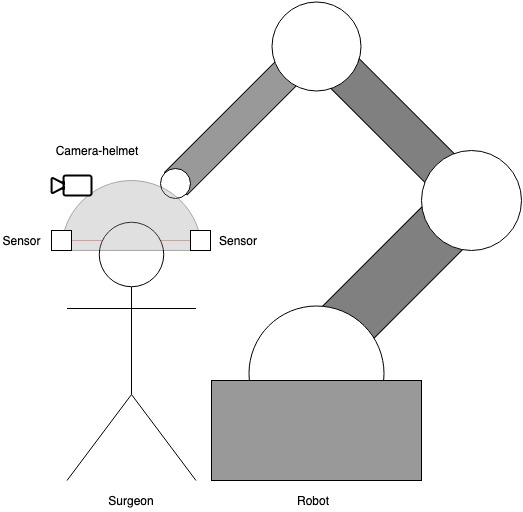
\includegraphics[width=5.5cm]{demo_mockup.jpg}
    \caption{An diagram of the sensor-helmet system.}
    \label{fig:demo_model}
\end{figure}
RobotStudio has a few of the components needed to build such a simulation. The robot arm, the virtual robot controller, and the virtual distance sensor are available. There is also a communication protocol available for ABB robot controllers called 'Externally Guided Motion' (EGM). The virtual controllers have the option to use EGM. The missing components for a simulation of the sensor-helmet are: retrieval of the sensor data, interpretation of the data into robot movement, and communication with the virtual controller via EGM.\par

From a practical standpoint, this project focused on simulating a part of the sensor-helmet system described above, i.e., the project attempted to solve the problem of missing simulation components for the sensor-helmet system by exploratory research of EGM and its technology dependencies (see section \ref{sec:Tech_Back}) and exploratory development of the required simulation components (see section \ref{sec:Dev}). From the standpoint of the project goals, this project generalized the work on the sensor-helmet problem for a wider range of applications and documented the results to act as a guide. The results of this project can be found in section \ref{sec:Result:LthRobotStudio} and a demonstration of the sensor-helmet simulation can be found in section \ref{sec:Result:Demo}. \par


\section{Justification of Work}
\label{sec:Intro:Justification}
As the use of sensor-controlled robotics grows, the need to be able to simulate these systems also grows. From the perspective of the author, this project represents the chance to learn about the process of programming robots as well as to explore a typical industry tool for robot programming in depth. From the perspective of the Robotics Laboratory, it is important to have a simulation environment that is usable for students and researchers. A functional framework for simulating sensor-control in RobotStudio has applications for the projects like the sensor-helmet research and similar projects.

\section{Limitations and Scope}
\label{sec:Intro:Limits_Scope}
This project is exploratory. At the time of writing, no research was found that was conducted on the topic of connecting virtual sensors to virtual robot controllers in a RobotStudio simulation. There were several areas that could have been explored more deeply but were not due to time constraints. One area that could have been explored more deeply was RobotStudio software development kit (SDK) \cite{ABB:RS_SDK}. Researching EGM and RAPID (the programming language for ABB robots) was prioritized over researching the RobotStudio SDK because the former concepts are applicable to both virtual robots in RobotStudio and real robots. As a consequence, the project goal to 'prototype a library of virtual sensors' was not pursued as fully as was proposed at the beginning of the project. Only one prototype virtual sensor was produced because much of the knowledge required to implement a virtual version of a real sensor falls in the RobotStudio SDK domain. That is all to say, this project on the 'simulation of sensor-controlled robotics' tended to focus on the 'controlled robotics' aspect rather than the 'simulation of sensor' aspect. 



%                                         |
%                                         |
%                                         |
%                                         |
%   _______                   ________    |
%  |ooooooo|      ____       | __  __ |   |
%  |[]+++[]|     [____]      |/  \/  \|   |
%  |+ ___ +|     ]()()[      |\__/\__/|   |
%  |:|   |:|   ___\__/___    |[][][][]|   |
%  |:|___|:|  |__|    |__|   |++++++++|   |
%  |[]===[]|   |_|_/\_|_|    | ______ |   |
%_ ||||||||| _ | | __ | | __ ||______|| __|
%  |_______|   |_|[::]|_|    |________|   \
%              \_|_||_|_/               jro\
%                |_||_|                     \
%               _|_||_|_                     \
%      ____    |___||___|                     \
%     /  __\          ____                     \
%     \( oo          (___ \                     \
%     _\_o/           oo~)/
%    / \|/ \         _\-_/_
%   / / __\ \___    / \|/  \
%   \ \|   |__/_)  / / .- \ \
%    \/_)  |       \ \ .  /_/
%     ||___|        \/___(_/
%     | | |          | |  |
%     | | |          | |  |
%     |_|_|          |_|__|
%     [__)_)        (_(___]
%
%   https://www.asciiart.eu/electronics/robots
%*********************************************************************
% TECHNICAL BACKGROUND
%*********************************************************************
\chapter{Technical Background}
\label{sec:Tech_Back}

\section{Overview}
\label{sec:Tech_Back:Overview}
To understand the framework that was developed over the course of this project, some terms and technologies will need definition and explanation.



\section{Robots and Robot Systems}
\label{sec:Tech_Back:Rob_Syst}
According to oxforddictionaries.com, a robot is "a machine capable of carrying out a complex series of actions automatically, especially one programmable by a computer" \cite{Def:Robot}. For the purposes of this paper, the term 'robot' will be further narrowed to mean a self-contained construct of mechanical devices, motors, electronics, and computer components sold by ABB as a 'robot'. That is to say, the term robot will refer to both the mechanical mechanisms and the robot controller. For examples, see \cite{ABB:Products}. \par
The term 'robot system' will be used to describe the complete ecosystem that a robot performs its tasks in. That system could include any number of: tools, objects, computers (external to the robot controller), sensors, and other mechanisms that are involved in the robot's task. 

\section{RobotWare}
\label{sec:Tech_Back:RobotWare}
The software that runs on ABB robot controllers is called RobotWare. It is important to distinguish between the RobotWare-OS, RobotWare options, and RobotWare add-ins \cite[Sec. 1]{ABB:controller_software}. RobotWare-OS is the operating system that runs on the robot controller. RobotWare options and add-ins are both software that run on top of the OS to add extra functionality to a robot. The difference is that ABB officially produces RobotWare options while add-ins are user made. 

\section{Line Sensors}
\label{sec:Tech_Back:Line_Sensors}
For the purposes of this paper, sensors are devices that measure some physical property. A line sensor measures the distance from itself to another object. 

\section{RAPID}
\label{sec:Tech_Back:Rapid}
RAPID is the programming language of ABB robots. RAPID code is stored and run on the robot controller. There are three main entities in the language: \textit{instructions}, \textit{functions}, and \textit{data types} \cite{ABB:rapid_instructions}. For the purposes of understanding this paper, it can be generally understood that: data types are defined configurations of values, functions perform operations on data types, and instructions are made up of a set of data types that the  controller uses to perform an action. 

\section{Robot Movement}
\label{sec:Tech_Back:Rob_Move}

\subsection{The convention used in this project}
\label{sec:Tech_Back:Rob_Move:conventions}
There are two main conventions used to describe the location of a robot. The first is to describe the angle of each joint of the robot . The second convention is to describe the \textit{position} and the \textit{orientation} of the robot. While both conventions are supported in the RobotWare-OS, the work done in the project used the position and orientation convention exclusively. This section is intended to be a 'crash course' in how the convention is used in the RobotWare-OS. 

\subsection{Default frames for position and orientation in RobotWare}
\label{sec:Tech_Back:Rob_Move:frames}
When talking about a robot's position, the convention is to use a single point on the robot or a tool that is attached to the robot (usually the point at which work is being done). In RobotWare, this point is called the tool center point (TCP). The TCP could be the tip of a tool attached to the end of the robot or (in the absence of a tool) it could be the anchor point for tools on the robot. However, the coordinates of the TCP alone are not enough to describe robot movement (or static positioning). If the TCP is positioned at the coordinates (5,5,5), in which direction is the tool pointed? With only the position of the TCP, it is impossible to discern if the tool is pointing from the floor 'upward' to the point (5,5,5) or if the tool is pointing 'downward' from the ceiling. To solve this problem, an orientation is used to describe the specific rotation of the tool around the TCP. However, this raises the issue of how to describe orientation.\\
The RobotWare-OS starts addressing the issue by defining local coordinate systems for each object it works with in reference to a global coordinate system. These coordinate systems are called frames. There are many defined frames in both the virtual controller in RobotStudio and the physical controllers \cite[Sec. 1.2.6]{ABB:robotstudio}, but for the purposes of understanding this project, only the frames of the TCP and the work object (Wobj) will be discussed.\\
The Wobj (which is defined in relation to a world frame or a robot base frame) is the default frame of reference for most robot controller activities. The user can define a Wobj but the default is called wobj0 which has its coordinate system origin defined at the base of the robot. The TCP is used as the origin of the Tool frame. A Tool frame is always defined such that the z-axis follows the direction of work for the tool, where the positive z goes from the TCP away from the tool and the negative z goes from the TCP into the body of the tool. In the case of a pen tool, the TCP would be the writing tip of the pen and the Tool frame z-axis would go through the body of the pen in the negative direction and towards the paper in the positive direction (see figure \ref{fig:TCP_frame}). The default Tool frame is called tool0 and has its TCP defined as the anchor point for tools at the end of the robot arm. The robot diagram in figure \ref{fig:wobj0_tool0} shows an example of the positioning of the wobj0 and tool0 frames. The notation of labeling the Wobj frame axes without primes (i.e. $x$) and the Tool frame axes with primes (i.e. $x^\prime$) will be continued in this section. 


\begin{figure}[H]
\centering
\begin{minipage}{.49\textwidth}
  \centering
  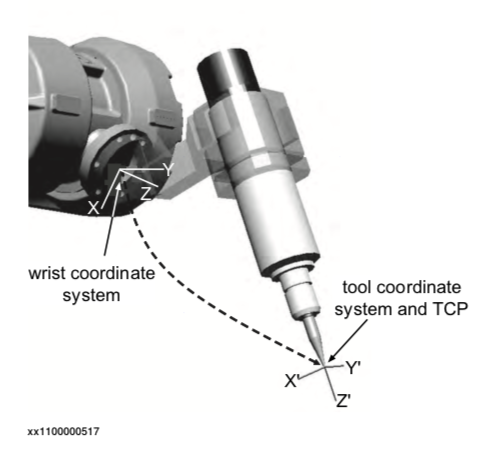
\includegraphics[width=5cm,height=5cm]{TCP_frame_3_88.png}
  \caption{Tool frame with z-axis out from TCP \cite[Sec. 3.88]{ABB:rapid_instructions}.}
  \label{fig:TCP_frame}
\end{minipage}%
\hspace{0.10cm}
\begin{minipage}{.49\textwidth}
  \centering
    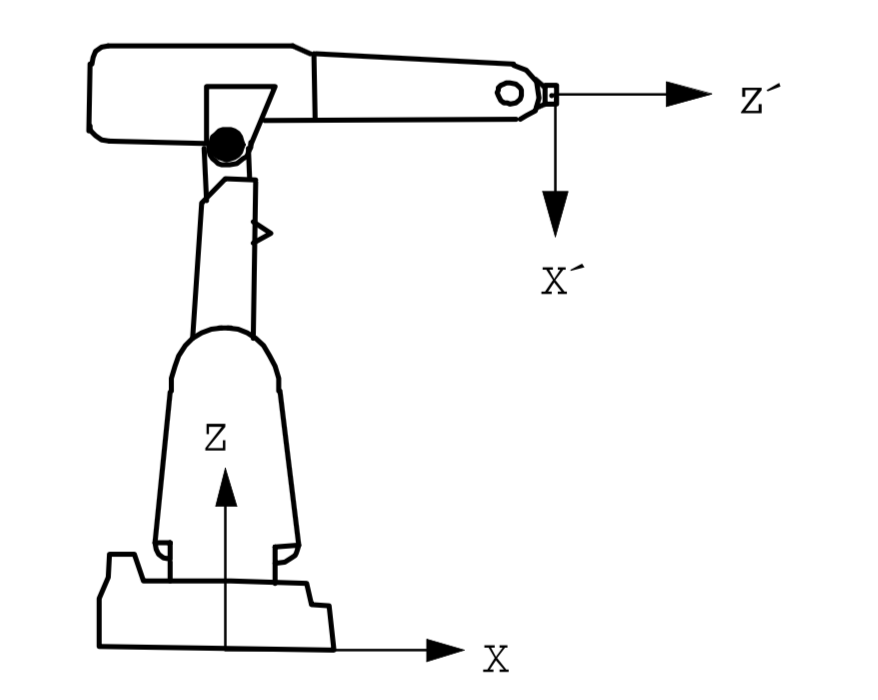
\includegraphics[width=5cm,height= 5cm]{wobj0_tool0.png}
    \caption{Wobj frame (wobj0) and Tool frame (tool0) \cite[Sec. 3.53]{ABB:rapid_instructions}.}
    \label{fig:wobj0_tool0}
\end{minipage}
\end{figure}


\subsection{A working definition of position and orientation.}
\label{sec:Tech_Back:Rob_Move:pos_orient}
This section will attempt to outline a useful working model of position and orientation. The following definitions are not as mathematically rigorous as they could be. Because readers of this paper are likely to fall into two categories (i.e. experienced with robotics or very new to robotics) the goal is to present enough information to understand the project. Any reader that has experience with Euler angels or quaternions to describe spatial orientations or rotations can skip to section \ref{sec:Tech_Back:Rob_Move:target_path} for how these concepts are applied in RAPID. It should also be noted that these definitions focus only on the Tool frame in relation to the Wobj frame, but the concepts extend to all other frames and coordinate systems in RobotWare.\par

\newpage
A frame is the unit vectors of a coordinate system. The two frames needed to define the position of the robot are the Wobj frame ($x$, $y$, $z$) and the Tool frame ($x^\prime$, $y^\prime$, $z^\prime$). The origin of the Tool coordinate system is the TCP. The position ($p$) of the robot is the coordinates of the TCP in the coordinate system given by the Wobj frame (see figure \ref{fig:rob_position}). That is to say: $p = (x_{t}, y_{t}, z_{t})$ regardless of the orientation of the Tool frame.

\begin{figure}[H]
\centering
\tdplotsetmaincoords{70}{110}
\begin{tikzpicture}[tdplot_main_coords]
    
    
    \draw[BrickRed,thick,->] (0,0,0) -- (3,0,0) node[anchor=north east]{$x$};
    \draw[OliveGreen,thick,->] (0,0,0) -- (0,4,0) node[anchor=north west]{$y$};
    \draw[Blue,thick,->] (0,0,0) -- (0,0,3) node[anchor=south]{$z$};
    \node[anchor=south east] at (0,0,0){\footnotesize{Wobj frame}};
    \tdplotsetrotatedcoords{30}{30}{0}
    \coordinate (O) at (0,0,0);
    \coordinate (S) at (1.0,3.5,1.25);
    
    \tdplotsetcoord{P}{3.85}{74.05}{71.05}
    
    \draw[dashed] (Px) -- (Pxy);
    \draw[dashed] (Py) -- (Pxy);
    \draw[dashed] (Px) -- (Pxz);
    \draw[dashed] (Pz) -- (Pxz);
    \draw[dashed] (Py) -- (Pyz);
    \draw[dashed] (Pz) -- (Pyz);
    \draw[dashed] (Pxy) -- (P);
    \draw[dashed] (Pxz) -- (P);
    \draw[dashed] (Pyz) -- (P);
    \node[anchor=east] at (Px){\footnotesize{$x_{t}$}};
    \node[anchor=south west] at (Py){\footnotesize{$y_{t}$}};
    \node[anchor=east] at (Pz){\footnotesize{$z_{t}$}};
    
    \tdplotsetrotatedcoordsorigin{(P)}
    \draw[thick,color=RubineRed,tdplot_rotated_coords,->] (0,0,0) --
        (2,0,0) node[anchor=west]{$x^\prime$};
    \draw[thick,color=Green,tdplot_rotated_coords,->] (0,0,0) --
        (0,2,0) node[anchor=south]{$y^\prime$};
    \draw[thick,color=Cerulean,tdplot_rotated_coords,->] (0,0,0) --
        (0,0,2) node[anchor=south west]{$z^\prime$};
    \node[anchor=north east, tdplot_rotated_coords] at (0,0,0){\footnotesize{Tool frame}};
\end{tikzpicture}
\caption{The position of the TCP (origin of the Tool frame) in reference to the Wobj frame.}
\label{fig:rob_position}
\end{figure}

The orientation of the robot is defined by the Tool frame's rotation in relation to the Wobj frame. In figure \ref{fig:rob_orientation}, there is a Wobj frame ($x$, $y$, $z$) with a Tool frame ($x^\prime$, $y^\prime$, $z^\prime$) overlaid such that the frames share the same origin. In the Wobj coordinate system, the $x$, $y$, and $z$ components of the Tool frame's x-axis are marked as $x_{x^\prime}$, $y_{x^\prime}$, and $z_{x^\prime}$ respectively. Put another way, with the Wobj frame as reference, the Tool frame's x-axis vector is: $x^\prime = (x_{x^\prime}, y_{x^\prime}, z_{x^\prime})$. In the same way, the y and z-axes of the Tool frame can be defined in terms of the Wobj frame as: $y^\prime = (x_{y^\prime}, y_{y^\prime}, z_{y^\prime})$ and $z^\prime = (x_{z^\prime}, y_{z^\prime}, z_{z^\prime})$. Using these vectors as columns, a rotation matrix for the Tool frame can be defined as: 

$$
\begin{bmatrix}
x_{x^\prime} & x_{y^\prime} & x_{z^\prime}\\
y_{x^\prime} & y_{y^\prime} & y_{z^\prime}\\
z_{x^\prime} & z_{y^\prime} & z_{z^\prime}
\end{bmatrix}
$$


Using this model, a quaternion orientation ($q_1$, $q_2$, $q_3$, $q_4$) is defined in \cite[Sec. 3.53]{ABB:rapid_instructions} as: 

%$$q_1 = \frac{\sqrt{x_{x^\prime} + y_{y^\prime} + z_{z^\prime} + 1}}{2}$$
%$$q_2 = \pm \frac{\sqrt{x_{x^\prime} - y_{y^\prime} - z_{z^\prime} + 1}}{2}$$
%$$q_3 = \pm \frac{\sqrt{y_{y^\prime} - x_{x^\prime} - z_{z^\prime} + 1}}{2}$$
%$$q_4 = \pm \frac{\sqrt{z_{z^\prime} - x_{x^\prime} - y_{y^\prime} + 1}}{2}$$
$$q_1 = \frac{\sqrt{x_{x^\prime} + y_{y^\prime} + z_{z^\prime} + 1}}{2} \; \; \; \; q_2 = \pm \frac{\sqrt{x_{x^\prime} - y_{y^\prime} - z_{z^\prime} + 1}}{2}$$
$$q_3 = \pm \frac{\sqrt{y_{y^\prime} - x_{x^\prime} - z_{z^\prime} + 1}}{2} \; \; \; \; q_4 = \pm \frac{\sqrt{z_{z^\prime} - x_{x^\prime} - y_{y^\prime} + 1}}{2}$$
where the signs of $q_2$, $q_3$, and $q_4$ are the same as ($z_{y^\prime} - y_{z^\prime}$), ($x_{z^\prime} - z_{x^\prime}$), and ($y_{x^\prime} - x_{y^\prime}$) respectively. 

\begin{figure}[H]
\centering
\tdplotsetmaincoords{70}{110}
\begin{tikzpicture}[tdplot_main_coords]
    
    
    \draw[BrickRed,thick,->] (0,0,0) -- (4,0,0) node[anchor=north east]{$x$};
    \draw[OliveGreen,thick,->] (0,0,0) -- (0,4,0) node[anchor=north west]{$y$};
    \draw[Blue,thick,->] (0,0,0) -- (0,0,4) node[anchor=south]{$z$};
    \tdplotsetrotatedcoords{45}{-45}{0}
    \coordinate (O) at (0,0,0);
    \coordinate (S) at (0,0,0);
    
    \tdplotsetcoord{P}{4}{45}{45}
    
    \draw[dashed] (Px) -- (Pxy);
    \draw[dashed] (Py) -- (Pxy);
    \draw[dashed] (Px) -- (Pxz);
    \draw[dashed] (Pz) -- (Pxz);
    \draw[dashed] (Py) -- (Pyz);
    \draw[dashed] (Pz) -- (Pyz);
    \draw[dashed] (Pxy) -- (P);
    \draw[dashed] (Pxz) -- (P);
    \draw[dashed] (Pyz) -- (P);
    \node[anchor=east] at (Px){\footnotesize{$x_{x^\prime}$}};
    \node[anchor=south west] at (Py){\footnotesize{$y_{x^\prime}$}};
    \node[anchor=east] at (Pz){\footnotesize{$z_{x^\prime}$}};
    
    \tdplotsetrotatedcoordsorigin{(S)}
    \draw[thick,color=	RubineRed,tdplot_rotated_coords,->] (0,0,0) --
        (4,0,0) node[anchor=west]{$x^\prime$};
    \draw[thick,color=Green,tdplot_rotated_coords,->] (0,0,0) --
        (0,4,0) node[anchor=south]{$y^\prime$};
    \draw[thick,color=Cerulean,tdplot_rotated_coords,->] (0,0,0) --
        (0,0,4) node[anchor=south west]{$z^\prime$};
\end{tikzpicture}
\caption{The projections ($x_{x^\prime}$, $y_{x^\prime}$, $z_{x^\prime}$) of the Tool frame x-axis ($x^\prime$) onto the Wobj frame axes ($x$, $y$, $z$).}
\label{fig:rob_orientation}
\end{figure}

While there are two possible ways for a user to describe the orientation of a Tool frame (i.e., Euler angels or quaternions), RobotWare really only accepts quaternions. There are functions in RAPID that will calculate the Euler angle for an axis from a quaternion orientation (see EulerZYX \cite[Sec. 2.64]{ABB:rapid_instructions}) or will calculate the quaternion from Euler angles (see OrientZYX \cite[Sec. 2.126]{ABB:rapid_instructions}), but the robot controller only accepts the quaternion orientation format for movement instructions. 

\subsection{Targets and paths}
\label{sec:Tech_Back:Rob_Move:target_path}
The way that RAPID represents a robot's position and orientation is with the \textit{pos} and \textit{orient} data types. A pos \cite[Sec. 3.56]{ABB:rapid_instructions} is an array of three numbers representing ($x$, $y$, $z$) coordinates in $mm$ (e.g. $[10.1, 20.2, 30.3]$). An orient data type \cite[Sec. 3.52]{ABB:rapid_instructions} is an array of four numbers representing the ($q_1$, $q_2$, $q_3$, $q_4$) values of a quaternion (e.g. $[1, 0, 0, 0]$). RAPID stored the position and orientation together as a \textit{target} in a data type called \textit{robtarget} \cite[Sec. 3.67]{ABB:rapid_instructions}. A robtarget (portmanteau of 'robot' and 'target') consists of four data types: a pos data type, an orient data type, a \textit{confdata} \cite[Sec. 3.17]{ABB:rapid_instructions} data type, and an \textit{extjoint}\cite[Sec. 3.34]{ABB:rapid_instructions} data type. A confdata data type describes joint configurations (e.g., the quadrant of the arm angle for a certain set of robot joints) and is dependant on the specific robot type being programmed. An extjoint data type describes the motion \textit{external joints} which are mechanical units that are external to the robot (i.e. part of the robot system but not part of the robot) that the robot controller has control of. This paper will assume that any confdata data types used are correct and that there are no external joints to control. An example of a robtarget can be found below in figure \ref{fig:RAPID_robtarget}. It is worth noting that the array of values given for the external joints are all '9E9' which indicate to the robot controller that there are no external joints to control. 

\lstset{language=RAPID}
\begin{figure}[H]
\centering
\begin{lstlisting}
! An example robtarget
CONST robtarget target_1 := [ 
    [600, 500, 400],                ! position data
    [1, 0, 0, 0],                   ! orientation data
    [1, 1, 0, 0],                   ! configuration data
    [9E9, 9E9, 9E9, 9E9, 9E9, 9E9]  ! external joints
];

\end{lstlisting}
\caption{Example of a robtarget in RAPID.}
\label{fig:RAPID_robtarget}
\end{figure}

Movement to a specific target is handled by move instructions in RAPID. There are several different move instructions available, but this explanation will focus on the relevant parts of the \textit{MoveL} \cite[Sec. 1.158]{ABB:rapid_instructions} instruction that relate to moving to a specific position and orientation. A code example of MoveL and its relevant arguments is provided for reference in figure \ref{fig:RAPID_movel}. MoveL is used to instruct the robot to move linearly to a specific target (i.e. move the TCP in a strait line to a given position and rotate the Tool frame to a specific orientation within a reference Wobj frame). The MoveL instruction has several required data types arguments as well as many optional arguments. The required argument names and their corresponding data are presented in the format of 'name':datatype as follows: 'ToPoint':robtarget, 'Speed':\textit{speeddata}, 'Zone':\textit{zonedata}, and 'Tool':\textit{tooldata}. The example in figure \ref{fig:RAPID_movel} also includes an optional argument: '\textbackslash WObj':\textit{wobjdata}. In the example code, all of the data types given to the MoveL instruction are predefined instances of each data type. 

\lstset{language=RAPID}
\begin{figure}[H]
\centering
\begin{lstlisting}
! Move linearly to the example target
MoveL  target_1 ,v100 ,fine ,tool0\WObj:=wobj0;
\end{lstlisting}
\caption{Example of MoveL instruction in RAPID.}
\label{fig:RAPID_movel}
\end{figure}

What follows is a brief explanation of the contents of each of the predefintions used in figure \ref{fig:RAPID_movel}, but for the full details of these data types refer to the documentation on speeddata \cite[Sec. 3.76]{ABB:rapid_instructions}, zonedata \cite[Sec. 3.103]{ABB:rapid_instructions}, tooldata \cite[Sec. 3.88]{ABB:rapid_instructions}, and wobjdata \cite[Sec. 3.100]{ABB:rapid_instructions}. The argument 'v100' is a speeddata that indicates that the TCP should be moved at a velocity ($v$) of $100 \; mm/s$, the Tool frame should be rotated at an angular velocity ($\omega$) of $500^\circ /s$ and that any linear or rotational external axes should be moved at $v = 5000 \; mm /s$ and $\omega = 1000^\circ /s$ respectively. The argument 'fine' is a zonedata that indicates that this movement instruction is considered complete only when the robot has reached the exact position and orientation given by the target and all the motors have come to a stop. The argument 'tool0' is a tooldata that has been discussed in section \ref{sec:Tech_Back:Rob_Move:frames} and represents the Tool frame in which the TCP is the physical anchor point on the robot for tools (see figure \ref{fig:wobj0_tool0}). The optional argument 'wobj0' tells the robot controller to use the wobj0 frame as reference for position and orientation of the tool (see figure \ref{fig:wobj0_tool0}). As it is optional to provide the move instruction with a Wobj frame for reference (the robot controller will use the active Wobj if a frame by default is not explicitly provided) the inclusion of this optional argument has to be prefaced with the command '\textbackslash WObj:='. That is all to say, the move instruction in figure \ref{fig:RAPID_movel} and the target in figure \ref{fig:RAPID_robtarget} can be read as: 
\begin{itemize}
    \item Move the tool anchor point in a strait line to the point (600 $mm$, 500$mm$, 400$mm$) from the robot base where $v = 100 \; mm /s$. 
    \item Rotate the tool anchor point to the same orientation as the base coordinate system where $\omega = 500^\circ / s$. 
    \item Stop all movement when the tool anchor point is exactly at the given point and rotation before continuing. 
\end{itemize}

The final component of robot motion in RAPID is the concept of a path. A path is simply a series of movement instructions. An example of a simple path can be found in figure \ref{fig:RAPID_target_path}. In this case, a second target (target\_2) is defined, then movement instructions to the targets are combined in a procedure called Ex\_Path. The path then goes from the current position of the robot via the point (600,500,400) in target\_1 to the point (400, 500, 600) in target\_2. 

\lstset{language=RAPID}
\begin{figure}[H]
\centering
\begin{lstlisting}
! a second target
CONST robtarget target_2 := [ 
    [400, 500, 600], 
    [1, 0, 0, 0], 
    [1, 1, 0, 0], 
    [9E9, 9E9, 9E9, 9E9, 9E9, 9E9] 
];
    
! A path
PROC Ex_Path()
    MoveL  target_1 ,v100 ,fine ,tool0\WObj:=wobj0;
    MoveL  target_2 ,v100 ,fine ,tool0\WObj:=wobj0;
ENDPROC
\end{lstlisting}
\caption{Example targets and a path in RAPID.}
\label{fig:RAPID_target_path}
\end{figure}

\subsection{Summary of robot motion in RAPID}
\label{sec:Tech_Back:Rob_Move:summary}
In summary, the motion of a robot is described in RAPID by a \textbf{path}. A path is composed of a series of \textbf{move instructions} where: a \textbf{target} to move a tool to, a \textbf{speed} at which to move, a \textbf{zone} around a target point where the robot's path is allowed to deviate from the straight line between target points, the \textbf{tool} that should be moved, and (optionally) a \textbf{frame of reference} for the motion are provided. A \textbf{target} contains a \textbf{position} and an \textbf{orientation}. \textbf{Positions} are given as ($x$, $y$, $z$) coordinates in $mm$. \textbf{Orientations} are given in ($q_1$, $q_2$, $q_3$, $q_4$) as quaternions. 


\section{RobotStudio}
\label{sec:Tech_Back:RobotStudio}
RobotStudio is the simulation environment that ABB supports for offline programming of their commercial robots. RobotStudio is capable of simulating robot systems. Simulated robots can be programmed from within RobotStudio via the RAPID editor. 

\section{Smart Components}
\label{sec:Tech_Back:Smart_Comp}
ABB supports several methods to modify RobotStudio beyond the basic functionality provided. One of these methods is the creation of smart components. Smart components are objects that can be simulated along side the robots and other components within RobotStudio. 

\section{Google Protocol Buffers}
\label{sec:Tech_Back:GPB}
Google Protocol Buffers is a "language-neutral, platform-neutral, extensible mechanism for serializing structured data" \cite{Google:Proto_Start}. To use Google Protocol Buffers, the data to be serialized is defined in a file with a .proto extension. The language guide for .proto files can be found at \cite{Google:Proto_v2_guide}. Once the protocol is defined in the .proto file, a compiler is used to create code in some supported language from the .proto file. E.g. compiling a protocol file called example.proto into python and java might result in the files example.py and example.java. With these files, a python program and a java program could use their respective files to serialize and deserialize example.proto messages \cite{Google:Proto_Api}.\par

ABB chose to define the EGM communication protocol with protocol buffers version 2. That is important because there was a dramatic change in version 3 that is not backwards compatible with version 2. Using protocol buffers to define the structure of the data in the UDP datagrams sent between the controller and the endpoint has one major advantage. The endpoint can be written in any language that can use protocol buffers to serialize and deserialize data. Although examples are given in the RobotWare documentation in C++ and C\#, a complete endpoint could be written in any of the languages mentioned in \cite{Google:Proto_Other}.

%  _________________________________________________________
% ||-------------------------------------------------------||
% ||.--.    .-._                        .----.             ||
% |||==|____| |H|___            .---.___|""""|_____.--.___ ||
% |||  |====| | |xxx|_          |+++|=-=|_  _|-=+=-|==|---|||
% |||==|    | | |   | \         |   |   |_\/_|Black|  | ^ |||
% |||  |    | | |   |\ \   .--. |   |=-=|_/\_|-=+=-|  | ^ |||
% |||  |    | | |   |_\ \_( oo )|   |   |    |Magus|  | ^ |||
% |||==|====| |H|xxx|  \ \ |''| |+++|=-=|""""|-=+=-|==|---|||
% ||`--^----'-^-^---'   `-' ""  '---^---^----^-----^--^---^||
% ||-------------------------------------------------------||
% ||-------------------------------------------------------||
% ||               ___                   .-.__.-----. .---.||
% ||              |===| .---.   __   .---| |XX|<(*)>|_|^^^|||
% ||         ,  /(|   |_|III|__|''|__|:x:|=|  |     |=| Q |||
% ||      _a'{ / (|===|+|   |++|  |==|   | |  |Illum| | R |||
% ||      '/\\/ _(|===|-|   |  |''|  |:x:|=|  |inati| | Y |||
% ||_____  -\{___(|   |-|   |  |  |  |   | |  |     | | Z |||
% ||       _(____)|===|+|[I]|DK|''|==|:x:|=|XX|<(*)>|=|^^^|||
% ||              `---^-^---^--^--'--^---^-^--^-----^-^---^||
% ||-------------------------------------------------------||
% ||_______________________________________________________||
%
%         https://www.asciiart.eu/books/books
%
%
%   _______________                        |*\_/*|________
%  |  ___________  |     .-.     .-.      ||_/-\_|______  |
%  | |           | |    .****. .****.     | |           | |
%  | |   0   0   | |    .*****.*****.     | |   0   0   | |
%  | |     -     | |     .*********.      | |     -     | |
%  | |   \___/   | |      .*******.       | |   \___/   | |
%  | |___     ___| |       .*****.        | |___________| |
%  |_____|\_/|_____|        .***.         |_______________|
%    _|__|/ \|_|_.............*.............._|________|_
%   / ********** \                          / ********** \
% /  ************  \                      /  ************  \
%--------------------                    --------------------
%
%        https://www.asciiart.eu/computers/computers
%*********************************************************************
% EXTERNALLY GUIDED MOTION 
%*********************************************************************
\chapter{Externally Guided Motion}
\label{sec:EGM}

\section{Overview}
\label{sec:EGM:Overview}
Externally Guided Motion (EGM) is a RobotWare option. That means that EGM is software that runs on top of the RobotWare-OS in both the robot controllers of a physical robot and virtual controllers in RobotStudio. EGM provides a way to control robot motion that is external to the RobotWare on the controller \cite[Sec. 9.3.1.1]{ABB:controller_software}. The core components involved in every usage of EGM are: the RAPID program, the motion control process, an EGM process, and an EGM endpoint. The motion control and EGM processes are concurrent threads of the controller software. An EGM endpoint is software external to the robot controller that communicates with an EGM process on the controller. By communicating with an EGM process, an endpoint obtains the current data about the state of the robot system and gives instructions to the controller \cite[Sec. 9.3.3]{ABB:controller_software}. An EGM process is started by the RAPID program and (once running) communicates directly with the motion control process of the robot controller. This direct communication means that movement instructions given through EGM bypass controller processes for path planning \cite[Sec. 9.3.1.3]{ABB:controller_software}. An EGM process can operate in several modes. These modes affect how movement instructions from an EGM endpoint are handled. In addition to the operational modes, there are many parameters that affect EGM. In the section discussing EGM, this paper will attempt to maintain the distinctions between the robot controller, the motion control process, and EGM processes because they are relevant to the parameters that affect EGM. Later sections tend not to make these distinctions as clear.  All usages of EGM share the basic structure outlined by the sequence diagram in figure \ref{fig:basic_egm}. 

\begin{figure}[H]
    \begin{center}
    \tikzset{every picture/.append style={transform shape, scale=1.05}}
    \begin{sequencediagram}
    %\renewcommand\unitfactor{0.5}
        \newthread{rapid}{RAPID Program}{}
        \newthread{mc}{Motion Control}{}
        \newinst{egm}{EGM Process}{}
        \newthread{end}{EGM Endpoint}{}
        \begin{messcall}{rapid}{start egm process}{egm}
            \begin{call}{egm}{get state}{mc}{state} 
            \end{call}
            \begin{call}{egm}{send state}{end}{movement} 
            \end{call}
            \begin{messcall}{egm}{movement}{mc}
            \end{messcall}
        \end{messcall}
        %\begin{call}{A}{EgmRobot}{B}{EgmSensor}
        %\end{call}
    \end{sequencediagram}
    \caption{Basic EGM sequence diagram.}
    \label{fig:basic_egm}
    \end{center}
\end{figure}

Regardless of the parameters or operational mode, an EGM process is started on the controller by a RAPID program. The EGM process then acts as a broker between the motion control process and an EGM endpoint. The rest of this section will document:
\begin{enumerate}
    \item How data is transferred between EGM processes and endpoints.
    \item The different operational modes of EGM processes.
    \item A general description of EGM endpoints.
    \item How EGM is handled in RAPID programs.
    \item The available parameters of EGM processes.
    \item The specific information sent between EGM processes and endpoints.
    \item Examples of RAPID programs and EGM endpoints.
\end{enumerate}

\section{EGM Transmission Protocols}
\label{sec:EGM:Trans_Protos}
Data transmission between EGM processes and EGM endpoints follow the user datagram protocol (UDP). The connection is established first by the robot controller with RAPID instructions (see section \ref{sec:EGM:Rapid_Programs}). The EGM endpoint acts as an UDP server for EGM messages from an EGM process. An EGM process must be able to correctly address EGM messages. In turn, an EGM endpoint must be able to receive EGM messages, extract meaningful information from the message, and send meaningful EGM messages back to the EGM process. Addressing for EGM processes is defined in the transmission protocol used when starting the EGM process (see section \ref{sec:EGM:Process_Management}). The structure of data sent between processes and endpoints (EGM messages) is defined by a Google Protocol Buffer file called egm.proto (see section \ref{sec:EGM:Message_Protos:message_v_protocol}). How these messages are handled by an EGM endpoint are addressed in section \ref{sec:EGM:Message_Protos:message_handling}. 


\section{EGM Process Modes}
\label{sec:EGM:Modes}
EGM processes can be used in three modes: position stream, position guidance, and path correction \cite[Sec. 9.3.1.1]{ABB:controller_software}. In every mode, the EGM process will send the the state data to an EGM endpoint. Movement instructions are sent by the endpoint to the EGM process. What the process does with the movement instructions is dependant on the mode as well as the process parameters (see section \ref{sec:EGM:Process_Management}). The format of the messages that are sent between the EGM process and the endpoint differ for each operational mode (see section \ref{sec:EGM:Message_Protos}). 

\subsection{Position stream}
\label{sec:EGM:Modes:stream}
The position stream mode of EGM is the least complicated mode. An EGM process running in position stream mode is intended to communicate the position of the robot (as well as other state information) to an EGM endpoint. The EGM endpoint is required to send responses to the controller to confirm that the UDP connection is functioning as it should, but these response messages do not affect the motion of the robot (i.e. the messages from the endpoint are ignored). More information on the position stream mode can be found in \cite[Sec. 9.3.1.2]{ABB:controller_software}.

\subsection{Position guidance}
\label{sec:EGM:Modes:guidance}
In position guidance mode, when an EGM process establishes a connection with an EGM endpoint, the execution of the RAPID program is stopped while movement instructions from the endpoint are executed \cite[Sec. 9.3.1.3]{ABB:controller_software}. During position guidance the controller streams the state data to an EGM endpoint and the endpoint responds by sending movement instructions to back to the EGM process. These movement instructions are passed to the motion control process and buffered. The instructions in the buffer are handled in first-in, first-out (FIFO) order. Full completion of a movement is not required to begin handling the next movement. I.e. if the motion control process retrieves an instruction to move to a target (e.g. $t_1$) from the buffer, it will begin to execute this instruction. It will also continue to regularly check the buffer for new instructions while executing the movement to $t_1$. If a new target (e.g. $t_2$) is retrieved from the buffer before the movement to $t_1$ is complete, movement to $t_2$ will begin immediately without reaching $t_1$. 

\subsection{Path correction}
\label{sec:EGM:Modes:corr}
In path correction mode, a path is defined with special movement instructions in the RAPID program and state data is streamed to the EGM endpoint while the movement instructions are being executed (see section \ref{sec:EGM:Rapid_Programs:corr}). While the aforementioned movement instructions are being executed, the EGM endpoint sends corrections to the EGM process. The controller uses these corrections to adjust the TCP's actual trajectory to be offset from (but nearly parallel to) the trajectory defined by the path \cite[Sec. 9.3.1.4]{ABB:controller_software}. To match the path trajectory, the controller will define a \textit{path correction frame} and will correct the position of the TCP within that frame according to corrections sent by the EGM endpoint (see figure \ref{fig:corr_frame}). The correction frame ($x^{\prime\prime}$, $y^{\prime\prime}$, $z^{\prime\prime}$) is defined in relation to the path and the orientation of the Tool frame ($x^{\prime}$, $y^{\prime}$, $z^{\prime}$). The direction of movement in the correction frame is given by $x^{\prime\prime}$. The $x^{\prime\prime}$-vector is always oriented as the tangent to the path in the direction of motion. The corrected position of the TCP is then given it terms of the orthogonal vectors ($y^{\prime\prime}$ and $z^{\prime\prime}$) to $x^{\prime\prime}$. The correction frame for the TCP at a position on the path is then given by the cross products: $y^{\prime\prime} = x^{\prime\prime} \times z^{\prime}$ and $z^{\prime\prime} = x^{\prime\prime} \times y^{\prime\prime}$. Corrections from an EGM endpoint are given as $y$ and $z$ values which the EGM process interprets as ($y^{\prime\prime}$, $z^{\prime\prime}$) coordinates in the correction frame. 

\begin{figure}[H]
\centering
\tdplotsetmaincoords{70}{110}
\pgfmathsetmacro{\ptheta}{60}
\pgfmathsetmacro{\pphi}{30}
\begin{tikzpicture}[tdplot_main_coords]
    
    \draw[BrickRed,thick,->] (0,0,0) -- (3,0,0) node[anchor=north east]{$x$};
    \draw[OliveGreen,thick,->] (0,0,0) -- (0,3,0) node[anchor=north west]{$y$};
    \draw[Blue,thick,->] (0,0,0) -- (0,0,3) node[anchor=south]{$z$};
    \tdplotsetrotatedcoords{0}{0}{70}
    \coordinate (O) at (0,0,0);
    \coordinate (S) at (1.0,3.5,1.25);
    \tdplotsetcoord{P}{3.464}{\ptheta}{\pphi}
    
    \tdplotsetrotatedcoordsorigin{(P)}
    
    \draw[tdplot_rotated_coords,->] (0,0,0) -- (0,0,-1) node[anchor=north]{$z^\prime$};
    \draw[dashed,tdplot_rotated_coords] (2.0,{0.5*cos(deg((2.0)*2.5))-0.5},0)
        \foreach \a in {2.0,1.99,...,-3.0}
        { -- ({\a}, {0.5*cos(deg(\a*2.5))-0.5}, {0})}node[anchor=east]{path};
    
    
    \draw[thick,color=RubineRed,tdplot_rotated_coords,->] (0,0,0) -- (1,0,0) node[anchor=west]{$x^{\prime\prime}$};
    \draw[thick,color=Green,tdplot_rotated_coords,->] (0,0,0) -- (0,1,0) node[anchor=west]{$y^{\prime\prime}$};
    \draw[thick,color=Cerulean,tdplot_rotated_coords,->] (0,0,0) -- (0,0,1) node[anchor=south]{$z^{\prime\prime}$};
    \draw[dashed,tdplot_rotated_coords] (0,0,0.5) -- (0,0.5,0.5);
    \draw[dashed,tdplot_rotated_coords] (0,0.5,0) -- (0,0.5,0.5) node[anchor=south west]{\footnotesize{TCP}};
   
\end{tikzpicture}
\caption{The position of the TCP within the path correction frame ($x^{\prime\prime}$, $y^{\prime\prime}$, $z^{\prime\prime}$) which is defined in relation to the Tool frame $z$-axis ($z^{\prime}$) and the path.}
\label{fig:corr_frame}
\end{figure}

It is important to note that, because the robot is trying to converge to a target given by the RAPID program, the path correction provided by the EGM endpoint needs to converge to zero by the time the robot is supposed to reach the destination target. If, for instance, the RAPID program defines a movement from the position (0, 0 ,0) to the position (10, 0, 0), the path with a correction of y=0 and z=0 would look like this: \{(0,0,0) (1,0,0), ..., (9,0,0), (10,0,0)\}. However, with a path correction of y=1 and z=0, the path would look this: \{(0,1,0) (1,1,0), ..., (9,1,0), (10,1,0)\}. This will cause the controller to throw an execution exception and the RAPID program will stop running. To prevent this, as the robot converges on the position (10, 0, 0), the offset needs to be y=0 and z=0 so that the robot actually reaches the target it is supposed to. 


\section{EGM Endpoints}
\label{sec:EGM:Endpoints}
An EGM endpoint is the destination of the robot system state data and the source for movement instructions bound for an EGM process. In order to interface with a robot controller via EGM, it is necessary for a programmer to implement an EGM endpoint. There are no restrictions on the functionality of the endpoint beyond the limitations of communicating with an EGM process. The limitations from the EGM process include: defined message structures (discussed in section \ref{sec:EGM:Message_Protos:proto_struct}), the three EGM modes, timing considerations, and requiring UDP as the transmission protocol. Beyond that, it is up to the programmer to implement the desired behavior of the EGM endpoint. There is a convention in ABB's documentation to refer to all EGM endpoints as 'sensors' \cite[Sec. 9.3.3]{ABB:controller_software}, but that convention will not be followed in this paper because it needs to maintain a distinction between the sensor mechanism and the software that handles UDP transmission of EGM protocol messages. ABB provides an example of an endpoint (egm-sensor.cs) in the RobotStudio files at \url{ABB Industrial IT\ Robotics IT\ RobotWare\ RobotWare_6.07.1011\ utility\ Template\ EGM\ }. In the folder, there are two versions of the example endpoint (one written in C++ and the other in C\#). The this project built upon the C\# example. 

\section{EGM RAPID Components}
\label{sec:EGM:Rapid_Components}
All EGM modes require some setup in the controller via RAPID commands. Examples of RAPID code for the different modes can be found in sections \ref{sec:EGM:Rapid_Programs:stream}, \ref{sec:EGM:Rapid_Programs:guidance}, and \ref{sec:EGM:Rapid_Programs:corr} for position stream, position guidance, and path correction respectively. The RAPID instructions used in this paper are briefly covered in figure \ref{fig:rapid_table} for reference: 

\begin{figure}[H]
\vspace{0.25cm}
    \centering
    \footnotesize{
    \begin{tabular}{| l | p{8cm} |}
    \hline
    \textbf{Component} &  \textbf{Description} \\ 
    \hline
    egmident & Reference to an EGM process \cite[Sec. 3.25]{ABB:rapid_instructions}  \\ \hline
    egmstate & Execution state of an EGM process \cite[Sec. 3.27]{ABB:rapid_instructions} \\ \hline
    egm\_minmax & Two values that limit linear or angular acceleration \cite[Sec. 3.26]{ABB:rapid_instructions} \\ \hline
    egmframetype & Describes the type of frame \cite[Sec. 3.24]{ABB:rapid_instructions}\\ \hline
    EGMGetState &   returns the egmstate of the process at a given egmident \cite[Sec. 2.63]{ABB:rapid_instructions}\\ \hline
    EGMGetId & Starts an EGM process and gets the egmident \cite[Sec. 1.68]{ABB:rapid_instructions}\\ \hline
    EGMReset & Resets an EGM process \cite[Sec. 1.71]{ABB:rapid_instructions} \\ \hline
    EGMSetupUC    & Assign a transmission protocol for an EGM process \cite[Sec. 1.78]{ABB:rapid_instructions} \\ \hline
    EGMStreamStart  & Start an EGM process streaming the robot position \cite[Sec. 1.80]{ABB:rapid_instructions} \\ \hline
    EGMStreamStop  &  Stop an EGM process streaming the robot position \cite[Sec. 1.81]{ABB:rapid_instructions} \\ \hline
    EGMActPose    & Setup position guidance mode for an EGM process \cite[Sec. 1.67]{ABB:rapid_instructions} \\ \hline
    EGMRunPose    & Start an EGM process running in position guidance mode  \cite[Sec. 1.73]{ABB:rapid_instructions} \\ \hline
    EGMActMove   & Setup path correction mode for an EGM process \cite[Sec. 1.66]{ABB:rapid_instructions} \\ \hline
    EGMMoveL    & A move instruction that is offset in path correction \cite[Sec. 1.70]{ABB:rapid_instructions} \\ \hline
    \end{tabular}
    }
    \caption{A table of relevant RAPID components.}
    \label{fig:rapid_table}
\end{figure}

\section{EGM Process Management}
\label{sec:EGM:Process_Management}
In order to send EGM messages to an endpoint via UDP, an EGM process needs to know the IP address and port number of the endpoint. The robot controller maintains a library of 'transmission protocols' that can be called for use in a RAPID program. A transmission protocol consists of a name, type, serial port, IP address, and IP port number. E.g. an EGM endpoint that is listening on port 8080 on the localhost, the transmission protocol in figure \ref{fig:process_comm} could be called by an EGM process to communicate with that endpoint by referring to 'endpoint\_address'. For details of how to access the library of transmission protocols through RobotStudio, see section \ref{sec:Dev:I1:RobotStudio_setup} or appendix \ref{app:Screenshots:Trans_protocols}. 
\begin{figure}[H]
    \centering
    \vspace{0.5cm}
    \begin{tabular}{|c|c|c|c|c|}
    \hline
\textbf{Name} & \textbf{Type} & \textbf{Serial Port} & \textbf{Remote Address} & \textbf{Remote Port Number}\\ \hline
endpoint\_address & UdpUc & N/A & localhost & 8080 \\ \hline
    \end{tabular}
    \caption{EGM process communication configuration example.}
    \label{fig:process_comm}
\end{figure}
\vspace{0.5cm}
There are also several parameters that need to be configured for each EGM process. The robot controller also maintains a library of predefined configurations sets of these required parameters. When the EGM RobotWare-option is activated (see \ref{sec:Dev:I1:RobotStudio_setup}) there is one predefined parameter configuration called 'default'. For details about how to access and add more parameter configurations to this library via RobotStudio, see section \ref{sec:Dev:I1:RobotStudio_setup} or appendix \ref{app:Screenshots:EGM_in_controller}. The values of the 'default' configuration can be found in figure \ref{fig:process_config}. 
\begin{figure}[H]
\vspace{0.5cm}
    \centering
    \begin{tabular}{| l | c |}
    \hline
        \textbf{Parameter} & \textbf{Value} \\ \hline
        Name        &   default \\
        Level       &   Filtering   \\
        Do Not Restart After Motors Off & No    \\
        Return to Programmed Position when Stopped & No \\
        Default Ramp Time & 2   \\
        Default Proportional Position Gain & 5  \\
        Default Low Pass Filter Bandwidth & 20  \\ \hline
    \end{tabular}
    \caption{The default EGM process configuration.}
    \label{fig:process_config}
\end{figure}
\vspace{0.5cm}
Before detailing the EGM process parameters, it is extremely important to provide a disclaimer concerning the validity of the information presented here. The information available regarding these parameters (taken from \cite[Sec. 9.3.2.5]{ABB:controller_software}, \cite[Sec. 9.3.4]{ABB:controller_software}, and \cite[Sec. 6.12]{ABB:system_parameters}) was not comprehensive enough to allow this paper to make many strong assertions of fact regarding their usage. Specifically, this paper will not assert that any claims made about the 'speed feed-forward' and 'speed reference' (as well as the affects that the process parameters have on them) are fact. It is clear that control signals for the servomotors are derived from messages sent by the EGM endpoint in some way and that these control signals are then passed through a control loop (see figure \ref{fig:lp_filter}). Unfortunately, information regarding either the mechanics of creating these control signals or the output of the control loop was not found. Consequently, several parts of the following explanation should be considered speculation. The decision to include this speculative information in the paper was made for two reasons. The first reason was that this speculative model of the control loop had predictive merit during the project (i.e. the result of changes to the parameters can be guess to some extent with this model). The second reason to include speculative information is to benefit any persons that might later use information in this project. If this speculative model of the control loop is inaccurate, the assumptions that led to the erroneous model should be documented. \par

Most of these parameters affect how movement instructions are translated into motor control signals in the robot. The exceptions are the parameters 'Do Not Restart After Motors Off' and 'Return to Programmed Position when Stopped' which define what the robot will do after the EGM process is stopped. The remaining parameters are pertinent to servomotor control signals and the control loop (see figure \ref{fig:lp_filter}). There are three levels an EGM process can operate on: raw, filtering, and path. When set to raw, the movement instructions are translated directly into motor control signals and passed directly to the servo controller (i.e. no gain or filtering applied to the control signals). Setting the level to filtering adds gain to the servo control signals and passes them through a low pass filter. The path level is required for EGM processes in path correction mode. The default ramp time is a value between $0 \; s$ and $10 \; s$ which sets the default time it takes for a movement to stop (e.g. if a servo needs to rotate $180^{\circ}$ to fulfill a movement instruction: a $10 \; s$ ramp time will mean the servo will be set to run at $18^{\circ}/s$ or $0.05 \; Hz$). Proportional position gain is applied to the servo control signals over the course of the movement. The gain starts at its default and is decreased by the sensor as the motor nears its target rotation. The default proportional position gain can be a value between $0.0$ and $20.0$. E.g. a proportional gain of $5.0$ would mean that an an input signal of $0.05 \; Hz$ would be sent to the servo controller as $0.25 \; Hz$. The default low pass filter bandwidth is a value between $0.0 \; Hz$ and $100.0 \; Hz$. E.g. a bandwidth of $20.0 \; Hz$ would filter out the servo signals used as examples for the previous parameters. It should be mentioned that this relationship between the motion instructions, the servo speed, and the servo signal frequencies constitutes the speculation previously mentioned. It is simply unclear from the documentation how desired servo speeds are mapped to servo signal frequencies. \par

\begin{figure}[H]
\vspace{0.5cm}
    \centering
    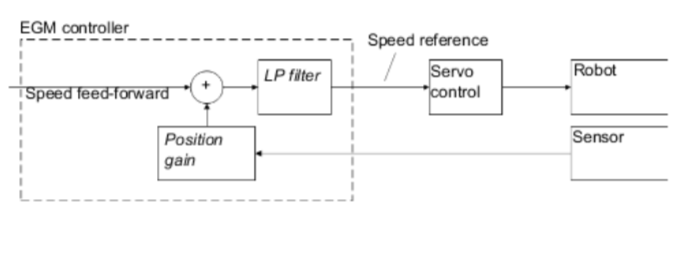
\includegraphics[width=12cm, height=5cm]{LP_filter_fig.png}
    \caption{Servo signal gain and filter during EGM \cite[Sec. 9.3.2.5]{ABB:controller_software}.}
    \label{fig:lp_filter}
\end{figure}


%!!!!!!!!!!!!!! EGM.PROTO !!!!!!!!!!!!!!!!!!!
\newpage
\section{EGM Message Protocols}
\label{sec:EGM:Message_Protos}

\subsection{Messages versus message protocols}
\label{sec:EGM:Message_Protos:message_v_protocol}
When discussing the way that information is communicated between an EGM process and an EGM endpoint, it is useful to make the following distinctions: 
\begin{itemize}
    \item A message protocol refers to the abstract structure of a message (i.e. defined in a Google Protocol Buffer .proto file)
    \item A message is a language specific instance of a message protocol (e.g. a C\# class that conforms to the structure of the message protocol)
    \item A serialization file contains language specific code for instantiating, serializing, and deserializing messages (serialization files are built for a specific language from the .proto file).
    \item A serialized message is a byte stream created by serializing a message from one language that can be de-serialized into the same message in other languages.
    \item Message data is the information stored in a message (can be primitive data types or submessages).
\end{itemize}
As stated in section \ref{sec:EGM:Trans_Protos}, communication between the robot controller and EGM endpoints follow UDP. I.e. serialized EGM messages are transmitted as the payload of UDP packets. When a UDP packet arrives at an endpoint, its payload is deserialized into an EGM message using the serialization file and the message data is read from the message. \par

A copy of the EGM message protocol (egm.proto) and its corresponding serialization files for C\# and Python (Egm.cs and egm\_pb2.py) can be found at \cite{Greg:Ref_Repo} in the 'Protocols' folder. 

\subsection{EGM message protocol structure}
\label{sec:EGM:Message_Protos:proto_struct}
The EGM message protocol (egm.proto) defines three main message types: EgmRobot, EgmSensor, and EgmSensorPathCorr. The definitions and usage of these messages are dependant on the EGM process mode. Processes send robot state data to endpoints in the form of EgmRobot messages. Endpoints in turn send movement instructions to the controller in the form of EgmSensor or EgmSensorPathCorr messages. Because Google protocol buffer messages are intended to standardize data transfer in object-oriented languages, the structure of message protocols is similar to an  object-oriented class hierarchy. Therefore, the EGM message protocol will be presented using a slight variation on a class diagram. The protocol diagram in figure \ref{fig:egm_proto} describes the messages defined in egm.proto. Message types are represented as classes would be. Message types are defined by the submessages they contain. In the protocol diagram, submessages are analogous to class attributes and are listed in 'name:type' format. A submessage can be either a base data type (e.g. int, bool, double) or another message type. When a submessage is a message type, the definition of the submessage type is connected to the message with an association arrow. The modifiers on the submessage fields in figure \ref{fig:egm_proto} (and other message protocol diagrams in the paper) do not describe the accessibility of the field as they would in standard UML. In this case, the modifiers describe the requirement level of a submessage. The requirement level modifiers used are $+$, $-$, and \& which denote optional, required, and repeated submessages respectively. In the case of a submessage of type 'enum', the enumerated names and values included in the message's bottom section (where class methods would be in a class diagram). The decision was made to keep figure \ref{fig:egm_proto} a large size in order to make it easier for a programmer to referrer to while working with EGM messages.
\begin{figure}[H]
    \centering
    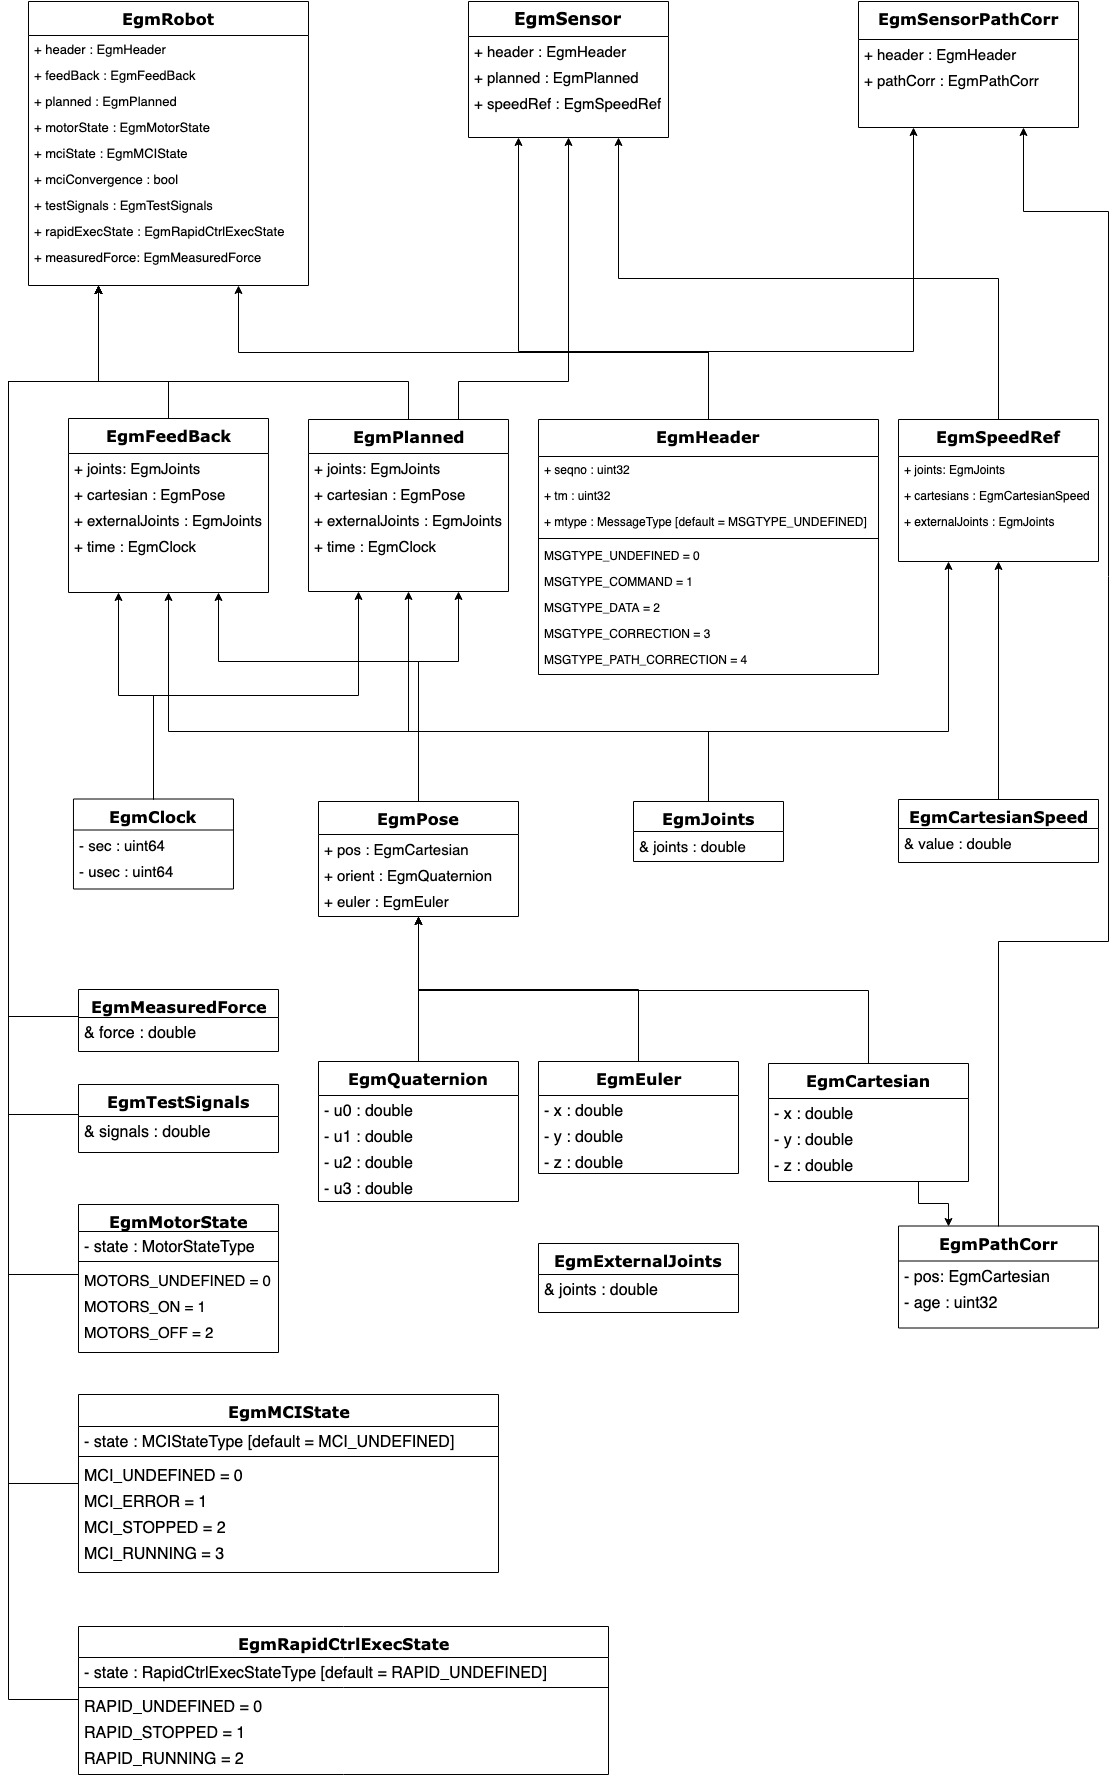
\includegraphics[width=12cm]{egm_proto_v2.jpg}
    \caption{The message structure of the EGM protocols.}
    \label{fig:egm_proto}
\end{figure}


\subsection{EgmRobot: robot state data protocol}
\label{sec:EGM:Message_Protos:EgmRobot}
When an EGM process sends state data to an EGM endpoint, an EgmRobot message is used (see figure \ref{fig:egm_proto} for the EgmRobot message protocol). To this point, the information sent to an endpoint has been broadly referred to as 'robot state data' or 'state data'. Before discussing how such messages can be used by an EGM endpoint (see section \ref{sec:EGM:Message_Protos:message_handling}), it would be useful to briefly summarize the 'state data' that is in an EgmRobot message. EgmRobot has nine sub messages. The submessages fall into three categories: header, robot system position data, and robot system state data. Broadly speaking, the position data should also be considered robot system state data. However, exclusively for the purposes of explaining the EgmRobot message protocol, it is useful to distinguish between 'position' and 'state' data. The header (header : EgmHeader) contains a sequence number (seqno : uint32), time stamp (tm : uint32) and message type (mtype : MessageType). The position data includes the current position of the robot system (feedBack : EgmFeedBack) and the next planned position (planned : EgmPlanned). The EgmFeedBack and EgmPlanned message protocols are identical and they contain information that corresponds to the information in the robtarget (section \ref{sec:Tech_Back:Rob_Move:target_path}) RAPID data type. The EgmPlanned message is discussed in more detail in relation to the EgmSensor protocol (see section \ref{sec:EGM:Message_Protos:EgmSensor}). It is, however, worth noting that an EgmPlanned message contains a target slightly ahead of the TCP when it is a part of an EgmRobot message. When used in a EgmSensor message, the EgmPlanned submessage contains movement instructions. The state data is described by the remaining six submessages. The motor state (motorState : EgmMotorState) can be: undefined, on, or off. The EGM state (mciState : EgmMCIState) can be: undefined, error, stopped, or running. The EGM state of the EgmRobot message corresponds to the EGM process states (figure \ref{fig:process_diagram}) in that a process transitioning from a connected to running state will correspond to the EgmMCIState transitioning from stopped to running. The convergence (mciConvergenceMet : bool) indicates if the current target has been reached by the robot or if motion towards the current target is ongoing. The test signals (testSignals : EgmTestSignals) are described in the comments of egm.proto as "[t]est signals". No further information on the use of the test signals was found. The RAPID execution state (rapidExecState : EgmRapidCtrlExecState) can be: undefined, stopped, or running. The measured force (measuredForce : EgmMeasuredForce) is described in the comments of egm.proto as an "[a]rray of 6 force values for a robot". It could be inferred that these values are meant to be forces on the robot joints, but that is speculation. No further information was found regarding the measured force and all values observed sent from the virtual controller were zero.

\subsection{EGM message handling in endpoints}
\label{sec:EGM:Message_Protos:message_handling}
In this context of EGM, message handling involves: reading and writing the data of EGM messages, serialization and deserialization of EGM messages, and transmission of the serialized EGM messages. In any EGM endpoint, the state data being sent from the EGM process in the robot controller (i.e. state data in an EgmRobot message) will have to be handled. Depending on the mode, either an EgmSensor or EgmSensorPathCorr message will also need to be handled. E.g. a simple task in a C\# endpoint would be to create an array of doubles to hold the current x, y, and z coordinates of the TCP (see figure \ref{fig:parse_egmrobot}). 

\lstset{language=[Sharp]C}
\begin{figure}[H]
    \centering
    \begin{lstlisting}
using System.Net;
using System.Net.Sockets;
using abb.egm;      
// Receive byte[] from any IP address on a port
UdpClient udpServer = new UdpClient(_portNbr);
IPEndPoint remoteEP = new IPEndPoint(IPAddress.Any, _portNbr);
byte[] data = udpServer.Receive(ref remoteEP);
// De-serialize the byte[] into an instance of EgmRobot
EgmRobot robot= EgmRobot.CreateBuilder().MergeFrom(data).Build();
// Extract state data from the EgmRobot message
double[] currentCoordinates = new double[] {
    robot.FeedBack.Cartesian.Pos.X,
    robot.FeedBack.Cartesian.Pos.Y,
    robot.FeedBack.Cartesian.Pos.Z};
\end{lstlisting}
    \caption{Example of accessing state data from an EgmRobot message.}
    \label{fig:parse_egmrobot}
\end{figure}

\lstset{language=[Sharp]C}
\begin{figure}[H]
    \centering
    \begin{lstlisting}
using abb.egm; 
// Instantiate a builder for an EgmSensor message
EgmSensor.Builder sensor = EgmSensor.CreateBuilder();
// Instantiate a builder for an EgmHeader message
EgmHeader.Builder hdr = new EgmHeader.Builder();
// Set the data for the EgmHeader
hdr.SetSeqno((uint)_seqNbr++)
 .SetTm((uint)DateTime.Now.Ticks)
 .SetMtype(EgmHeader.Types.MessageType.MSGTYPE_CORRECTION);
// Set EgmSensor.header <- EgmHeader message 
sensor.SetHeader(hdr);
// Builders for EgmPlanned, EgmPose, and EgmCartesian msg
EgmPlanned.Builder planned = new EgmPlanned.Builder();
EgmPose.Builder position = new EgmPose.Builder();
EgmCartesian.Builder cartesian=new EgmCartesian.Builder();
// Set some data to send. The coordinates are given in mm.
cartesian.SetX(1.111)
      .SetY(2.222)
      .SetZ(3.333);
position.SetPos(cartesian);
planned.SetCartesian(position);
sensor.SetPlanned(planned);
// Finally, serialize the the EgmSensor message.
EgmSensor serializedMessage = sensor.Build();
\end{lstlisting}
\caption{Example of building, serializing, and transmitting an EgmSensor message.}
\label{fig:build_egm_sensor}
\end{figure}
\vspace{0.5cm}
In this example endpoint, a serialized EgmRobot message is transmitted to the endpoint via the udpServer, an instance of EgmRobot message is created by deserializing the data from the udpServer, and the position data is read from the message. As previously mentioned, there are two types of response message that an EGM endpoint sends back to its EGM process. When using position stream and position guidance, the EGM process expects a response in the form of an EgmSensor message. Path correction requires a response in the form of an EgmSensorPathCorr message. An example of building and serializing an EgmSensor message can be found in figure \ref{fig:build_egm_sensor}. The process of building and serializing an EgmSensorPathCorr message is the same as for an EgmSensor.





\subsection{EgmSensor: movement instruction protocol}
\label{sec:EGM:Message_Protos:EgmSensor}
When programming an EGM endpoint (assuming that the connection with the EGM process is made and maintained) there is a finite set of values that can be sent to the robot controller. If the endpoint is communicating with an EGM process that is running in either position stream or position guidance mode, the message sent in an EgmSensor. The structure of EgmSensor messages can be found in figure \ref{fig:egm_sensor} below. \par 
\begin{figure}[H]
\vspace{0.30cm}
    \centering
    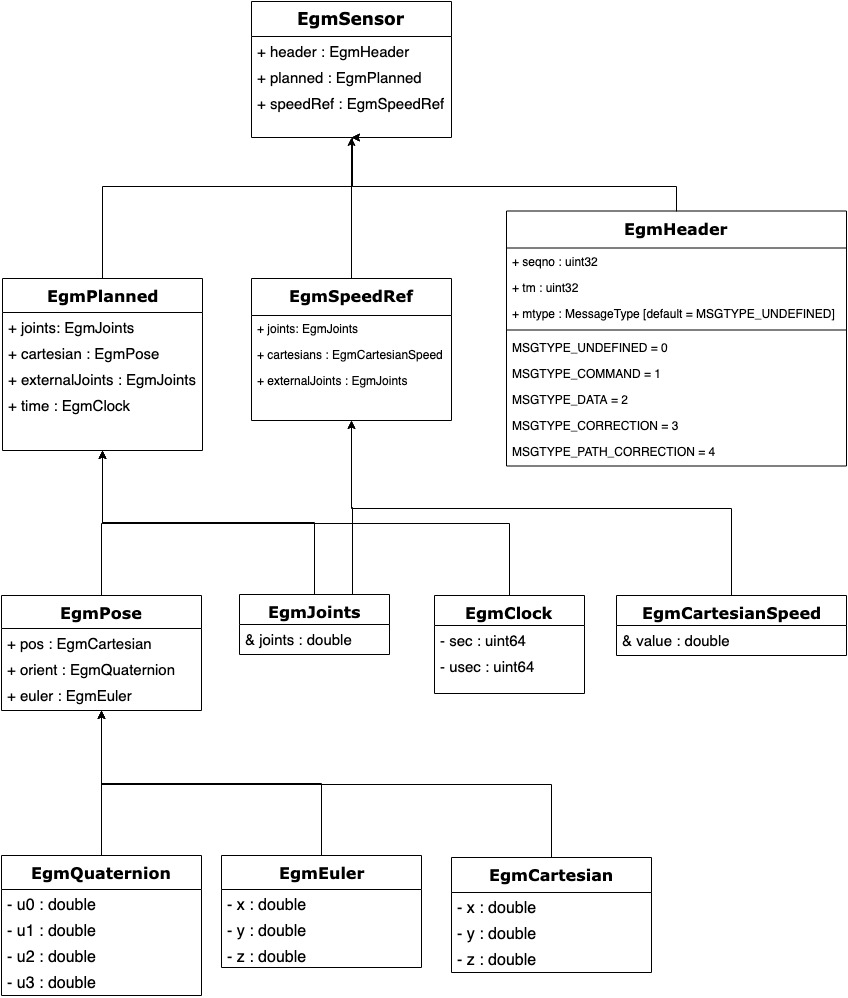
\includegraphics[width=10cm]{egm_sensor_proto_spelling.jpg}
    \caption{The structure of EgmSensor messages.}
    \label{fig:egm_sensor}
\end{figure}

The header (header : EgmHeader) has three submessages: the sequence number (seqno : uint32), the time stamp (tm : uint32), and the message type (mtype : MessageType). Of the message data in the header, the robot controller only uses the message type. The sequence number and time stamp can be useful for debugging purposes, but they are not used by the controller. When communicating with an EGM process in position stream or position guidance mode, the message type should be set to {\scriptsize{MSGTYPE\_CORRECTION}}. When using Path Correction mode, the message type in the header of the EgmSensorPathCorr message should be set to {\scriptsize{MSGTYPE\_PATH\_CORRECTION}}.\par
The message data for the movement instruction is contained in the planned submessage (planned : EgmPlanned). The movement instructions can be described by either using the joint values convention (joints  : EgmJoints) or using the position and orientation convention (cartesian : EgmPose). For information on robot motion conventions, see section \ref{sec:Tech_Back:Rob_Move}. EgmJoints are given in degrees as an array of 6 doubles. EgmPose contains submessages for position (pos : EgmCartesian) and orientation in either quaternions (orient : EgmQuarternion) or Euler angles (euler : EgmEuler). EgmCartesian messages contain x, y, and z submessages (x : double, y : double, z : double). The unit expected by the controller for the position values is  $mm$. If an EgmSensor message contains both quaternion and Euler angles, the virtual controller will prioritize the Euler angles. If no orientation is given, the controller will use the closest possible orientation to its current orientation. The planned submessage also includes fields for external joints (externalJoints : EgmJoints) and an absolute time (time : EgmClock). The external joint values are analogous to the extjoint data type in a robtarget in RAPID (section \ref{sec:Tech_Back:Rob_Move:target_path}). The time can be given in $s$ (sec : uint64) or $\mu s$ (usec : uint64) as an absolute number of $s$ or $\mu s$ since 1 Jan 1970. While such an absolute time could be useful in debugging, it is unclear if this field is utilized by the robot controller in any way. \par

The final submessage of an EgmSensor message is a speed reference (speedRef : EgmSpeedRef). An EgmSpeedRef message contains two EgmJoint submessages (joints : EgmJoint) and (externalJoints : EgmJoint) as well as an EgmCartesianSpeed submessage (cartesians : EgmCartesianSpeed). According to the code comments in egm.proto, an EgmSpeedRef message is "speed reference values for robot (joint or cartesian) and additional axis (array of 6 values)" and an EgmCartesianSpeed message is "Array of 6 speed reference values in mm/s or degrees/s". While it is unclear exactly how the speedRef submessage is intended to be used from this documentation, speedRef is probably in reference to the 'Speed reference' label in figure \ref{fig:lp_filter}. \par

\subsection{EgmSensorPathCorr: correction protocol}
\label{sec:EGM:Message_Protos:EgmSensorPathCorr}
EgmSensorPathCorr messages are used for EGM processes in path correction mode. The EgmSensorPathCorr message contains a header (header : EgmHeader) and corrections (pathCorr : EgmPathCorr). The header of an EgmSensorPathCorr should have the message type (mtype : MessageType) set to {\scriptsize{MSGTYPE\_PATH\_CORRECTION}}. The corrections are given as a position (pos : EgmCartesian). Only the y and z values of position are used by the robot controller (see section \ref{sec:EGM:Modes:corr} for more detail). There is also a submessage for age (age : uint32). It is unclear if the age is used by the controller, but according to the code comments in egm.proto age is the "sensor measurement age in ms". \par


\section{RAPID programs for EGM modes}
\label{sec:EGM:Rapid_Programs}
The following code examples are based on the RAPID code examples provided for Position Stream \cite[Sec. 9.3.6.1]{ABB:controller_software}, Position Guidance \cite[Sec. 9.3.6.2]{ABB:controller_software} and Path Correction  \cite[Sec. 9.3.6.3]{ABB:controller_software}. They have been altered to use the same naming conventions as consistently as possible in each example. Unless otherwise stated, these examples will all assume the following setup: an EGM endpoint listening at port 8080, a virtual controller named ROB\_1, the RobotWare-option for EGM enabled for ROB\_1, the transmission protocol presented in section \ref{sec:EGM:Process_Management} defined for ROB\_1, the 'default' EGM process configuration (see section \ref{sec:EGM:Process_Management})




%*******************************************************************
% POSITION STREAM --------------------------------------------------
%*******************************************************************
\subsection{RAPID for EGM position stream}
\label{sec:EGM:Rapid_Programs:stream}
Position streaming is used in situations where there is a need to "provide external equipment with the current and planned positions of mechanical units that are controlled by the robot controller." \cite[Sec. 9.3.1.1]{ABB:controller_software}. This means that the EGM endpoint will act as a receiver for the external equipment but movement instructions sent back to the EGM process will be ignored. An example RAPID program and a corresponding sequence diagram for EGM position streaming is provided in figure \ref{fig:rapid_pos_stream} and figure \ref{fig:sequence_pos_stream} respectively. \par

\lstset{language=RAPID}
\begin{figure}[H]
    \centering
    \begin{lstlisting}
CONST robtarget Home;
CONST robtarget Target_10;
CONST robtarget Target_20;
VAR egmident egmProc;
! Main process
PROC main()
    MoveL Home,v100,fine,tool0\WObj:=wobj0;
    ! Start the Stream procedure
    Stream;
ENDPROC
! The Path_10 procedure is just move instructions 
PROC Path_10()
    MoveJ Target_10,v100,fine,tool0\WObj:=wobj0;
    MoveJ Target_20,v100,fine,tool0\WObj:=wobj0;
ENDPROC
! The EGM position stream procedure
PROC Stream()
    EGMGetId egmProc;
    EGMSetupUC ROB_1, egmProc, "default", "endpoint_address"\Pose;
    EGMStreamStart egmProc\SampleRate:=16;
    Path_10;
    EGMStreamStop egmProc;
    EGMReset egmProc;
ENDPROC

\end{lstlisting}
\caption{Example RAPID program for EGM Position Stream.}
\label{fig:rapid_pos_stream}
\end{figure}


\begin{figure}[H]
\vspace{2cm}
    \begin{center}
    \tikzset{every picture/.append style={transform shape, scale=1.1}}
    \begin{sequencediagram}
        \newthread{rapid}{\scriptsize{ : RAPID Program}}{}
        \newinst{rob1}{\scriptsize{ROB\_1 : Motion Control}}{}
        \newinst{egm}{\scriptsize{egmProc : EGM Process}}{}
        \newthread{end}{\scriptsize{ : EGM Endpoint}}{}
\scriptsize{
        \begin{call}{rapid}{MoveL Home}{rob1}{return}
        \end{call}
        \begin{sdblock}{Stream()}{}
        \begin{messcall}{rapid}{EGMGetId egmProc}{egm}
            \begin{messcall}{rapid}{EGMSetupUC ROB\_1, "default", "endpoint\_address"}{egm}
            \end{messcall}
            \begin{messcall}{rapid}{EGMStreamStart egmProc}{egm}
                \begin{callself}{egm}{EGMStreamStart $\rightarrow$ loop start}{EGMStreamStop $\rightarrow$ loop stop} 
                    %\mess[1]{egm}{get state}{rob1}
                    %\mess[1]{rob1}{return state}{egm}
                    \setthreadbias{east}
                    \begin{call}{egm}{get state}{rob1}{return state}
                        \postlevel
                    \end{call}
                    \setthreadbias{center}
                    %\mess[1]{egm}{send state}{end}
                    %\mess[1]{end}{return message}{egm}
                    \begin{call}{egm}{EgmRobot}{end}{EgmSensor}
                    \end{call}
                    %\mess{rapid}{}{egm}
                \end{callself}
            \end{messcall}
            
            \prelevel\prelevel\prelevel\prelevel\prelevel\prelevel\prelevel
            
            \begin{callself}{rapid}{Path\_10()}{Finish Path\_10()} 
                %\mess[1]{rapid}{Move Instruction}{rob1}
                %\mess[1]{rob1}{return}{rapid}
                \begin{call}{rapid}{Move Instruction}{rob1}{return}
                    \postlevel
                \end{call}
            \end{callself}
            \begin{messcall}{rapid}{EGMStreamStop egmProc}{egm}
            \end{messcall}
            \prelevel
            \mess{rapid}{EGMReset egmProc}{egm}
        \end{messcall}
        \end{sdblock}
        %\mess{rapid}{}{egm}
}
        %\begin{call}{A}{EgmRobot}{B}{EgmSensor}
        %\end{call}
    \end{sequencediagram}
    \end{center}
    \caption{Sequence diagram for EGM position Stream.}
    \label{fig:sequence_pos_stream}
\end{figure}
\vspace{1.5cm}
It is worth noting that once EGMStreamStart egmProc\textbackslash SampleRate:=16 is called in the RAPID program, the EGM process starts a loop that gets and sends the robot state data every 16 $ms$. From start to return, a 'Move Instruction' that is called during Path\_10() can take seconds or minutes. That means that the state data will probably called many times while the robot is moving to any given target.
%*******************************************************************




%*******************************************************************
% POSITION GUIDANCE ------------------------------------------------
%*******************************************************************
\subsection{RAPID for EGM position guidance}
\label{sec:EGM:Rapid_Programs:guidance}
Setting up an EGM process to use for position guidance requires a few more steps. Because position guidance requires two way communication with an EGM endpoint, the robot controller will need to manage to the state of the EGM process. The \cite[Sec. 9.3.2.2]{ABB:controller_software} provides a state diagram for EGM processes that can be found in figure \ref{fig:process_diagram}. \par

\vspace{2cm}
\begin{figure}[H]
    \centering
    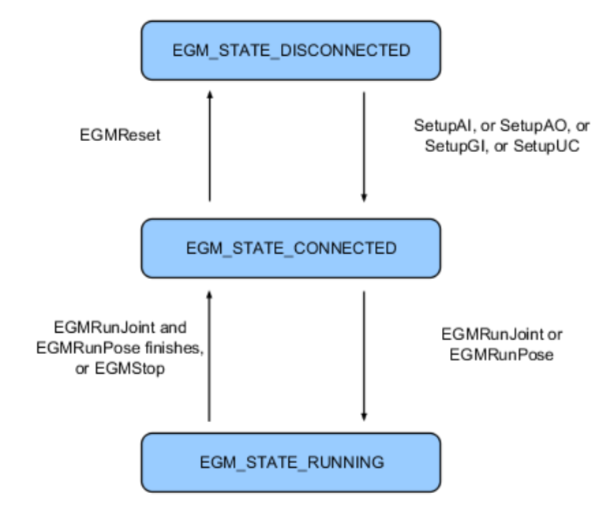
\includegraphics[width=9.5cm]{pic_process-state-diagram.png}
    \caption{EGM process state diagram.}
    \label{fig:process_diagram}
\end{figure}
State management is relevant for position guidance (and path correction) because it allows the RAPID program to confirm that the EGM process has established a connection with the EGM endpoint before it allows the EGM process to control the motion of the robot. This means, to check the UDP connection with an endpoint, the structure of the position guidance RAPID program should be:
\begin{enumerate}
    \item Execute a 'fine' movement to a start position
    \item Test the UDP connection by checking the EGM process state
    \item If the state is {\scriptsize{EGM\_STATE\_DISCONNECTED}} or {\scriptsize{EGM\_STATE\_CONNECTED}}: run position guidance.
\end{enumerate}
A RAPID program for position guidance with this structure can be found in figure \ref{fig:rapid_pos_guide}. The corresponding sequence diagram for the example program can be found in figure \ref{fig:sequence_pos_guide}.
\lstset{language=RAPID}
\begin{figure}[H]
\vspace{0.75cm}
\centering
\begin{lstlisting}
! Example assumes the definition of the Home.
CONST robtarget Home;
! Declare an EGM process called egmProc
VAR egmident egmProc;
VAR egmstate egmSt;
CONST egm_minmax minmax_lin:=[-1,1];
CONST egm_minmax minmax_rot:=[-2,2];
VAR pose corr_frame_offs:=[[0,0,0],[1,0,0,0]];

PROC main()
    MoveL Home,v100,fine,tool0\WObj:=wobj0;
    test_UDP;
ENDPROC
	
PROC test_UDP()
    EGMReset egmProc;
    EGMGetId egmProc;
    egmSt:=EGMGetState(egmProc);
    IF egmSt<=EGM_STATE_CONNECTED THEN
        EGMSetupUC ROB_1,egmProc,"default","endpoint_address"\pose;
    ENDIF
    runEGM;
    egmSt1:=EGMGetState(egmProc);
    IF egmSt=EGM_STATE_CONNECTED THEN
        EGMReset egmProc;
    ENDIF
ENDPROC
    
PROC runEGM()
    EGMActPose egmProc \Tool:=tool0 \WObj:=wobj0,
        corr_frame_offs,EGM_FRAME_WOBJ,
        corr_frame_offs,EGM_FRAME_WOBJ
        \x:=minmax_lin \y:=minmax_lin \z:=minmax_lin
        \rx:=minmax_rot \ry:=minmax_rot \rz:=minmax_rot
        \LpFilter:=2 \Samplerate:=4 \MaxSpeedDeviation:=2;
    EGMRunPose egmProc,EGM_STOP_HOLD \x \y \z
        \CondTime:=10 \RampInTime:=0.05 \RampOutTime:=0.05;
ENDPROC
    \end{lstlisting}
    \caption{Example RAPID program for EGM Position Stream.}
    \label{fig:rapid_pos_guide}
\end{figure}

This program can be broken down into four distinct stages: robot setup, connection setup, position guidance setup, and position guidance execution. The robot setup stage requires that the robot be moved into a starting position. It is extremely important that this bust be a fine movement because the robot controller needs to know its starting position with the greatest degree of accuracy possible. If the move instruction is not a fine movement, the controller will simply not execute any EGM instructions in the RAPID code. \par

Once the fine movement to a target is complete, the connection setup can begin. Although it should not happen in this example program, it is possible that a given EGM process could still be in a state of {\scriptsize{EGM\_STATE\_RUNNING}} in a more complicated program. It is recommended good practice to reset EGM processes (EGMReset) before using them. EGMGetId will instantiate an EGM process if one is not already attached to the egmident 'egmProc'. EGMGetState will return the state of the EGM process. The condition 'egmSt $<=$ {\scriptsize{EGM\_STATE\_CONNECTED}}' will be true if the state is {\scriptsize{EGM\_STATE\_DISCONNECTED}} or {\scriptsize{EGM\_STATE\_CONNECTED}} but will return false if the sate is {\scriptsize{EGM\_STATE\_RUNNING}}. Because this program forces a reset, the state will be {\scriptsize{EGM\_STATE\_DISCONNECTED}}. The connection to the EGM endpoint is setup with the instruction 'EGMSetupUC' in the same way as for position streaming. The option \textbackslash Pose indicates that position and orientation should be expected movement instruction cinvention (see section \ref{sec:Tech_Back:Rob_Move:pos_orient}). \par

With the connection established, the position guidance can be set up. The command 'EGMActPose' (and its many arguments) is used for this setup. A full explanation of this command can be found at \cite[Sec. 1.67]{ABB:rapid_instructions}. The arguments \textbackslash Tool and \textbackslash WObj are used to establish which tool and work object reference frames to use. In this case, actually defining \textbackslash Tool $:=$tool0 and \textbackslash WObj $:=$wobj0 is redundant because the default when no tool or work object is given is tool0 and wobj0. The four following arguments in order are given in the program as: corr\_frame\_offs, {\scriptsize{EGM\_FRAME\_WOBJ}}, corr\_frame\_offs, {\scriptsize{EGM\_FRAME\_WOBJ}}. In the documentation, the names given to these fields are: CorrFrame, CorrFrType, SensorFrame, SensorFrType. These are not optional arguments and they essentially define how the EGM process will interpret the position and orientation data sent by the EGM endpoint. The first two (CorrFrame = corr\_frame\_offs, CorrFrType = {\scriptsize{EGM\_FRAME\_WOBJ}}) tell the EGM process the corrections should be applied in the frame called 'corr\_frame\_offs' and that that particular frame is a '{\scriptsize{EGM\_FRAME\_WOBJ}}'. What that means is that corr\_frame\_offs is relative to the active work object (\textbackslash WObj $:=$wobj0). The second set of arguments (SensorFrame = corr\_frame\_offs, SensorFrType = {\scriptsize{EGM\_FRAME\_WOBJ}}) regard how the EGM process will interpret the data from the EGM endpoint. All of that is to say, the EGM process will interpret position and orientation data from the EGM endpoint as being the the same reference frame as wobj0 and it will apply any corrections in the same frame as wobj0. \cite[Sec. 3.24]{ABB:rapid_instructions} contains a more detailed explanation of the frame types as well as a list of the predefined frame types like {\scriptsize{EGM\_FRAME\_WOBJ}}. The arguments \textbackslash x, \textbackslash y, \textbackslash z, \textbackslash rx, \textbackslash ry, and \textbackslash rz define the convergence criteria for linear and rotational movements. What that means is that for linear movements (x, y, z), a point is considered to be reached if it is within $\pm 1$ $mm$ of the given point and a rotation around an axis (rx, ry, rz) is considered finished if it is within $\pm 2^{\circ}$ of the given rotation. The conditions of $\pm 1$ $mm$ and $\pm 2^{\circ}$ are given by minmax\_lin and minmax\_rot respectively. The arguments \textbackslash LpFilter is an optional way to override the frequency of the EGM process configuration that is used in EGMSetupUC. In this case, the configuration called 'default' is used and as per the definition in figure \ref{fig:process_config}, the default value is 20 $Hz$. The argument '\textbackslash LpFilter := 2' overrides the default with 2 $Hz$. The argument \textbackslash Samplerate :=4 sets the sample rate to every 4 $ms$ and the argument \textbackslash MaxSpeedDeviation :=2 establishes that the maximum change in rotational speed for any motor is $2^{\circ}/s$ (i.e. if the current rotational speed of a motor is $3^{\circ}/s$, it can only be set to a new value between $3\pm2^{\circ}/s$). \par

\begin{figure}[H]
\vspace{0.5cm}
    \centering
    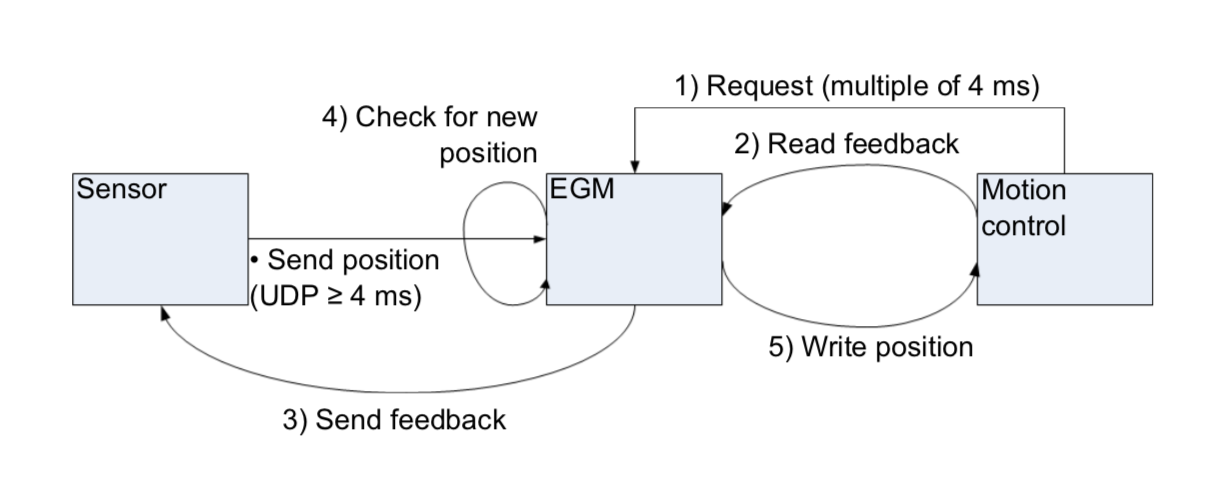
\includegraphics[width=11cm, height=5cm]{pic_endpoint-process-motion-diagram.png}
    \caption{The process that starts when EGMRunPose is called.}
    \label{fig:runpose_diagram}
\end{figure}

\begin{figure}[H]
    \begin{center}
    \tikzset{every picture/.append style={transform shape, scale=0.95}}
    \begin{sequencediagram}
    \renewcommand\unitfactor{0.5}
        \newthread{rapid}{\scriptsize{ : RAPID Program}}{}
        \newinst{rob1}{\scriptsize{ROB\_1 : Motion Control}}{}
        \newinst{egm}{\scriptsize{egmProc : EGM Process}}{}
        \newthread{end}{\scriptsize{ : EGM Endpoint}}{}
\scriptsize{
        \begin{call}{rapid}{MoveL Home}{rob1}{return}
        \end{call}
        \begin{sdblock}{test\_UDP()}{}
        \mess{rapid}{EGMReset egmProc}{egm}
        
        \begin{messcall}{rapid}{EGMGetId egmProc}{egm}
            \begin{call}{rapid}{EGMGetState(egmProc)}{egm}{egmSt}
            \end{call}
            \begin{messcall}{rapid}{EGMSetupUC ROB\_1, "default", "endpoint\_address"}{egm}
            \end{messcall}
            \begin{sdblock}{runEGM()}{}
            \mess{rapid}{EGMActPose egmProc}{egm}
            \begin{messcall}{rapid}{EGMRunPose egmProc}{egm}
                \begin{callself}{egm}{EGMRunPose $\rightarrow$ loop start}{Convergence $\rightarrow$ loop stop} 
                    %\mess[1]{egm}{get state}{rob1}
                    %\mess[1]{rob1}{return state}{egm}
                    \begin{call}{egm}{get state}{rob1}{return state}
                    \end{call}
                    \setthreadbias{center}
                    %\mess[1]{egm}{send state}{end}
                    %\mess[1]{end}{return message}{egm}
                    \begin{call}{egm}{EgmRobot}{end}{EgmSensor}
                    \end{call}
                    \mess{egm}{write movement}{rob1}
                \end{callself}
            \end{messcall}
            \end{sdblock}
            \begin{call}{rapid}{EGMGetState(egmProc)}{egm}{egmSt}
            \end{call}
            \mess{rapid}{EGMReset egmProc}{egm}
        \end{messcall}
        \end{sdblock}
        %\mess{rapid}{}{egm}
}
        %\begin{call}{A}{EgmRobot}{B}{EgmSensor}
        %\end{call}
    \end{sequencediagram}
    \end{center}
    \caption{Sequence diagram for EGM position guidance.}
    \label{fig:sequence_pos_guide}
\end{figure}

Finally, position guidance execution happens when the instruction 'EGMRunPose emgProc' is called. While running, the EGM process will: sample the state from the motion control process, send the state data to the EGM endpoint, and place any motion instructions it receives from the EGM endpoint into the motion control processes queue. \cite[Sec. 9.3.2.3]{ABB:controller_software} provides a good diagram of this process (see figure \ref{fig:runpose_diagram}). For context, it is important to note that in figure \ref{fig:runpose_diagram} the naming conventions are slightly different than the ones used in this paper. For this paper, the object labeled 'Sensor' is an EGM endpoint, the object labeled 'EGM' is an EGM process, and the object labeled 'Motion control' is the motion control process. Figure \ref{fig:runpose_diagram} also refers to reading and sending 'feedback' (steps 2 and 3) as well as sending and writing 'position' (steps 4 and 5). This paper has been referring to the data called 'feedback' and 'position' as 'state data' and 'movement instructions' respectively. While this change in naming convention does happen in the documentation, this paper will attempt to keep the naming conventions as consistent as possible. To tie everything together, see the position guidance sequence diagram in figure \ref{fig:sequence_pos_guide}. \par




%*******************************************************************


%*******************************************************************
% PATH CORRECTION --------------------------------------------------
%*******************************************************************
\subsection{RAPID for EGM path correction}
\label{sec:EGM:Rapid_Programs:corr}
Running an EGM process for path correction is similar to running a process for position streaming with a few deviations. Path correction requires different process parameters (see section \ref{sec:EGM:Process_Management}). For the sake of this example, assume the parameters in figure \ref{fig:pathcorr_config}.

\begin{figure}[H]
    \centering
    \footnotesize{
    \begin{tabular}{| l | c |}
    \hline
        \textbf{Parameter} & \textbf{Value} \\ \hline
        Name        &   pathCorr \\
        Level       &   Path   \\
        Do Not Restart After Motors Off & No    \\
        Return to Programmed Position when Stopped & No \\
        Default Ramp Time & 2   \\
        Default Proportional Position Gain & 5  \\
        Default Low Pass Filter Bandwidth & 20  \\ \hline
    \end{tabular}
    }
    \caption{The default EGM process configuration.}
    \label{fig:pathcorr_config}
\end{figure}

The general sequence of events in path correction is similar to those of position stream. Both EGM processes run during execution of a RAPID program path. They differ in the messages that the endpoint sends different message protocols depending on mode. In position streaming, EgmSensor messages are sent from the endpoint and disregarded by the controller. In path correction, the endpoint sends EgmSensorPathCorr messages to the controller which are not ignored. The EgmSensorPathCorr messages contain $y$ and $z$ values for a translation of the TCP in reference to a 'correction frame'. In figure \ref{fig:rapid_path_corr}, the EGM process 'egmProc' is setup for 'ROB\_1' with 'pathCorr' parameters and transmission protocol 'endpoint\_address' by the instruction 'EGMSetupUC'. The EGM process is then started with 'EGMActMove'. This begins the data stream to the endpoint. When the first move instruction is called (i.e. MolveL Home) the endpoint receives EgmRobot messages, but any EgmSensorPathCorr messages sent are ignored. When the EGM move instruction (EGMMoveL) is called, the robot controller begins to take the EgmSensorPathCorr into account. While executing one of these EGMMoveL instructions, The actual position of the TCP can be displaced in the $yz$-plane of the correction frame (see section \ref{sec:EGM:Modes:corr}). 

\lstset{language=RAPID}
\begin{figure}[H]
    \centering
    \begin{lstlisting}
! Example assumes the definition of the targets
CONST robtarget Home;
CONST robtarget T10;
CONST robtarget T20;
VAR egmident egmProc;
! The EGM path correction procedure
PROC runPathCorr()
    EGMGetId egmProc;
    EGMSetupUC ROB_1, egmProc, "pathCorr", "endpoint_address"\PathCorr;
    EGMActMove egmProc tool0.tFrame\SampleRate:=4;
    MoveL Home, v100, fine, tool0 \WObj:=wobj0;
    EGMMoveL egmProc, T10, v100, z10, tool0 \WObj:=wobj0;
    EGMMoveL egmProc, T20, v100, fine, tool0 \WObj:=wobj0;
    MoveL Home, v100, fine, tool0 \WObj:=wobj0;
    EGMReset egmProc;
ENDPROC
\end{lstlisting}
\caption{Example RAPID program for EGM path correction.}
\label{fig:rapid_path_corr}
\end{figure}

As illustrated in figure \ref{fig:how_to_path_corr}, in path correction the tool frame ($x^{\prime}$, $y^{\prime}$, $z^{\prime}$) is displaced in relation to the correction frame ($x^{\prime\prime}$, $y^{\prime\prime}$, $z^{\prime\prime}$). The correction frame is defined with its $x$-axis in the direction of the movement (from Home to Target\_10) and the $yz$-plane is defined in relation to the $z^{\prime}$-axis of the tool frame (see section \ref{sec:Tech_Back:Rob_Move:frames}). Figure \ref{fig:how_to_path_corr} shows the deviation of the TCP from the path. When EgmSensorPathCorr messages contain corrections ($y$, $z$) which are not $(0,0)$, the robot controller will attempt to position the TCP at those coordinates in the correction frame. The pink line labeled 'correction' shows the trajectory of the TCP from the point the corrections were received to the point where the corrected position was reached. Without any corrections (i.e. $y=0$, $z=0$ in EgmSensorPathCorr messages) the TCP will be at the origin of the correction frame for the entire movement (i.e. the TCP will follow the path). 

\begin{figure}[H]
 \begin{center}
    \tikzset{every picture/.append style={transform shape, scale=1.15}}
\tdplotsetmaincoords{70}{110}
\pgfmathsetmacro{\ptheta}{55}
%\pgfmathsetmacro{\ctheta}{90}
\pgfmathsetmacro{\pphi}{30}
\pgfmathsetmacro{\lamb}{0.95}
%\pgfmathsetmacro{\cphi}{60}
\begin{tikzpicture}[tdplot_main_coords]
    
    
    \draw[BrickRed,thick,->] (0,0,0) -- (3,0,0) node[anchor=north east]{$x$};
    \draw[OliveGreen,thick,->] (0,0,0) -- (0,3,0) node[anchor=north west]{$y$};
    \draw[Blue,thick,->] (0,0,0) -- (0,0,3) node[anchor=south]{$z$};
    \tdplotsetrotatedcoords{0}{0}{70}
    \coordinate (O) at (0,0,0);
    \coordinate (S) at (1.0,3.5,1.25);
    
    \tdplotsetcoord{P}{3.464}{\ptheta}{\pphi}
   
    
    \tdplotsetrotatedcoordsorigin{(P)}
    \draw[dashed,tdplot_rotated_coords] (2.5,0,0) -- (-3,0,0) node[anchor=east]{\tiny{Home}};
    \draw[tdplot_rotated_coords] (2.6,-0.5,0) + (30:.5) node{\tiny{Target\_10}};
    \draw[tdplot_rotated_coords] (0,0.5,0.7) + (45:.25) node{\tiny{TCP}};
    \draw[dashed,color=RubineRed,tdplot_rotated_coords] (0.0,{0.25*cos(deg(0*\lamb))+0.25},{0.25*cos(deg(0*\lamb))+0.25})
        \foreach \a in {0.0,-0.01,...,-3.0}
        { -- ({\a}, {0.25*cos(deg(\a*\lamb))+0.25}, {0.25*cos(deg(\a*\lamb))+0.25})}node[anchor=south]{\tiny{correction}};
    
    \draw[thin,tdplot_rotated_coords,->] (0,0.5,0.5) -- (0.25,0.5,0.5);
    \draw[tdplot_rotated_coords] (0.25,0.5,0.5) + (45:.12) node{\tiny{$x^\prime$}};
    \draw[thin,tdplot_rotated_coords,->] (0,0.5,0.5) -- (0,0.25,0.5);
    \draw[tdplot_rotated_coords] (0,0.25,0.5) + (180:.08) node{\tiny{$y^\prime$}};
    \draw[thin,tdplot_rotated_coords,->] (0,0.5,0.5) -- (0,0.5,0.25);
    \draw[tdplot_rotated_coords] (0,0.5,0.25) + (0:.15) node{\tiny{$z^\prime$}};
    
    %\draw[dashed,thin,tdplot_rotated_coords,->] (0,0,0) -- (0,0,-1) node[anchor=north]{$z^\prime$};
    
    \draw[thick,color=RubineRed,tdplot_rotated_coords,->] (0,0,0) -- (1,0,0) node[anchor=west]{\tiny{$x^{\prime\prime}$}};
    
    \draw[thick,color=Green,tdplot_rotated_coords,->] (0,0,0) -- (0,1,0) node[anchor=west]{\tiny{$y^{\prime\prime}$}};
    
    \draw[thick,color=Cerulean,tdplot_rotated_coords,->] (0,0,0) -- (0,0,1) node[anchor=south]{\tiny{$z^{\prime\prime}$}};
    
    %\node[anchor=east, tdplot_rotated_coords] at (0,0.5,0.5){\footnotesize{corr}};
\end{tikzpicture}
\end{center}
\caption{The position of the tool frame ($x^{\prime}$, $y^{\prime}$, $z^{\prime}$) in relation to the correction frame ($x^{\prime\prime}$, $y^{\prime\prime}$, $z^{\prime\prime}$).}
\label{fig:how_to_path_corr}
\end{figure}


%                                    _____
%                              _.--""     ""--._
%                          _.-"                 "-._
%                        .F                         Y.
%                      .F                             Y.
%                     /   ..___                 ___..   \
%                    F   /   | """""-------""""" |   \   Q
%                   F   F    (.-"""-.     .-"""-.)    Q   Q
%                  F   F    .'       `. .'       `.    Q   Q
%                 J   F    /|    o    | |    o    |\    Q   L
%                 |  J     .`.       .' `.       .'.     L  |
%                 |  F    ( " `-...-'(   )'-...-' " )    Q  |
%                 | |      `.    _.-' '-' `-._    .'      | |
%                 Y |        L .'             `. J        | J
%                  L|        Q'                 `F        |J
%                   Q        |                   |        J
%                    L       C                   D       J
%                     \      \  ---...____..---  /     _/
%                      `L .-' `.               .' `-. P
%                       |`L   (|`-.__     __.-'|)   J'|__
%                       |  `-._`-..__"""""__..-'_.-'  |  """..
%           _..--""-..-' `.    `-..__"""""__..-"    .'\       `-.
%        .-"         L     `-._      """""      _.-'   L  *****:::.
%      ."            |         ""--.........--""        Q  *****...L
%     /"""""--..     F    .-""-.      |\ \               L  ::::::::L
%    J  ("  /| J    J   .' _/\_ `.    |_\ \              |   L____...L
%    F ._) /"| F    |   |  >..<  |    | |\.'             |            Q
%   J-----..._J     F   `.==..==.'    |_|                Q             L
%   F              J      '-..-'      | |                `.             Q
%  J               F                  |_|                  Q             Q
% /               J                   | |                   L             L
% F           __ J                    |_|                    Q            Q
%J           `._\|                    | |                     L            L
%F              ""L      .-""-.       |_|       .-""-.         L           Q
%Q                |    .'  ..  `.     | |     .'  ..  `.       |.__   __..::
% L               |    |  (  )  |     |_|     |  (  )  |       |':::::::''' |
% Q               Q    `.  ''  .'     | |     `.  ''  .'       |            |
%  L               L     `-..-'       |_|       `-..-'         J.-.         |
%   Q            _..Q                                         J'  J   .  |  J
%    L   __....:::'' \                                        F  J   J  J._J
%     L::::''''       Q                                      J  (  _J._,"
%      L               `.                                    Q_  `"
%      |          ."`.   )                           __...--"" \
%      |          Q   "-'                          .'\          L
%      Q   L  L    L                              <   Q       ___Q
%       L  Q   Q    `.            ""bmw--""        \   L--""""    L
%        '_.`.  `.    )            J     Q          Q  Q           |
%         J   `-' `-.'.._         |       L          L  L          Q
%         F            F `.       F       |          Q  |           L
%        L""""""--..._|   F      J        Q           L  Q   ___..--'
%        |           F   |       |         L          '---"""       |
%        |           |  J        F          L                       Q
%        |           |  |       |           Q                        L
%        ."""""---.._|  |     `.F            L                       |
%         `"""----.___`.|     ._)            Q                       Q
%          L          ""       )             |                        L
%          |                   Q             L                        L
%          Q                    L             |                       |
%           L                    L            |                      J
%            Q                   Q            F                      F
%             L                  .L          J                      J
%              Q             _..:' `.        |                      |
%               `.    ___...::''.   `.       |                      |
%                 `::::::'''    J    :       Q                      F
%                .' ___        J    .:        L                    J
%               J"""   "".._  .    .:'       .'::...___            |
%              J            '/    .:'       J  `.'''::::........:::'Q
%             F                 .::'        L    `.     ''''''''    'L
%             L               .::'          :.     L__   __..---..-' Q
%             :.            .::'            `:.       """             L
%              ':.._  _...::''               `::                      |
%                `':::::''                     ::.                    |
%                                                ::.                  |
%             (c) 02/01 by Benjamin M. Weiland     `::.              J
%                                                    `'::..__   __..:'
%                                                       `'::::::::''
%       https://www.asciiart.eu/space/astronauts
%****************************************************************************
% FRAMEWORK DEVELOPMENT
%****************************************************************************
\chapter{EGM Framework Development}
\label{sec:Dev}

\section{Overview}
\label{sec:Dev:Overview}
While this project required much research of the required technologies, the main goal was to create artifacts that would make simulation of robot systems that manage movement via EGM based on sensors and other components. To that end, an EGM framework was developed in three development iterations. The first iteration consisted mostly of researching EGM and the technologies involved in EGM, but a proof of concept was also developed in tandem with the research (see section \ref{sec:Dev:I1}). The second iteration required some research but it involved much more coding and experimentation where the concepts from the first iteration were used to model plausible use-cases for EGM and sensors (see section \ref{sec:Dev:I2}). The third iteration was mostly focused on refactoring and organizing the working code from the second iteration and deleting the non-functional or superfluous code (see section \ref{sec:Dev:I3}). 

\section{Iteration 1: Research and Prototyping}
\label{sec:Dev:I1}
The two goals for the first stage of development were:
\begin{enumerate}
    \item Control a virtual robot via EGM with data from some sort of sensor.
    \item Research EGM and its technology dependencies.
\end{enumerate} 

The following sections describe the process of constructing the example EGM endpoint found in the \cite[Sec. 9.3.3]{ABB:controller_software} as well as the subsequent modifications made to the example that resulted in a proof of concept. The general knowledge accrued by research during this stage constitutes the bulk of the information presented in sections \ref{sec:Tech_Back} and \ref{sec:EGM}. The code for the proof of concept that was developed during this stage can be found at \cite{Greg:Sensor}. 
%*******************************************************************



\subsection{Following the instructions}
\label{sec:Dev:I1:instructions}
Even though it can be difficult at the start of a project to know where to start, ABB provides a convenient jumping off point in the EGM documentation \cite[Sec. 9.3.3]{ABB:controller_software}. Presented there is a list of instructions for building an EGM endpoint with .Net (see figure \ref{fig:egm_endpoint_instructions}). 

\begin{figure}[H]
    \centering
    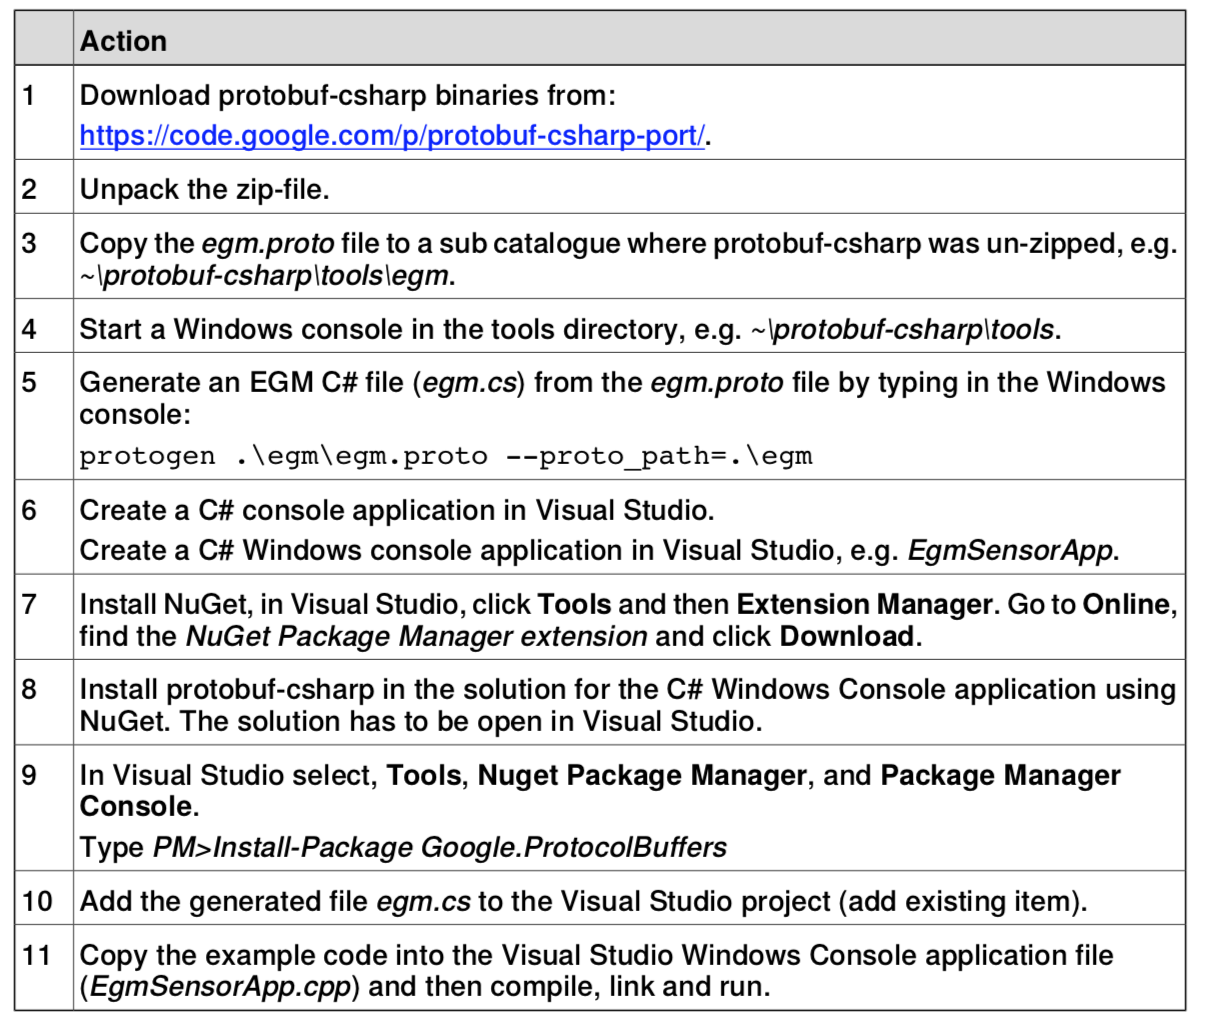
\includegraphics[width=11cm]{egm_endpoint_instructions.png}
    \caption{The instructions for a .Net egm endpoint.}
    \label{fig:egm_endpoint_instructions}
\end{figure}

While these instructions provided a starting point, there were some issues. The documentation suggests downloading the binaries for the protocol buffers from \cite{jskeet:github} and using them to compile the protocol definition file (egm.proto) into C\# code. While that method works, that link only has the binaries to compile protocol buffer files into C\# and C++ code. That is to say, when writing an endpoint in C\# or C++, steps 1-5 (in figure \ref{fig:egm_endpoint_instructions}) can be followed in order to compile C\# or C++ code from egm.proto. If, however, and endpoint needs to be written in another language, steps 1-5 will not work. To create an endpoint in python, the protocol buffer compiler for python will be needed. The binaries and source code for protocol buffer compilers version 2.6.1 for all languages can be found at \cite{Google:github}. This was the protocol buffer compiler version used during this project. The pre-compiled binaries from the link did not work when downloaded, however, building the binaries from the source code worked. Regardless of the method, at this point compiling egm.proto created a file called egm.cs. 

\subsection{Implementing the example EGM endpoint}
\label{sec:Dev:I1:ex_endpoint}
An example of an EGM endpoint written in C\# (egm-sensor.cs) is included with RobotStudio (see section \ref{sec:EGM:Endpoints} for file location). This file contains code that corresponds to the following pseudo-code:
%C:\Users\sas10gau\AppData\Local\ABB Industrial IT\Robotics IT\RobotWare\RobotWare_6.07.1011\utility\Template\EGM
\\
\\
\begin{algorithm}[H]
 \KwData{PORT = 8080, IPADDRESS = "localhost"}
 %\KwResult{how to write algorithm with \LaTeX2e }
 initialization of UDPserver at IPADDRESS on PORT\;
 \While{true}{
  UDPserver: wait to receive \emph{data}\;
  \eIf{data received}{
   EGMmessage $\leftarrow$ read from \emph{data} using egm.cs\;
   print some of EGMmessage\;
   make EGMresponse with dummy values \;
   send EGMresponse to origin address of EGMmessage \;
   }{
   print error message\;
  }
 }
 \caption{Pseudo-code of the contents of egm-sensor.cs}
\end{algorithm}
$$ $$
With the EGM message protocol compiled to a C\# serialization file (i.e. egm.proto $\rightarrow$ egm.cs as described in section \ref{sec:EGM:Message_Protos:message_v_protocol})  and a example of an egm endpoint in C\# (i.e. egm-sensor.cs) It was possible to implement and run the example endpoint. The steps taken to fully implement the example endpoint in Visual Studio are as follows:
\begin{enumerate}
    \item A visual studio console project called EGM-sensor was created. 
    \item The NuGet package manager was used to install the dependency called "Google.ProtocolBuffers" by JSkeet as per figure \ref{fig:egm_endpoint_instructions} instructions. (see \ref{fig:gpb_nuget} for package details)
    \item The serialization file (egm.cs) was added into the EGM-sensor project.
    \item The code from egm-sensor.cs was used in the main method of EGM-sensor. 
    \item The EGM-sensor project was built.
\end{enumerate}
Once built, running the EGM-sensor as a console app created a very basic EGM endpoint for position streaming. Testing the endpoint with robot controller running EGM was the next step. 


\subsection{Setting up RobotStudio for EGM}
\label{sec:Dev:I1:RobotStudio_setup}
With the basic EGM endpoint from section \ref{sec:Dev:I1:ex_endpoint} in place, RobotStudio was used to simulate a virtual controller to run EGM. For general information on configuring a robot controller for EGM, see section \ref{sec:EGM:Process_Management}. To configure a virtual controller in RobotStudio for EGM, the following steps were taken:
%controller -> Virtual Controller -> Change Options -> System Options -> Engineering Tools -> Check the EGM options
\begin{enumerate}
    \item \textbf{Create a new station}
    \item \textbf{Add a robot and controller to the station:} Home $\rightarrow$ Robot system $\rightarrow$ New system $\rightarrow$ Choose robot and robot controller
    \item \textbf{Enable the EGM RobotWare-option:} Controller $\rightarrow$ Virtual Controller $\rightarrow$ Change Options $\rightarrow$ System Options $\rightarrow$ Engineering Tools $\rightarrow$ Check 'Externally Guided Motion' (see figure \ref{fig:egm_option_enable})
    \item \textbf{Restart the controller to enable the option change}
    \item \textbf{Define an EGM Transmission Protocol:} Controller $\rightarrow$ Configuration $\rightarrow$ Communication $\rightarrow$ Transmission Protocol $\rightarrow$ Add new protocol (see figure \ref{fig:egm_trans_proto})
    \item \textbf{Define an EGM Process:} Controller $\rightarrow$ Virtual Controller $\rightarrow$ Change Options $\rightarrow$ Motion $\rightarrow$ External Motion Interface $\rightarrow$ Edit the 'default' or add a new process (see figure \ref{fig:egm_process_parameters})
    \item \textbf{Create a path for the robot} (see section \ref{sec:EGM:Rapid_Programs:stream} for example path)
    \item \textbf{Use the rapid editor to setup an EGM process} (see section \ref{sec:EGM:Rapid_Programs} for code examples)
        
    \item \textbf{Apply RAPID code to controller}
    \item \textbf{Run the simulation}
\end{enumerate}



\subsection{Connecting to the example EGM endpoint}
\label{sec:Dev:I1:conn_endpoint}
Once RobotStudio was setup according to the steps in section \ref{sec:Dev:I1:RobotStudio_setup}, The EGM-sensor project was run as a console app from Visual Studio and the simulation was started from RobotStudio. Once the simulation started, the robot followed the path given and the endpoint printed out the sequence number and time stamp of every EGM message it received. While the example endpoint provided only accesses the sequence number and time stamp of messages sent by the EGM process, this console app was a functioning EGM endpoint for position streaming. The next step was to build endpoints for position guidance and path correction. Just using the ABB's example code for an endpoint left one major issue to solve before anything meaningful could be done with EGM. The example endpoint only extracted the sequence number and timestamp from the incoming messages and populated the outgoing messages with arbitrary values because position stream ignores them anyway. To use position guidance or path correction, the actual state data from the robot would have to be extracted from the messages and then used to send meaningful responses back. The next hurdle was to learn to work with Google Protocol Buffers. \\


\subsection{An endpoint for position guidance and path correction}
\label{sec:Dev:I1:guide_corr_endpoints}
Unlike position streaming, building an EGM endpoint for position guidance and path correction requires the endpoint to build EgmSensor and EgmSensorPathCorr messages with meaningful data. At first, the meaningful data was hard coded into the endpoints. This worked well to test that the endpoints were communicating with the controller, but it soon became obvious that a way to change the data being sent to the controller in real-time was required. 

\subsection{Connecting a 'human sensor'}
\label{sec:Dev:I1:human_sensor}
When this project was proposed, the working title was "Simulation of Sensor Controlled Robotics". With the implementation of an EGM endpoint for position guidance, there was a proof of concept for control of a simulated robot. The nest step was to incorporate a sensor. The idea of a 'human sensor' originated with \cite{Castillo:YouTube} who implemented a graphical user interface (GUI) with sliders to interact with an EGM endpoint.\par

A GUI was built for each of the three different EGM endpoints (i.e. a different C\# form application was created to display and manipulate relevant data in the EGM endpoints). At this point, the focus shifted towards RobotStudio and experimenting with the components on the EGM process side of the EGM connection. These human sensors (PositionStreamForm.cs, PositionGuidenceForm.cs, and PathCorrectionForm.cs) were all bundled together with a controller (InactiveForm.cs) to make swapping between the endpoints easier. This bundle eventually was eventually built into a SmartComponent (discussed in section \ref{sec:Dev:I1:smart_comp}).



\subsection{Building the EGM endpoint into a SmartComponent}
\label{sec:Dev:I1:smart_comp}
It was expressed in discussions about the goals of the project that it would be useful to be able to use the EGM endpoints from within the RobotStudio simulation environment. If an endpoint was a simulated component, it would allow control of the endpoints from within the simulation (e.g. have the EGM endpoint start when the simulation is started). To accomplish this, the EGM endpoints were build into a smart component. The first step to build a smart component for RobotStudio is to download and install RobotStudio SDK (software development kit). The SDK is available at \cite{ABB:RS_SDK}. If Visual Studio is installed before the SDK is installed, the SDK installation will automatically include the template for smart components in Visual Studio. Instructions for building smart components can be found at \cite{ABB:Smart_Components}. By following these instructions, an EGM endpoint SmartComponent was built. The SmartComponent (EGM\_Server) code can be found at can be found at \cite{Greg:Sensor}. With this proof of concept complete, the second development iteration began with the goal to incorporate a virtual sensor.


\section{Iteration 2: Simulating Sensor Control}
\label{sec:Dev:I2}
At this point in the project, there was an existing smart component that could act as an EGM endpoint for all three modes. With the close of the first stage of development, the second stage began with discussions about how an EGM and sensor simulation framework would be used. In general, these discussions implied that the three main areas that an EGM framework could find application in were:
\begin{enumerate}
    \item In simulations of sensor guided motion.
    \item As an adapter for other protocols to EGM.
    \item In damping the learning curve for those new to EGM. 
\end{enumerate}
That is to say, the project began to explore possible ways for a framework to solve these general problems. 

\subsection{Simulation goal}
\label{sec:Dev:I2:demo_goal}
It had been clear from the beginning of the project that any eventual framework should support both a library of sensor types and connecting these sensors to an EGM endpoint (see section \ref{sec:Intro:Proj_Goals}). To explore solutions for this, a more specific problem was presented to solve. It was decided to simulate a simplified version of the sensor-helmet system (section \ref{sec:Intro:Prob_Description}) to give the development of the framework a direction. Specifically, the goal was to simulate line sensors on the inside of a camera-helmet that was attached a robot arm (see figure \ref{fig:demo_model}). The sensors in the helmet would detect the position of the a 'head' and guide the motion of the robot via EGM. This development iteration was focused on demonstrating a simulation of collecting position data of a moving 'head' (sphere), and guiding the motion of the robot based on that data. Sensing the  orientation was also discussed, but time constraints lead to a focus on position only. \par
 
 \subsection{An EGM line sensor}
 \label{sec:Dev:I2:egm_line_sensor}
The researchers were using line sensors mounted on the inside of a helmet to detect the position of the head. Coincidentally, one of the example smart components that ABB provides is a line sensor (download at \cite{ABB:Line_Sensor}). That line sensor SmartComponent was initially used in simulations. As the project progressed, the line sensor's functionality was expanded to include communicating its data to an EGM endpoint. 

\subsection{EGM sensor library prototype} 
\label{sec:Dev:I2:sensor_lib_prototype}
One of the goals of this project was to prototype a sensor library for use in EGM simulations. Time constraints prohibited the development of more than one EGM sensor for the library prototype. That is to say, of the several configurations of an EGM compatible line sensor that were explored during this iteration, the configuration that was found to be most widely applicable became the prototype of the sensor library. EgmLineSensor.cs (the final configuration) is discussed in section \ref{sec:Result:LthRobotStudio}, but its development lead to the formulation of several general principles that might be helpful when developing future EGM sensors:
\begin{enumerate}
\item Define a complete and unique message protocol for each sensor type.
    \begin{itemize}
        \item It is possible to send sensor data without a message protocol, but doing so can lead to problems interpreting the data.
        \item It is possible to piggy-back the sensor data into an existing message protocol, but doing so can cause unnecessary complexity.
    \end{itemize}
\item Include SmartComponent properties for unique identification (sensor ID) and message addressing (port number). 
    \begin{itemize}
        \item Making adding a sensor ID and a port number property to the smart component xml file (see section \ref{sec:Result:LthRobotStudio:EgmLineSensor}) allow these things to be changed in RobotStudio without building and importing a new version of the smart component. 
    \end{itemize}
\item The message protocol should include a field for all the sensor data and for the sensor ID. 
\end{enumerate}

\subsection{The need for adapters}
\label{sec:Dev:I2:adapters}
The second possible use of an EGM framework that was discussed was to build adapters. Rather, it is more accurate to say that the name 'adapter' was used to describe several similar types of EGM endpoint that were discussed. Another area of research in the robotics lab (at the time of writing) involved developing "[a] bridging framework [which] exposes the ABB externally guided motion research interface (EGMRI) low-level robot motion correction interface to the Julia language and other entities, such as Python and ROS" \cite{LU:egmri}. One constraint to this research that was expressed in relation to this project was that EGMRI is only supported on the controller of ABB's YuMi robot. To ease this constraint it was suggested that EGMRI could be implemented for virtual robots in RobotStudio with a combination of appropriate virtual sensors (torque sensors) and an EGM endpoint that could translate from the EGMRI message protocols to EGM message protocols. It was also suggested that being able to develop EGM and EGMRI applications in other programming languages (like the aforementioned, Python) could be useful.  

\subsection{An EGM adapter for python}
\label{sec:Dev:I2:python_adapter}
When discussing an adapter framework and its applications, there were two constituent concepts that were explored at this point. I.e. adapting another message protocol to the EGM message protocol and the use of EGM in an application written in Python. It was thought that the best way to explore these concepts while implementing a simulation of the sensor-helmet was to have an EGM endpoint that would communicate with both the robot controller (via EGM) and a python script (via a new protocol). The idea was that the endpoint would store all incoming state date from the robot and it would have a persistent 'next target' that it would constantly send to the robot controller as movement instructions. The Python script would be able to send updates of the next target as well as request current state data from the endpoint. When line sensors would send position data to the Python script, it would calculate and update the required next target from the sensor data and from the robot state data it had. That is, the goal was to develop the following components to use EGM to follow a moving ball:
\begin{enumerate}
    \item An EGM line sensor to gather and send distance data.
    \item A message protocol for the line sensor.
    \item A message protocol to for managing the next target
    \item A Python script to:
        \begin{enumerate}
            \item Receive sensor protocol messages.
            \item Send and receive next target messages.
            \item Calculate the next target.
        \end{enumerate}
    \item An EGM adapter (endpoint) to:
        \begin{enumerate}
            \item Manage EGM communication (via EgmRobot and EgmSensor messages).
            \item Manage next target communication with the Python script.
        \end{enumerate}
\end{enumerate}
These goals were achieved in the sense that: all of the components were implemented, the correct data arrived at the intended components, the protocol messages were deserialized correctly, and the motion of the robot was affected by the system. There were, however, latency issues that were severe enough to render the system unusable. A diagram of the result can be seen in figure \ref{fig:python_adapter} below, with the corresponding code available in the repositories  \~/Test\_Ex.cs/Program.cs in \cite{Greg:LTH_EGM} and \~/Notebooks/Adapter.ipynb in \cite{Greg:Jupyter}. Currently, the code in Program.cs that was used for this configuration is commented out in favor of a configuration that worked. 

\begin{figure}[H]
    \centering
    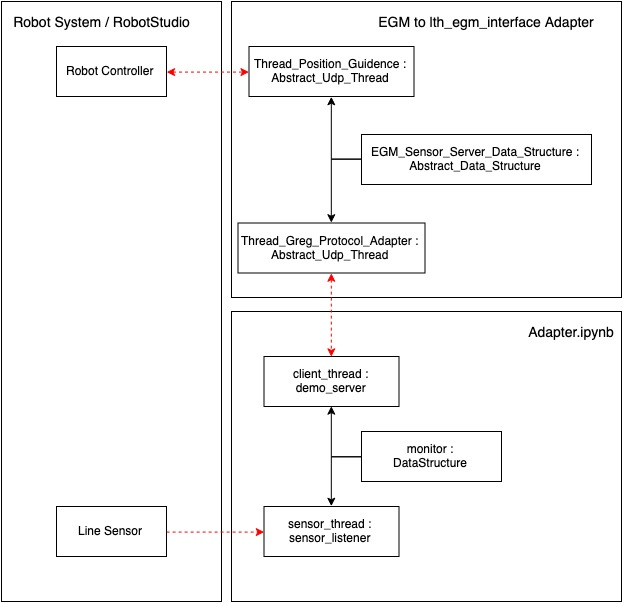
\includegraphics[width=10cm]{python_adapter.jpg}
    \caption{An exploration of python.}
    \label{fig:python_adapter}
\end{figure}
The details of the Python-adapter system will not be discussed any further in this paper because, at this point in the project, the decision was made to stop pursuing a demonstration in this configuration. What insight was gleaned into the concepts of adapters and EGM in Python is revisited in appendix \ref{app:Hypothetical:python}, but development along these lines stopped here. It was thought that an adapter was unnecessary for the purposes of a demonstration and it was hoped that the latency issues could be avoided by simplifying the system to a single EGM endpoint written in C\#. 

\subsection{A single EGM endpoint in C\#}
\label{sec:Dev:I2:one_endpoint}
Changing the configuration to a single endpoint in C\# did not fix the latency issues. A video of the demonstration at this stage of development can be found at \cite{Greg:Bad_Demo}. Although this particular video was recorded when the project direction had completely turned away from adapters and Python scripts, the gradual slowing down and then erratic movements seen in the video are essentially identical to the latency issues of the Python-adapter configuration. It was concluded that the issue had to be with how UDP was being handled by the threads.


\subsection{Damping the learning curve for new users of EGM}
\label{sec:Dev:I2:fixing_udp_thread}
After some experimentation with the UDP thread algorithm, the cause of the latency issues became apparent. The example UDP thread provided by ABB (see section \ref{sec:Dev:I1:ex_endpoint}) is not periodic. The model for the example thread was to call a blocking receive function on the UDP socket, then let the thread be blocked until an EgmRobot message arrived in the buffer. This algorithm was abandoned very early in development because it made it impossible to exit and close the thread safely. If the EGM endpoint is being run from a terminal application (like the example was) this is not an issue. If a thread of this type is being run from within a smart component that is being simulated, this causes problems. If the thread is blocked waiting for an EgmRobot message within the simulation, and the simulation stops while the thread is still blocked, RobotStudio crashes. The solution to this issue was to make the threads periodic and make the receive calls non-blocking. Introducing line sensors into the system increased the volume of UDP messages past the point that the periodic threads could handle them. By logging the sequence numbers and timestamps of the EGM protocol messages, it became clear that that messages were not being handled quickly enough. This resulted in backups in the UDP buffers. If left running, the backup would cause messages to be handled later and later until there was buffer overflow and packets were lost. In the video, this can be seen clearly from the behavior of the robot. As the simulation progresses, the robot responses become more delayed as the buffers backup until the movements become erratic as the buffers overflow. After some experimentation, a solution to this problem was found (see algorithm \ref{alg:egm_udp_thread}). 
\begin{algorithm}[H]
\label{alg:egm_udp_thread}
 \KwData{portNumber, monitor, sleepTime, defaultSleep}
 %\KwResult{how to write algorithm with \LaTeX2e }
 Create a socket on localhost\;
 Bind socket to portNumber\;
 \While{runThread}{
  \eIf{socket has data}{
    receive \emph{data}\;
    handle \emph{data}\;
    sleepTime = 0\;
   }{
    sleepTime = defaultSleep\;
  }
  make \emph{returnMessage} if needed\;
  \If{returnMessage not null}
  {
     send returnData via socket\;
  }
  sleep thread for \emph{sleepTime}
   
 }
 \caption{Algorithm for handling UDP communication.}
\end{algorithm}
$$ $$
The solution of making the UDP threads check the buffer for data periodically but executing again immediately if it had just received data prevented the backups and overflows. Using this model, the simulated sensor-helmet system worked well. 

\section{Iteration 3: Designing Generalized Tools}
\label{sec:Dev:I3}
The third iteration started with the successful implementation of a simulated solution for tracking the motion of a ball with a sensor, and then following that motion with a robot based on that sensor data. The issue to address at this stage was not if the sensor-helmet could be simulated, but if the simulation components could be generalized into useful simulation tools. The tools that were developed during this iteration are presented in section \ref{sec:Result}, but there were three main design principles that were followed in this iteration:
\begin{enumerate}
    \item Provide a working general-purpose UDP thread.
    \item Concentrate the program logic in as few places as possible.
    \item Additions to the framework or sensor library should not require updating any RobotStudio binary files (i.e. additions should be able to be self contained).
\end{enumerate}
Using the tools that were developed in this iteration, a second simulation of the sensor-helmet system (see section \ref{sec:Intro:Prob_Description}) was built. A video of this simulation can be found at \cite{Greg:Demo}.

%
%
%
%
%
%
%
%              _
%             | |
%             | |===( )   //////
%             |_|   |||  | o o|
%                    ||| ( c  )                  ____
%                     ||| \= /                  ||   \_
%                      ||||||                   ||     |
%                      ||||||                ...||__/|-"
%                      ||||||             __|________|__
%                        |||             |______________|
%                        |||             || ||      || ||
%                        |||             || ||      || ||
%------------------------|||-------------||-||------||-||-------
%                        |__>            || ||      || ||
%
%
%     hit any key to continue
%
%          https://www.asciiart.eu/computers/other
%****************************************************************************
% RESULT
%****************************************************************************
\chapter{Result}
\label{sec:Result}

\section{Overview}
\label{sec:Result:Overview}
The result of the final development iteration (LthRobotStudio) will discussed in detail here. The LthRobotStudio code repository can be found at \cite{Greg:LthRobotStudio}. Over the course of this project, many different ways to use EGM were explored. Regardless of the specific application of EGM, every design iteration consistently required addressing the following considerations:
\begin{itemize}
    \item Sending and receiving data via UDP.
    \item Serializing and deserializing Google Protocol Buffer messages.
    \item Defining logic for reading and writing Google Protocol Buffer messages.
\end{itemize}
Of these considerations, only the third required major code changes for each new experiment. The first required only a few minor changes and the second is completely handled by the code generated by Google Protocol Buffers. The contents of LthRobotStudio are an attempt to consolidate and abstract the constants while leaving the variables open. There implementation used for the project demonstration are also included for reference as well as a prototype sensor.

\section{The Final Product: LthRobotStudio}
\label{sec:Result:LthRobotStudio}
There are four namespaces in LthRobotStudio: EgmFramework, EgmMessageProtocols, EgmLineSensor, and EgmEndpoint. The relevant architecture components can be seen in figure \ref{fig:LthRobotStudio}. It is important to note that details have been omitted in the diagram so as not to overwhelm the relevant information. Discussions of the omitted details are included in the sections discussing the namespaces.
\begin{figure}[H]
    \centering
    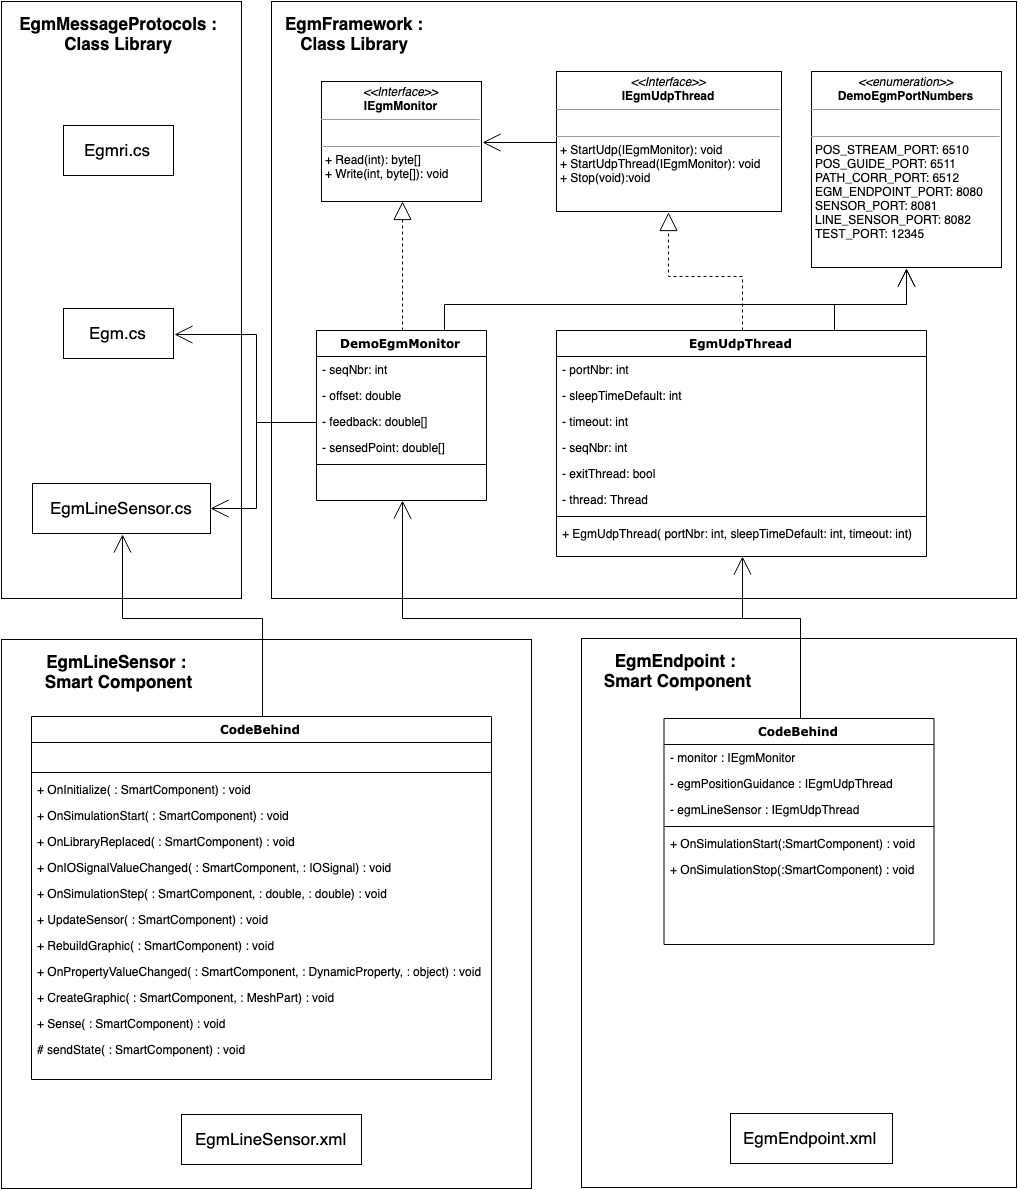
\includegraphics[width=12cm]{LthRobotStudio.jpg}
    \caption{The current architecture of LthRobotStudio.}
    \label{fig:LthRobotStudio}
\end{figure}

\subsection{EgmFramework}
\label{sec:Result:LthRobotStudio:EgmFramework}
The EgmFramework namespace is responsible for synchronous communication and program logic. This is the only section where the class diagram in figure \ref{fig:LthRobotStudio} is not omitting details. Because the EGM interface assumes UDP-based synchronous communication between the EGM process in the robot controller and the EGM endpoint, it follows that a simple way to create a larger application based around an EGM endpoint is to apply the same concurrent programming principle already expected by the robot controller to the rest of the system (I.e. use UDP for all communication because its used by ABB already). The EgmFramework uses two main concepts to support a larger system: a monitor, and a UDP thread. The intent of a UDP thread is to receive and send UDP messages only. The logic of what to do with incoming messages and what messages to send out is intended to be defined by the user inside of a monitor. The interfaces IEgmMonitor and IEgmUdpThread define the methods required to implement these two concepts.\par

EgmUdpThread is an implementation of IEgmUdpThread. An instance of EgmUdpThread is a wrapper class for a UDP server thread that contains an IEgmMonitor. The method StartUdpThread() contains the thread logic (i.e. the UDP server). When the method StartUdp() is called, a worker thread is created using the method StartUdpThread(). When the method Stop() is called, the currently running thread is stopped and shut down safely. For details of the how the thread handles UDP communication, see section \ref{sec:Dev:I2:fixing_udp_thread}. The important detail is that on every iteration of the main loop, the UDP thread will:
\begin{itemize}
    \item Try to get raw data from its buffer.
    \item Try to pass any raw data it was able to get to its monitor by calling the method Write(portNbr, data).
    \item Try to get response data from the monitor by calling the method Read(portNbr).
    \item Try to send response data to address of last sender.
\end{itemize}
The constructor for EgmUdpThread accepts three parameters: a port number, a default wait time, and a timeout time. The port number is, obviously, the port on which the UDP thread will listen for messages. The assumption is that any system built with the framework will use the port numbers of the UDP threads for addressing communications as well as for managing the program logic in the monitor (see appendix \ref{app:Code:DemoEgmMonitor} for examples). The default wait time is used by the thread to define how often it should check for new data if there is no data currently. That is to say, if there is no data in the buffer when the thread checks it, a default sleep time of 5 will cause the thread to sleep for 5 $ms$ before running the main loop again (i.e. checking the buffer for data again). If there is data in the buffer, the thread will run the main loop again without sleeping. There are two factors that lead to this design decision:
\begin{enumerate}
    \item one possible source of data loss in UDP is buffer overflow, therefore if there is data in the buffer it must be read as fast as possible or risk loosing newer packets.
    \item The robot controller performs EGM operations periodically (every 4 $ms$ at fastest). Being able to set a wait time for the UDP thread allows other threads to execute in the dead time while not blocking the thread on the condition of receiving data. 
\end{enumerate}
That is all to say, the UDP threads are designed to be pseudoperiodic in order to be able to minimize the risk of loosing UDP packets while at the same time not wasting processor resources which reduces the risk of scheduling issues. \par

The class DemoEgmMonitor is an implementation of the IEgmMonitor interface. The intended use of the framework is that the user will implement their own IEgmMonitor. DemoEgmMonitor is the monitor used to build the demonstration fo this project. It has been left in the framework as an example. The process is intended to be:
\begin{enumerate}
    \item A UDP thread calls Write(portNbr, data).
    \item Based on the port number, the monitor deserializes the data into the correct Google Protocol Buffer message.
    \item The message is used in some user defined way (e.g. parameters saved, calculations done, etc.)
    \item A UDP thread calls Read(portNbr).
    \item Based on the port number, the monitor creates the correct Google Protocol Buffer message, serializes it, and returns the data to the calling UDP thread.
\end{enumerate}
In the DemoEgmMonitor, these operations are accomplished by a switch case on the port number given in each method. \par

The last member of the EgmFramework namespace is the enumeration called DemoEgmPortNumbers. There is not much to discuss with this class. It is an artifact of the development process and was used at one point to organize the different port numbers that were in use. Early in development, the addressing of the different threads was done as a parameter within different unique thread classes and having a global address list was useful. As the framework design evolved, the program logic was broken out of the UDP thread, and instead of many different thread classes with hard coded port numbers, assigning a port number to a thread was done in the constructor of a single generic UDP thread class (EgmUdpThread). DemoEgmPortNumbers has not been removed because having a global port number definition makes example code slightly easier to follow. 

\subsection{EgmMessageProtocols}
\label{sec:Result:LthRobotStudio:EgmMessageProtocols}
This namespace is has the most detail omitted. The code in this namespace was automatically generated from Google Protocol Buffer message definition files. The classes in EgmMessageProtocols are responsible for serializing and deserializing messages. The classes and methods are omitted in the diagram because the it is more useful to describe the structure of the protocol messages and to give practical usage examples.\par

Egm.cs handles serializing and deserializing EgmRobot, EgmSensor, and EgmSensorPathCorr messages (discussed at length in section \ref{sec:EGM:Message_Protos:proto_struct}). \par

Egmri.cs handles the messages for the externally guided motion research interface (EGMRI). Speciffically working with the EGMRI protocol has not been a priority in this project, but building simulations using EGMRI instead of EGM  has been discussed as a possible application for the framework. \cite{LU:egmri} discusses the protocol in more detail, but the main difference in the structure of the EGMRI and EGM protocol messages is that the state data that the robot controller sends to an endpoint includes the torque of the robot joints and the motion instructions that the endpoint sends to the robot controller include calibration parameters for a proportional-integral-derivative controller (PID controller). The serialization files for EGMRI have been included in case the framework will be developed further to support EGMRI in the future. \par

EgmLineSensor.cs is the serialization files for the message protocol used by the EgmLineSensor smart component namespace. The structure of the protocol can be found in figure \ref{fig:EgmLineSensorProto}. Following the same notation as in figure \ref{fig:egm_proto}, the $-$ symbol denotes that the field is required. 
\begin{figure}[H]
    \centering
    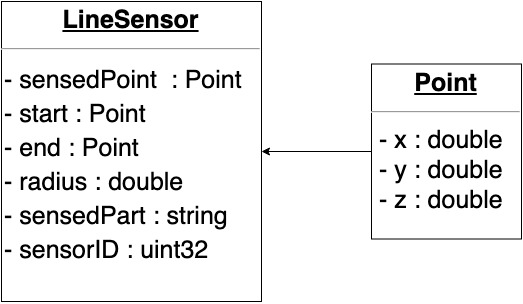
\includegraphics[width=5cm]{EgmLineSensorProto.jpg}
    \caption{The message structure for the EgmLineSensor protocol.}
    \label{fig:EgmLineSensorProto}
\end{figure}
The mechanics of a line sensor smart component will be discussed later in section \ref{sec:Result:LthRobotStudio:EgmLineSensor}, but for the purposes of the EgmMessageProtocols namespace, a LineSensor message is sent from a line sensor smart component that is in the RobotStudio simulation environment. This communication is intended to be one way (from the smart component to some UDP thread).

\subsection{EgmLineSensor}
\label{sec:Result:LthRobotStudio:EgmLineSensor}
The EgmLineSensor namespace contains the code for a line sensor smart component that supports one-way UDP communication of LineSensor protocol messages (section \ref{sec:Result:LthRobotStudio:EgmMessageProtocols}). Several properties were added to the EgmLineSensor SmartComponent in addition to the properties inherited from the Line Sensor SmartComponent \cite{ABB:Line_Sensor}. When imported into RobotStudio, a user can interact with the EgmLineSensor properties (as seen in \ref{fig:egm_line_sensor_properties}). The definitions of these properties can be found in the EgmSmartComponent.xml file (excerpt in figure \ref{fig:EgmLineSensorXml}). The properties 'End', 'Start', and 'Radius' define the dimentions of the sensor's detection range. The detection range is the cylinder of volume in which a simulated object will be detected by the EgmLineSensor. The 'SensedPart' and 'SensedPoint' properties are the string identifier and nearest point of an object that passes through the detection area. The 'SensorID' and 'PortNumber' properties are given by the user to define the destination of sensor data and a unique identifier for this sensor. The advantage of including a 'SensorID' along with the sensor data is that a single EgmUdpThread can receive sensor data from a number of sensors. 

\begin{figure}[H]
    \centering
    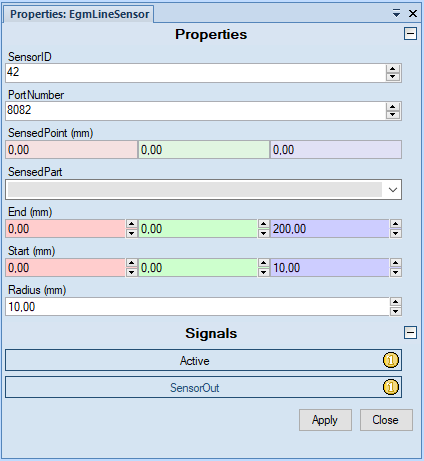
\includegraphics[width=6cm]{line_sensor_properties.png}
    \caption{EgmLineSensor properties as see from within RobotStudio.}
    \label{fig:egm_line_sensor_properties}
\end{figure}

On each simulation step, the EgmLineSensor calles the Sense() method. Sense() checks for any objects within the detection area and will then update the values of 'SensedPart' and 'SensedPoint'. When either the 'SensedPoint' or 'SensedPart' properties change during a simulation, the EgmLineSensor will call the sendState() method. The method will build a LineSensor message, serialize it using EgmLineSensor.cs and send the serialized message to the given port number. There is an excerpt of the EgmLineSensor CodeBehind.cs in figures \ref{fig:EgmLineSensorCodeBehind1} and \ref{fig:EgmLineSensorCodeBehind2} which shows the details of the sendState() method. \par

The details of the properties defined in EgmLineSensor.xml were omitted from the diagram in \ref{fig:LthRobotStudio} to avoid confusing the meaning of the class diagram notation. It was decided that the clearest way to present these properties was to include the xml excerpt and a picture of the SmartComponent properties GUI from within Robotstudio. \par




\subsection{EgmEndpoint}
\label{sec:Result:LthRobotStudio:EgmEndpoint}
The EgmEndpoint namespace contains the code for an EgmEndpoint SmartComponent. While there are some properties defined in the EgmEndpoint.xml file, these properties are defined by default as a part of the SmartComponent template in Visual Studio and were never used. Because they were never used they will not be discussed. The CodeBehind class in the EgmEndpoint namespace of figure \ref{fig:LthRobotStudio} omits several unused default SmartComponent methods. The OnSimulationStart() and OnSimulationStop() methods (see figure \ref{fig:EgmEndpointCodeBehind}) are included because they are used during simulations.\par

At the start of a simulation, calling the OnSimulationStart() method of EgmEndpoint will create an instance of the DemoEgmMonitor class (monitor) and two instances of EgmUdpThread (egmPositionGuidance on port 6511 and egmLineSensor on port 8082). EgmEndpoint will then call StartUdp() on both threads passing them both the monitor. At the end of the simulation, calling OnSimulationStop() method will call the Stop() methods of the EgmUdpThreads and then set references to the threads and monitor to null. Closing the threads like this prevents RobotStudio from throwing exceptions when the simulation is stopped. \par

It is important to note that this SmartComponent is an example of how the EgmFramework can be used to implement an EGM endpoint (see section \ref{sec:EGM:Endpoints}). Simulations of other sensor guided robot system will require implementing an EGM endpoint that is specific to that system. 



\section{Demonstration of Sensor Control Simulation}
\label{sec:Result:Demo}
To provide a concrete development goal, it was decided early in the project to use the tools developed to simulate a version of the sensor-helmet system described in section \ref{sec:Intro:Prob_Description}. A working simulation was achieved in the second development iteration and the lessons learned building that simulation were subsequently used in the third iteration to create the generalized tools in LthRobotStudio \cite{Greg:LthRobotStudio}. Although a video of a working simulation has been presented earlier in this paper, what follows is a cleaner video of only the simulation as well as an explanation of the interactions of the components used to create the simulation. As can be see in figure \ref{fig:demo_markup}, a sensor-helmet was created by attaching an EgmLineSensor smart component to a half-sphere body. The helmet was in turn attached to the TCP of a robot. A red sphere was used to represent a head in this simulation (using a 3d model of an actual head was found to be too disconcerting for the developer). The head was moved along the simulation's $y$-axis by employing a standard RobotStudio SmartComponent called a 'linear mover'. The EgmLineSensor was positioned on the concave surface of the helmet in such a way that its detection range runs parallel to the simulation's $y$-axis. 

\begin{figure}[H]
    \centering
    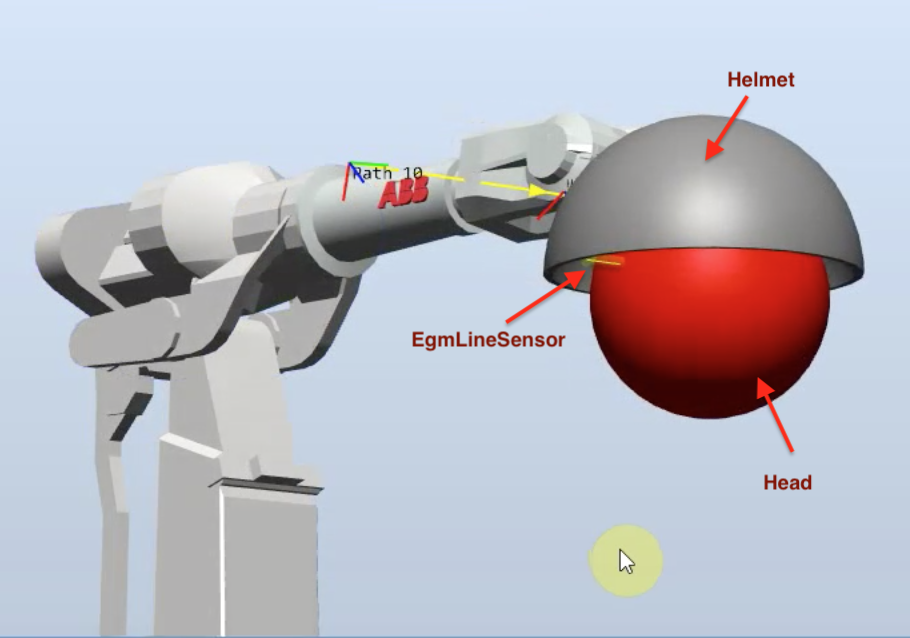
\includegraphics[width=11.5cm]{Demo_markup.png}
    \caption{Sensor-helmet simulation part labels.}
    \label{fig:demo_markup}
\end{figure}

The following communication events are all numbered as to correspond to the numbered communication lines in figure \ref{fig:demo_arch}. (1) The position of the head is detected by the EgmLineSensor. (2) The properties of the EgmLineSensor are set to send the LineSensor messages to port 8082. Also included in this simulation environment was an EgmEndpoint SmartComponent. As explained in section \ref{sec:Result:LthRobotStudio:EgmEndpoint}, the EgmEndpoint was built specifically for this demonstration. (2) It contains an EgmUdpThread called egmLineSensor bound to port 8082 which receives the serialized LineSensor messages from the EgmLineSensor and (3) passes them to the monitor (an instance of DemoEgmMonitor) by calling the Write() method. EgmEndpoint also contains another EgmUdpThread (bound to port 6511) called egmPositionGuidance which also has a reference to the monitor. An EGM process is started in the virtual controller by the RAPID program. (6b) This process's transmission protocol communicates with an EGM endpoint on port 6511. (4) When the EgmRobot messages arrive at egmPositionGuidance, they are passed to the monitor by calling the Write() method. The monitor uses the port number of the EgmUdpThread that calls Write() to decide what de-serialization protocol to use. If the calling thread is on port 8082, the monitor de-serializes the data as a LineSensor message (using EgmLineSensor.cs) and calculates the change in $y$ position ($\Delta y$) for the head based on the previous sensor data. If Write() is called by the thread on port 6511, the monitor deserializes the data as an EgmRobot message (using Egm.cs) and extracts the state data of the robot. When a thread on port 8082 calls the Read() method of the monitor null is returned, thereby causing the thread to send no response. (4) If Read() is called by a thread on port 6511, the monitor uses the $\Delta y$ and the current robot state data to calculate the required movement instruction for the robot. The monitor will then: build an EgmSensor message containing the movement instruction, serialize it using Egm.cs, and finally return the serialized EgmSensor message to the thread that called Read(). (6a)The serialized EgmSensor message will then be sent to the EGM process. (7) The EGM process then passes the movement instruction to the motion control process. The video of these concurrent processes can be viewed at \cite{Greg:Final_Demo}. 

\begin{figure}[H]
\vspace{2cm}
    \centering
    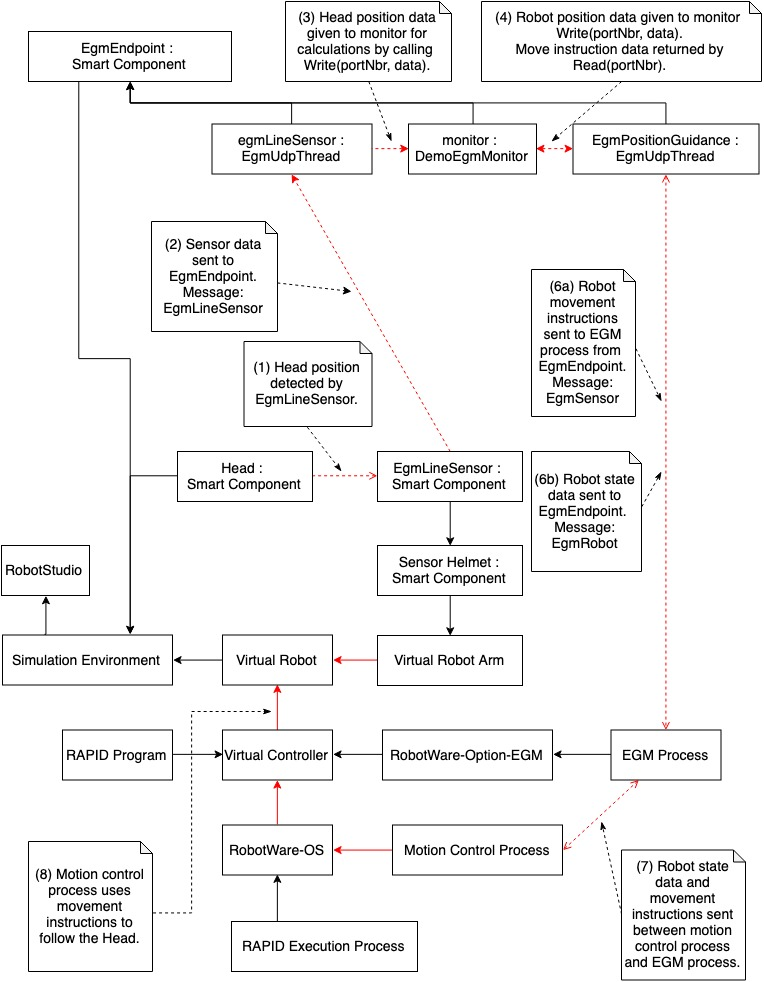
\includegraphics[width=14cm]{ArchComponents2.jpg}
    \caption{Entities in the demonstration. Data flow connections in red.}
    \label{fig:demo_arch}
\end{figure}



%                 .-.
%                (   )
%                 '-'
%                 J L
%                 | |
%                J   L
%                |   |
%               J     L
%             .-'.___.'-.
%            /___________\
%       _.-""'           `bmw._
%     .'                       `.
%   J                            `.
%  F                               L
% J                                 J
%J                                  `
%|                                   L
%|                                   |
%|                                   |
%|                                   J
%|                                    L
%|                                    |
%|             ,.___          ___....--._
%|           ,'     `""""""""'           `-._
%|          J           _____________________`-.
%|         F         .-'   `-88888-'    `Y8888b.`.
%|         |       .'         `P'         `88888b \
%|         |      J       #     L      #    q8888b L
%|         |      |             |           )8888D )
%|         J      \             J           d8888P P
%|          L      `.         .b.         ,88888P /
%|           `.      `-.___,o88888o.___,o88888P'.'
%|             `-.__________________________..-'
%|                                    |
%|         .-----.........____________J
%|       .' |       |      |       |
%|      J---|-----..|...___|_______|
%|      |   |       |      |       |
%|      Y---|-----..|...___|_______|
%|       `. |       |      |       |
%|         `'-------:....__|______.J
%|                                  |
% L___                              |
%     """----...______________....--'
%
% https://www.asciiart.eu/television/futurama
%
%       "My story is a lot like yours, only more interesting 'cause it involves robots."
%                                                               - Bender Bending Rodríguez
%
%*****************************************************************************************
% ANALYSIS AND CONCLUSIONS
%*****************************************************************************************
\chapter{Analysis and Conclusions}
\label{sec:Anal_Con}

\section{The Project Goals}
\label{sec:Anal_Con:Goals}
This project was exploratory in nature with the (admittedly vague) goals to:
\begin{enumerate}
    \item Enable scripted motion adjustment based on virtual sensing during simulation in RobotStudio.
    \item Prototype a library of virtual sensors.
    \item Create a guide for offline simulation of robot programs using sensors to control motion.
    \item Demonstrate a simulation of sensor-controlled motion. 
\end{enumerate}
In pursuit of these goals, several artifacts have been produced. EgmFramework and EgmMessageProtocols were developed to enable scripted motion based on virtual sensing within RobotStudio simulations. EgmLineSensor was developed to prototype a library of virtual sensors. This paper was written as both a report for the project, but also a guide to the tools and knowledge that were developed over the course of this project. EgmEndpoint was developed to demonstrate a simulation of sensor-controlled motion using the other artifacts of this project. All of these artifacts can be improved and further developed, but within the context of an undergraduate student project, these goals are considered met. 




\section{Ethical Reflection}
\label{sec:Anal_Con:Ethics_Ref}
There is not much to discuss concerning the ethical implications of this project on its immediate context. Realistically, the work done here might be used by a few people. It is likely that the only people who will ever know of this particular small (and very specific) contribution to the body of knowledge in robotics will not need the framework that has been developed. That is to say, hopefully this work will be useful to someone. In a greater context though, the ethical implications of this project (or rather projects like it) is not insignificant. Robots capable of making autonomous decisions about their own behavior based on sensory data from their environment has applications in many fields. For example, the demonstration for this project comes from research into the applications of sensor guided robotics in surgical procedures. Robots are used in the construction \cite{Ethics:Con}, medical \cite{Ethics:Med}, food service \cite{Ethics:Foo}, and mining \cite{Ethics:Min} industries to name a few. Improvements to robots can lead to improvements in the quality for the products of those industries. Conversely, improvements in robotics can lead to higher product output per worker in those same industries. When fewer workers are required to produce the same product, if demand does not keep pace with the increased supply capacity for that product, some workers will lose their jobs. That is to say, improvements in automation can directly lead to job loss. Finally, any discussion of the ethical implications of improvements in autonomous robotics would be incomplete without mentioning that there are military applications for those improvements \cite{Ethics:Mil}. That is not to say that improvements to autonomous robotics and the implicit military applications are necessarily ethically wrong. Such improvements could lead to a reduction in collateral damage. The ethics of technology and its military application is an extremely complex issue that is dramatically outside the scope of this paper, but there is one aspect to that larger discussion that can not go unmentioned: autonomous robotics are already being used to kill people and this research and research like it can be used to improve autonomous robotics.


\section{Further Research}
\label{sec:Anal_Con:Fur_Res}
There are several paths that further research could take:
\begin{itemize}
    \item Build several generic demonstrations for learning EGM.
    \item Expand the sensor library.
    \item Implement EGMRI support.
    \item Migrate an application built with the framework to a real robot. 
\end{itemize}
That is to say, further work on the framework could take several directions. If this framework is to be used by people that are unfamiliar with robotics (i.e. students) it might be useful to implement several different examples that demonstrate some of the features of the framework. To be at all useful, more sensor types must be implemented. Implementing an EGMRI adapter was not accomplished during this project, but such an adapter would be useful. It would also be extremely useful to know if this framework can actually be used for offline programming. As it is now, it can be used to simulate a sensor-controlled robot system, but can that simulation be migrated to an actual robot?\par

A more in-depth discussion of the first three research topics has been included in appendix \ref{app:Hypothetical}. The text and figures found there can be considered an outline of where the author of this paper would start work if tasked to pursue development in those directions. As for migrating a framework application to a physics robot controller, the author would enthusiastically suggest beginning the research by allocating a robot and a large supply of coffee to them. 




%                             .     @$* @$3
%                            '$Nueeed$$ed$$eeec$$
%         ,            4$Lze@*$C2$b* ed(he*rb$CC$*$bc@$r
%   /@ |~~            .e$$"W$$B$B$**  ^$  e""##d&$Bd$$$Nc. ..      @\/~\
%   \==|         4$kd*Cr$6F#"`  **   .*==      # '"**F#$I$b$*       |   I
%      |         d$5N@$$"   ....eu$$$$$$N$*$zbeuu     #$d$$$$b.     / @/
%     @/     . z$Ted*"$P zue$*9d$$$@#       W$e@B$$L.    "#@$E$b@N
%           #d$Id*P#  'Nd$$B$**"       .*,     "#*N$$b$c   $$$*$$c
%          .d#+C6J   @@$B$*"          -***-        "#$$$$c   *$$$#$u
%       ..u$l4@"^"zJ$7W*"              '*`            ^*$@$$$r "$$E$@B>
%       *@$l$P"+Rd$$N#"          *     /|\     *        '"$$$c.. &E$*b
%       z$ "*.  .Jz$"           ***   / | \   ***         '*@N$b   d**N
%     .z$JBR^bs@$$#          *   *   /  |  \   *  *         "$l*9N "bN$Nee
%    4$$.C*   dB@"          ***    _/  /^\  \_   ***         '$$$z> 3$b$$#
%     $"$e$  @*$"        *   *     \\^|   |^//    *   *        $$$u.^*$N$c
%    JPd$%  @@d"        ***        ***********       ***       '$Ni$  $EP$
%  :e$"*$  :et$          *         ***********        *         ^$$E  4$N$be
%  ')$ud"  @6$                                                   9$$   $*@$"
%   @F*$   *4P                       ./                          '$m#   .$$.
%u*""""""""""""h                     ##=====                    e#""""""""""#
%E +e       ue. N                 ___##_______                 4F e=c     z*c
%#e$@e.. ..z6+6d"                #*************/               ^*cBe$u.  .$$@
%   $ ^"""" 4F"  ze=eu              ********              z***hc ^"$ ""*"" $
%   $       ^F :*    3r                                  @"  e "b  $       $
% .e$        N $  'be$L...                            ...&be@F  $F $       9F
%4" $        $ $.  zm$*****h.                      ue""""*h6   J$" $       4%
%$  $        $ $$u5e" .     "k                    d"       #$bu$F  $       4F
%"N $        $ ^d%P  dF      $  .            .e   $     -c  "N$F  .$       4F
% #$$        $  $4*. "N.    zP  3r ..    ..  $c   *u     $  u$K$  4F       4L
%  ^N$e.     3  F$k*. "*C$$$# .z$" '$    4L  "$c. '#$eeedF  $$$9r JF       J$
%   $'"$$eu. 4  F3"K$ .e=*CB$$$$L .e$    '$bc.u$***hd6C""  4kF$4F $F     u@$F
%   $   '"*$*@u N'L$B*"z*""     "$F" 4k 4c '7$"      "*$eu 4'L$J" $   .e$*"4F
%   $      '"hC*$ "$#.P"          $me$"  #$*$       .  ^*INJL$"$  $e$$*#   4F
%   $         $b"h ".F     $"     ^F        $       9r   #L#$FJEd#C@"      4L
%  .$         $Jb   J"..  4b      uF        *k      J%    #c^ $" d$        4L
% :"$         $k9   $ $%4c $Bme.ze$         '*$+eee@*$"  :r$    @L$        4$
% $ $         $$Jr  $d" '$r "*==*"            "#**"" $r  4$3r  db$F        4F
% $c$         $'*F  $"   '$            /\            $    *(L  $$$F         k
% #i*e.       $ 4>  $  ue $         \`.||.'/         'L c  $$ .L$d         .$
%  "b."*e.    4 4   $  $%db=eL     `.<\||/>.'      e*+$/$r  $ '$"$       .d$$
%   $^#+cC*mu 4r4   4r:6@F  $$    -----++-----    <$. "N&N  F  $ $    ud$$* $
%   $    "*eJ"@L4   4k*3Ic.*"      .'`.      #*5.J$$..F  $ $ ue#2*"   $
%   $       "N."@r  4Fd" '$r        /.'||`.\        4$ '"N*d"  9.$#Ce*"     $
%   $         "e^"  'd" uz$%           \/           '$czr"k#"  4Pu@"        $
%******************************************************************************
% REFERENCES        https://www.asciiart.eu/books/lord-of-the-rings
%******************************************************************************
\newpage
\addcontentsline{toc}{chapter}{Bibliography}
\bibliographystyle{IEEEtran}
\bibliography{thesis}



%                          __....-------....__
%                    ..--'"                   "`-..
%                 .'"                              `.
%               :'                                   `,
%             .'                                       ".
%            :                                           :
%           :                                             b
%          d                                              `b
%          :                                               :
%          :                                               b
%         :                                                q
%         :                                                `:
%        :                                                  :
%       ,'                                                  :
%      :    _____                  _____                   p'
%      \,.-'     `-.            .-'     `-.                :
%      .'           `.        .'           `.              :
%     /               \      /               \            p'
%    :      @          ;    :      @          ;           :
%    |                 |    |                 |           :
%    :                 ;    :                 ;          ,:
%     \               /      \               /           p
%     /`.           .'        `.           .'           :
%    q_  `-._____.-.            `-._____.-'             :
%     /"-__     .""           "-.__                    :'
%    (_    ""-.'                   """---bmw           :
%      "._.-""                                        ,:
%     ,""                                             P
%   ."                                                :
%  "      _."      ."        ."        _...           :
% P     ."        "        .'        ,"####)          :
%:     ."       ."        /        ,'######'          :
%:     :       (        ,"        ,########:         ,:
% q    `.      '.       ,        :######,-'          :
% `:    b       q       :        '--''""             :
%  :     :      :       :        :                   :
%  :     :      `:      `.       ".                 :'
%  q_    :       :       :         )                :
%    ""'b`._   ,.`.____,' `._   _.'                 ,
%       |.__"""              """     _______.......',
%     ,'    """""""-----.------"""""""               :
%     :                 :                            :
%     :                 :                            :
%     :.__              :           ________.......,'
%         """"""""------'------""""""
%
%     https://www.asciiart.eu/television/futurama
%*******************************************************************
% YOUR APPENDICES ARE BAD AND YOU SHOULD FEEL BAD
%*******************************************************************

\begin{appendices}


%*********************************
% INSTALL
%*********************************
\chapter{Installation and Usage}
\label{app:Install_Use}

\section{Installing the Framework in RobotStudio 6.07}
\label{app:Install_Use:RobotStudio}
There are two ways to use the tools created in this project. The first is to build an EGM endpoint as an external program to RobotStudio. The second is to build the EGM endpoint into a SmartComponent and import it into the RobotStudio simulation. Both of these methods assume that a virtual sensor SmartComponent will also be used in the simulation. In order for SmartComponents in a RobotStudio simulation to have access to serialization files for their message protocols, the framework dependencies (.dll files) must be copied into the RobotStudio binary folders. There are two options for aquiring the framework dependencies:
\begin{enumerate}
    \item Download the pre-built .dll files from the project repository.
    \item Build the project in Visual Studio locally.
\end{enumerate}

\subsection{Download dependencies}
\label{app:Install_Use:RobotStudio:download}
The .dll files used in this project can be found at \cite{Greg:Ref_Repo} in the folder /EgmFramework\_Demo/dll files/. The files needed are: Google.ProtocolBuffers.dll, Google.ProtocolBuffers.Serialization.dll, EgmFramework.dll, and EgmMessgaeProtocols.dll. 

\subsection{Build dependencies locally}
\label{app:Install_Use:RobotStudio:build}
Building the dependencies locally requires installing several packages in Visual Studio. The RobotStudio SDK must be installed (available at \cite{ABB:RS_SDK}). The framework also requires the NETStandard.Library (2.0.3). The NETStandard.Library (2.0.3) is available via NuGet at \cite{Microsoft:DNet}. To build the framework dependencies for RobotStudio:
\begin{enumerate}
    \item Clone or copy the github repository at \cite{Greg:LthRobotStudio}
    \item Open the project in Visual Studio.
    \item Build the solution.
    \item Use the creaded .dll files:
        \begin{itemize}
            \item \url{C:\ Users\ <user>\ .nuget\ packages\ google.protocolbuffers\ 2.4.1.555\ tools\ Google.ProtocolBuffers.dll}
            \item \url{C:\ Users\ <user>\ .nuget\ packages\ google.protocolbuffers\ 2.4.1.555\ tools\ Google.ProtocolBuffers.Serialization.dll}
            \item \url{C:\ <path-to-repo>\ LthRobotStudio\ EgmFramework\ bin\ Debug\ netstandard2.0\ EgmFramework.dll}
            \item \url{C:\ <path-to-repo>\ LthRobotStudio\ EgmFramework\ bin\ Debug\ netstandard2.0\ EgmMessgaeProtocols.dll}
        \end{itemize}
\end{enumerate}

\subsection{Copy dependencies to RobotStudio}
\label{app:Install_Use:RobotStudio:copy_to_RS}
Copy the dependencies (i.e. the .dll files aquired in \ref{app:Install_Use:RobotStudio:download} or \ref{app:Install_Use:RobotStudio:build}) to the RobotStudio binary folders:
\begin{itemize}
    \item \url{C:\ Program Files (x86)\ ABB Industrial IT\ Robotics IT\ RobotStudio 6.07\ Bin}
    \item \url{C:\ Program Files (x86)\ ABB Industrial IT\ Robotics IT\ RobotStudio 6.07\ Bin64}
\end{itemize}

\section{Running the Sensor-helmet System Demonstration}
\label{app:Install_Use:Run_Demo}
The RobotStudio station (demo\_helm\_backup.rspag) that was used to simulate a sensor-helmet system can be found at \cite{Greg:Ref_Repo} in the folder /EgmFramework\_Demo/. Install the framework dependienceis in RobotStudio (appendix \ref{app:Install_Use:RobotStudio:copy_to_RS}). Download and open demo\_helm\_backup.rspag in RobotStudio. 


\section{Using the Framework to Make an EGM Endpoint}
\label{app:Install_Use:Endpoint_Framewrok}
This project created EGM endpoints in two ways: as self-contained programs external to RobotStudio and as SmartComponents simulated within RobotStudio. The advantage of self-contained program is that alterations to the program during development do not require RobotStudio to update constantly. In contrast, alterations to a SmartComponent require restarting RobotStudio and the virtual controller before changes to the SmartCompnent will be registered. The advantage of the SmartComponent EGM endpoint is that it can be packaged as part of the RobotStudio station. This example will describe the process of building an EGM endpoint as a SmartComponent. In this case, the SmartComponent is a wrapper for the EgmFramework components so they can be started and stopped from within the simulation environment. To build a self-contained program, follow these instructions but wrap the EgmFramework components in another executable (e.g. a console app).\par 

Assuming the framework dependencies are installed in RobotStudio (see appendix \ref{app:Install_Use:RobotStudio}), to make an EGM endpoint as a SmartComponent:
\begin{enumerate}
    \item Create new SmartComponent project in Visual Studio (see section \ref{sec:Dev:I1:smart_comp})
    \item Go to the project's xml file and change the 'canBeSimulated' flag to true in the SmartComponent tag (i.e. <SmartComponent ... canBeSimulated="true">)
    \item Create an implementation of the IEgmMonitor monitor interface that handles the data:
        \begin{itemize}
            \item Implement the Read() method so that Google Protocol Buffer messages are correctly parsed according to the port number (example figure \ref{fig:DemoEgmMonitor_Read1})
            \item Implement the Write() method so that the correct message is created for each port number (example in figure \ref{fig:DemoEgmMonitor_Write})
        \end{itemize}
    \item Go to the project's CodeBehind.cs file and overwrite at least one of the smart component methods so that it creates and starts an EgmUdpThread with the implementation of the IEgmMonitor. 
    \item Build the Visual Studio solution.
    \item  Import the smart component .rslib file into a RobotStudio station.
\end{enumerate}

\section{Known Issues}
\begin{enumerate}
    \item Installation attempts to install and run with RobotStudio versions other than 6.07 have been unsuccessful. The causes of the issues have not been discovered as of the time of writing.  
    \item Runing the simulation in demo\_helm\_backup.rspag the first time works well. Resetting and running the simulation again causes RobotStudio to throw an unknown state exception which forces a shutdown. The cause of this issue is unknown at the time of writing. 
\end{enumerate}

%*********************************
% END INSTALL
%*********************************

%*********************************
% CODE
%*********************************
\chapter{Large Code Excerpts}

\section{EgmLineSensor}
\label{app:Code:EgmLineSensor}
\label{app:Code}
\lstset{language=XML}
\begin{figure}[H]
    \centering
    \begin{lstlisting}[fontadjust]
<SmartComponent 
 name="EgmLineSensor" 
 icon="EgmLineSensor.png"
 codeBehind="EgmLineSensor.CodeBehind,EgmLineSensor.dll"
 canBeSimulated="true">
	
<Properties>
 <DynamicProperty name="SensorID" valueType="System.Int32" value="1">
  <Attribute key="Quantity" value="None"/>
 </DynamicProperty>
 <DynamicProperty name="PortNumber" valueType="System.Int32" value="1">
  <Attribute key="Quantity" value="None"/>
 </DynamicProperty>
 <DynamicProperty name="SensedPoint" valueType="ABB.Robotics.Math.Vector3" readOnly="true">
 <Attribute key="Quantity" value="Length"/>
 </DynamicProperty>
 <DynamicProperty name="SensedPart" valueType="ABB.Robotics.RobotStudio.Stations.Part" readOnly="true"/>
 <DynamicProperty name="End" valueType="ABB.Robotics.Math.Vector3" value="0,0,0.4">
  <Attribute key="Quantity" value="Length"/>
 </DynamicProperty>
 <DynamicProperty name="Start" valueType="ABB.Robotics.Math.Vector3">
  <Attribute key="Quantity" value="Length"/>
 </DynamicProperty>
 <DynamicProperty name="Radius" valueType="System.Double" value="0.02">
  <Attribute key="Quantity" value="Length"/>
  <Attribute key="MinValue" value="0"/>
  <Attribute key="MaxValue" value="0.1"/>
  <Attribute key="Slider" value="true"/>
 </DynamicProperty>
</Properties>
    \end{lstlisting}
    \caption{Important parts of EgmLineSensor.xml.}
    \label{fig:EgmLineSensorXml}
\end{figure}

\lstset{language=[Sharp]C}
\begin{figure}[H]
\centering
\begin{lstlisting}[fontadjust]
protected void sendState(SmartComponent component){
    int PORT = (int)component.Properties["PortNumber"].Value;
    using (var sock = new UdpClient())
    {
        LineSensor.Builder sensorData = LineSensor.CreateBuilder();
        // #1 Code cut: see figure caption for ref to excerpt
        UInt32 sensorIDProperty = Convert.ToUInt32(component.Properties["SensorID"].Value);
        Vector3 sensedPointProperty = (Vector3)component.Properties["SensedPoint"].Value;
        String sensedPartProperty = Convert.ToString(component.Properties["SensedPart"].Value);
        Vector3 startProperty = (Vector3)component.Properties["Start"].Value;
        Vector3 endProperty = (Vector3)component.Properties["End"].Value;
        double radiusProperty = (double)component.Properties["Radius"].Value;
        // convert point from m to mm 
        sensedPointProperty = sensedPointProperty.Multiply(1000);
        // #2 Code cut: see figure caption for ref to excerpt
        LineSensor data = sensorData.Build();
        using (MemoryStream memoryStream = new MemoryStream())
        {
            data.WriteTo(memoryStream);
            var bytesSent = sock.SendAsync(
                memoryStream.ToArray(), (int)memoryStream.Length,
                "localhost", PORT);
        }
    }
}
\end{lstlisting}
\caption{sendState() method of EgmLineSensor.CodeBehind.cs (cut code \#1 and \#2 in figure \ref{fig:EgmLineSensorCodeBehind2})}
\label{fig:EgmLineSensorCodeBehind1}
\end{figure}

\lstset{language=[Sharp]C}
\begin{figure}[H]
\centering
\begin{lstlisting}[fontadjust]
// #1 Code excerpt: see figure caption for ref to parent code
Point.Builder sensedPoint = new Point.Builder();
Point.Builder start = new Point.Builder();
Point.Builder end = new Point.Builder();

// #2 Code excerpt: see figure caption for ref to parent code
sensedPoint.SetX(sensedPointProperty.x)
    .SetY(sensedPointProperty.y)
    .SetZ(sensedPointProperty.z);
start.SetX(startProperty.x)
    .SetY(startProperty.y)
    .SetZ(startProperty.z);
end.SetX(endProperty.x)
    .SetY(endProperty.y)
    .SetZ(endProperty.z);
sensorData.SetSensedPoint(sensedPoint)
    .SetStart(start)
    .SetEnd(end)
    .SetRadius(radiusProperty)
    .SetSensedPart(sensedPartProperty)
    .SetSensorID(sensorIDProperty);
\end{lstlisting}
\caption{Code excerpt from EgmLineSensor.CodeBehind.cs (sendState() method).}
\label{fig:EgmLineSensorCodeBehind2}
\end{figure}

\section{EgmEndpoint}
\label{app:Code:EgmEndpoint}
\lstset{language=[Sharp]C}
\begin{figure}[H]
    \centering
    \begin{lstlisting}[fontadjust]
public class CodeBehind : SmartComponentCodeBehind
{
    IEgmMonitor monitor = null;
    IEgmUdpThread egmPositionGuidance = null;
    IEgmUdpThread egmLineSensor = null;

    public override void OnSimulationStart(SmartComponent component)
    {
        base.OnSimulationStart(component);
        if(monitor != null)
        {
            egmPositionGuidance.Stop();
            egmLineSensor.Stop();
            egmPositionGuidance = null;
            egmLineSensor = null;
            monitor = null;
        }
        monitor = new DemoEgmMonitor();
        egmPositionGuidance = new EgmUdpThread((int)DemoEgmPortNumbers.POS_GUIDE_PORT, 4, 50);
        egmLineSensor = new EgmUdpThread((int)DemoEgmPortNumbers.LINE_SENSOR_PORT, 4, 50);
        egmPositionGuidance.StartUdp(monitor);
        egmLineSensor.StartUdp(monitor);
    }

    public override void OnSimulationStop(SmartComponent component)
    {
        base.OnSimulationStop(component);
        egmPositionGuidance.Stop();
        egmLineSensor.Stop();

        egmPositionGuidance = null;
        egmLineSensor = null;
        monitor = null;
    }
}
    \end{lstlisting}
    \caption{EgmEndpoint.CodeBehind.cs implemented methods.}
    \label{fig:EgmEndpointCodeBehind}
\end{figure}

\section{DemoEgmMonitor}
\label{app:Code:DemoEgmMonitor}
\lstset{language=[Sharp]C}
\begin{figure}[H]
\centering
\begin{lstlisting}[fontadjust]
public byte[] Read(int udpPortNbr)
{
    byte[] data;
    switch (udpPortNbr)
    {
    
    case (int)DemoEgmPortNumbers.POS_GUIDE_PORT:
        // builder for an EgmSensor message
        EgmSensor.Builder sensor = EgmSensor.CreateBuilder();
        
        // #3 Code cut: see figure caption for ref to excerpt
        
        EgmSensor sensorMessage = sensor.Build();
        using(MemoryStream memoryStream = new MemoryStream())
        {
            sensorMessage.WriteTo(memoryStream);
            data = memoryStream.ToArray();
        }
        break;

    default:
        data = null;
        break;
    }
    return data;
}
\end{lstlisting}
\caption{Read() method of DemoEgmMonitor.cs (code excerpt \#3 in figure \ref{fig:DemoEgmMonitor_Read2}).}
\label{fig:DemoEgmMonitor_Read1}
\end{figure}

\lstset{language=[Sharp]C}
\begin{figure}[H]
\centering
\begin{lstlisting}[fontadjust]
// #3 Code excerpt: see figure caption for ref to parrent

// builder for the header
EgmHeader.Builder hdr = new EgmHeader.Builder();
// data for the header
hdr.SetSeqno((uint)seqNbr++)
  .SetTm((uint)DateTime.Now.Ticks)
  .SetMtype(EgmHeader.Types.MessageType.MSGTYPE_CORRECTION);
sensor.SetHeader(hdr);
// create some builders for the EgmSensor message
EgmPlanned.Builder planned = new EgmPlanned.Builder();
EgmPose.Builder pos = new EgmPose.Builder();
EgmQuaternion.Builder pq = new EgmQuaternion.Builder();
EgmCartesian.Builder pc = new EgmCartesian.Builder();
// calculate the next Y position 
// i.e. current position + ((sensed position + offset) - current position)*(some overshot for control)
double nextY = feedback[1] + ((sensedPoint[1] + offset) - feedback[1]) * 1.6;
// set the data
pc.SetX(922.868225097656)
    .SetY(nextY)
    .SetZ(1407.03857421875);
pq.SetU0(1.0)
    .SetU1(0.0)
    .SetU2(0.0)
    .SetU3(0.0);
pos.SetPos(pc)
    .SetOrient(pq);
planned.SetCartesian(pos); 
sensor.SetPlanned(planned);
\end{lstlisting}
\caption{Code excerpt from Read() method of DemoEgmMonitor.cs.}
\label{fig:DemoEgmMonitor_Read2}
\end{figure}


\lstset{language=[Sharp]C}
\begin{figure}[H]
\centering
\begin{lstlisting}[fontadjust]
public void Write(int udpPortNbr, byte[] data)
{
    switch (udpPortNbr)
    {
        case (int)DemoEgmPortNumbers.POS_GUIDE_PORT:
            EgmRobot robot = EgmRobot.CreateBuilder().MergeFrom(data).Build();
            feedback = new double[] {
                robot.FeedBack.Cartesian.Pos.X,
                robot.FeedBack.Cartesian.Pos.Y,
                robot.FeedBack.Cartesian.Pos.Z
            };
            break;

        case (int)DemoEgmPortNumbers.LINE_SENSOR_PORT:
            LineSensor state = LineSensor.CreateBuilder().MergeFrom(data).Build();
            if (state.SensorID == 42)
            {
                sensedPoint = new double[]
                {
                    state.SensedPoint.X,
                    state.SensedPoint.Y,
                    state.SensedPoint.Z
                };
            }
            break;

        default:
            Debug.WriteLine($"No defined Write() case for data coming from port {udpPortNbr}.");
            break;
    }
}
\end{lstlisting}
\caption{Write() method of DemoEgmMonitor.cs.}
\label{fig:DemoEgmMonitor_Write}
\end{figure}

%*********************************
% END CODE
%*********************************



%*********************************
% HYPOTHETICAL
%*********************************

\chapter{Hypothetical Framework Applications}
\label{app:Hypothetical}
In this project there have been several instances where the exploration of a useful concept was stopped before anything conclusive was developed. The following sections outline a suggested starting point for using the framework to continue some of the work that was not completed. It should be noted all of these suggestions are hypothetical, but they represent where the author of this paper would start work on these topics. Taken together, these suggestions should be the basic components needed to implement a simulation of an EGMRI robot.
 
\newpage
\section{Creating an EGMRI to EGM Adapter}
\label{app:Hypothetical:egmri_adapter}
The issue that halted the full exploration of a protocol adapter (an EGM endpoint that accepts another protocol as input and translates it to EGM) was a design flaw in the method for handeling UDP communication (see sections \ref{sec:Dev:I2:python_adapter} and \ref{sec:Dev:I2:one_endpoint}). That particular issue was resolved. The next attempt to construct an adapter for EGMRI would start with the configuration in figure \ref{fig:egmri_adapter}.

\begin{figure}[H]
    \centering
    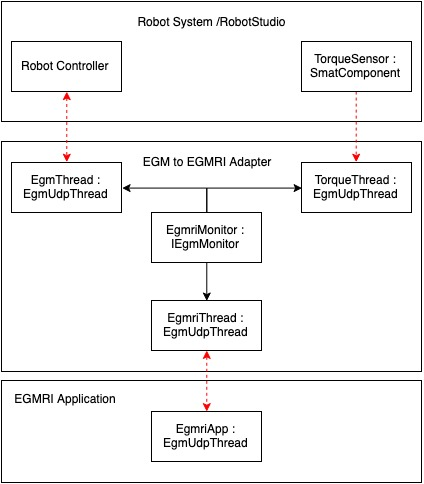
\includegraphics[width=8cm]{egmri.jpg}
    \caption{A hypothetical EGMRI to EGM adapter.}
    \label{fig:egmri_adapter}
\end{figure}
The idea is essentially to implement two endpoints (an application and an adapter). The adapter would communicate with the controller with the EGM protocol via the EgmThread. Torque sensors (the hypothetical implementation of which is discussed in section \ref{app:Hypothetical:torque}) would send relevant joint torque data to the TorqueThread. The logic for creating EGMRI messages from these two sources of data would be in the EgmriMonitor. The EGMRI protocol messages would be sent and received from via the EgmriThread. As it stands, the EgmUdpThread class does not support initiating a UDP connection, but the connection could be initiated in a similar way to the SendState() method in the EgmLineSensor class. Assuming that success of a torque sensor implementation, this model could work.

\newpage
\section{Creating a Virtual Torque Sensor}
\label{app:Hypothetical:torque}
A torque sensor (that could detect the torque of the joint in a simulated robot) could look like figure \ref{fig:torque_sensor}.

\begin{figure}[H]
    \centering
    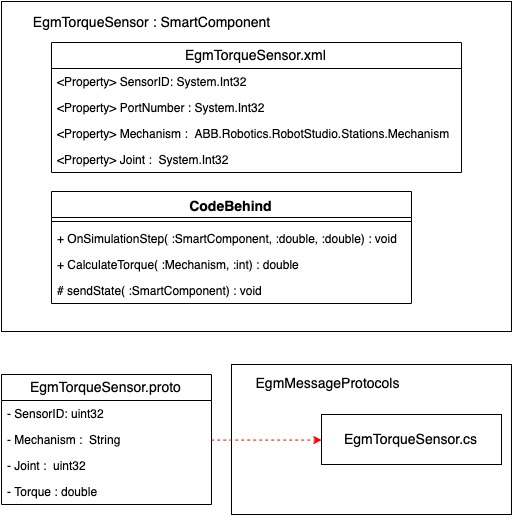
\includegraphics[width=8cm]{torque_sensor.jpg}
    \caption{A hypothetical torque sensor.}
    \label{fig:torque_sensor}
\end{figure}

To calculate torque in a simulation, the smart component will need to extract information from the simulated robot. It would be useful if the choice of the robot and the joint being measured was given to the user, so there could be a property for mechanism and joint defined in the EgmTorqueSensor.xml. The idea is that, once the user asigns this smart component a mechanism and joint, the method CalculateTorque() in the CodeBehind.cs will use those properties to find the appropriate machanism and joint in the simulation, extract the data needed to calculate torque for that joint and then call the SendState() method that will send an EgmTorqueSensor protocol message to the user given port number (xml property). This is a very vague suggestion, but assuming that a smart component can extract the data required to calculate torque, this model should work. The class to serialize and deserialize the protocol messages (EgmTorqueSensor.cs) would not need to be added to the EgmMessagePrototols namespace for this to work. As long as the class is in both the EgmTorqueSensor smart component namespace and the namespace of the IEgmMonitor implementation that receives it, the protocol will work. The advantage of adding EgmTorqueSensor.cs to the smart component and the IEgmMonitor is that the framework would not need to reinstalled in RobotStudio. 

\newpage
\section{EGM and Python}
\label{app:Hypothetical:python}
This project never actually implemented an EGM endpoint in python. However, all of the pieces required for a multi-threaded synchronous UDP communication of google protocol buffer messages via a monitor were implemented \cite{Greg:Jupyter}. That is to say, there is very little difference between the EGM endpoint that was built using the framework for the demonstration (the EgmEndpoint smart component) and the Python code that was developed. The difference is that serialization code for egm.proto was never built. However, other protocol definitions were built into serialization code for Python (i.e. line\_sensor\_pb2.py handles line\_sensor.proto messages). It should be possible to implement an EGM endpoint by:
\begin{enumerate}
    \item Building Python serialization code for egm.proto (egm\_pb2.py)
    \item Making an equivalent of an EgmUdpThread.cs in Python
    \item Making an equivalent on an EgmMonitor in Python
\end{enumerate}
A hypothetical implementation of a Python EgmMonitor and EgmUdpThread can be found in figures \ref{fig:py_monitor} and \ref{fig:py_thread} respectively. 

\lstset{language=Python}
\begin{figure}[H]
\centering
\begin{lstlisting}[fontadjust]
import egm_pb2 as egm_proto

class EgmMonitor():
    
    def __init__(self):
    
    def write(self, portNbr, data):
        egmRobot = egm_proto.EgmRobot()
        egmRobot.ParseFromString(data)
        print egmRobot
            
    def read(self, portNbr):
        egmSensor = egm_proto.EgmSensor()
        # all steps of adding data to EgmSensor message ommited 
        # from example code save space. This is where it would go.
        return egmSensor.SerializeToString()
\end{lstlisting}
\caption{A hypothetical Python implementation of IEgmMonitor.}
\label{fig:py_monitor}
\end{figure}

\lstset{language=Python}
\begin{figure}[H]
\centering
\begin{lstlisting}[fontadjust]
import socket

UDP_IP_ADDRESS = "127.0.0.1"
UDP_PORT_NO = 8080

def egmUdpThread(egmMonitor):
    egmSock = socket.socket(socket.AF_INET, socket.SOCK_DGRAM)
    egmSock.bind((UDP_IP_ADDRESS, UDP_PORT_NO))
    runThread = True
    #print "sensor server started"
    while runThread:
        data, addr = sensorSock.recvfrom(1024)
        if len(data) is not None:
            egmMonitor.write(UDP_PORT_NO, data)
        else:
            print "no sensor data" 
        egmData = egmMonitor.read(UDP_PORT_NO)
        sent = egm.sendto(egmData, addr)
    return
\end{lstlisting}
\caption{A hypothetical Python EgmUdpThread.}
\label{fig:py_thread}
\end{figure}

%*********************************
% END HYPOTHETICAL
%*********************************


%*********************************
% IMPORTANT SCREENSHOTS
%*********************************
\chapter{Useful Screenshots}
\label{app:Screenshots}

\section{Visual Studio: Google Protocol Buffer NuGet Package Details}
\label{app:Screenshots:NuGet}
\begin{figure}[H]
    \centering
    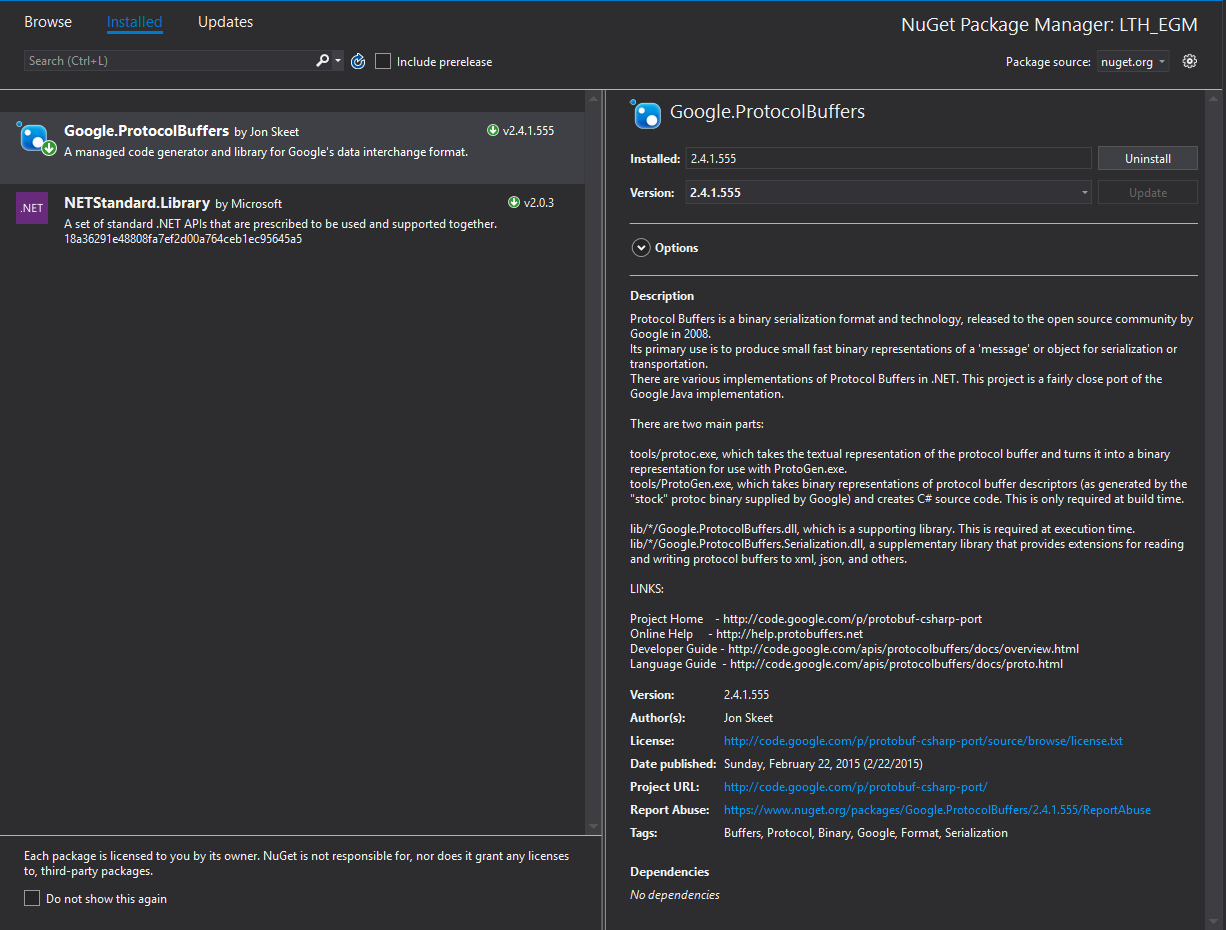
\includegraphics[width=12cm]{gpb_dependency.png}
    \caption{The recommended NuGet package for Google Protocol Buffers.}
    \label{fig:gpb_nuget}
\end{figure}

\section{RobotStudio: EGM RobotWare-option}
\label{app:Screenshots:EGM_in_controller}
\begin{figure}[H]
    \centering
    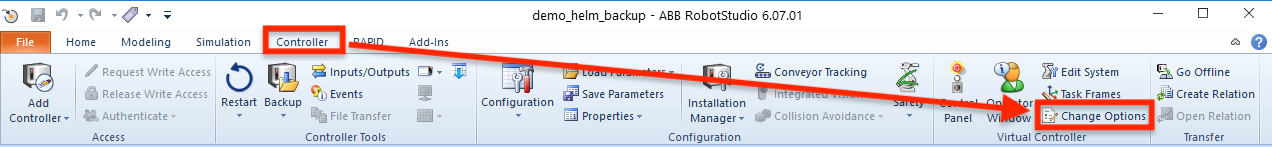
\includegraphics[width=12cm]{egm_controller_settings_mkup1.png}
    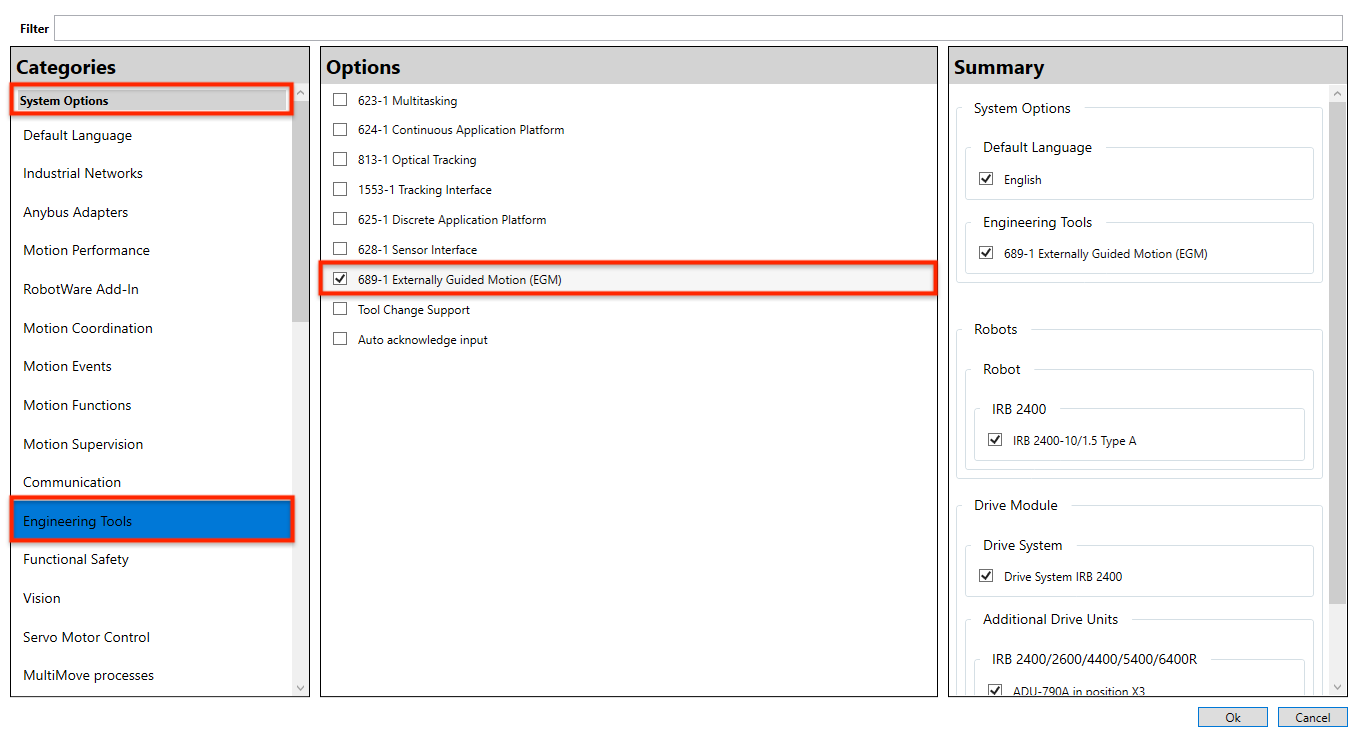
\includegraphics[width=12cm]{egm_controller_settings_mkup2.png}
    \caption{How to enable the EGM RobotWare-option in RobotStudio.}
    \label{fig:egm_option_enable}
\end{figure}

\section{RobotStudio: EGM Transmission Protocols}
\label{app:Screenshots:Trans_protocols}
\begin{figure}[H]
    \centering
    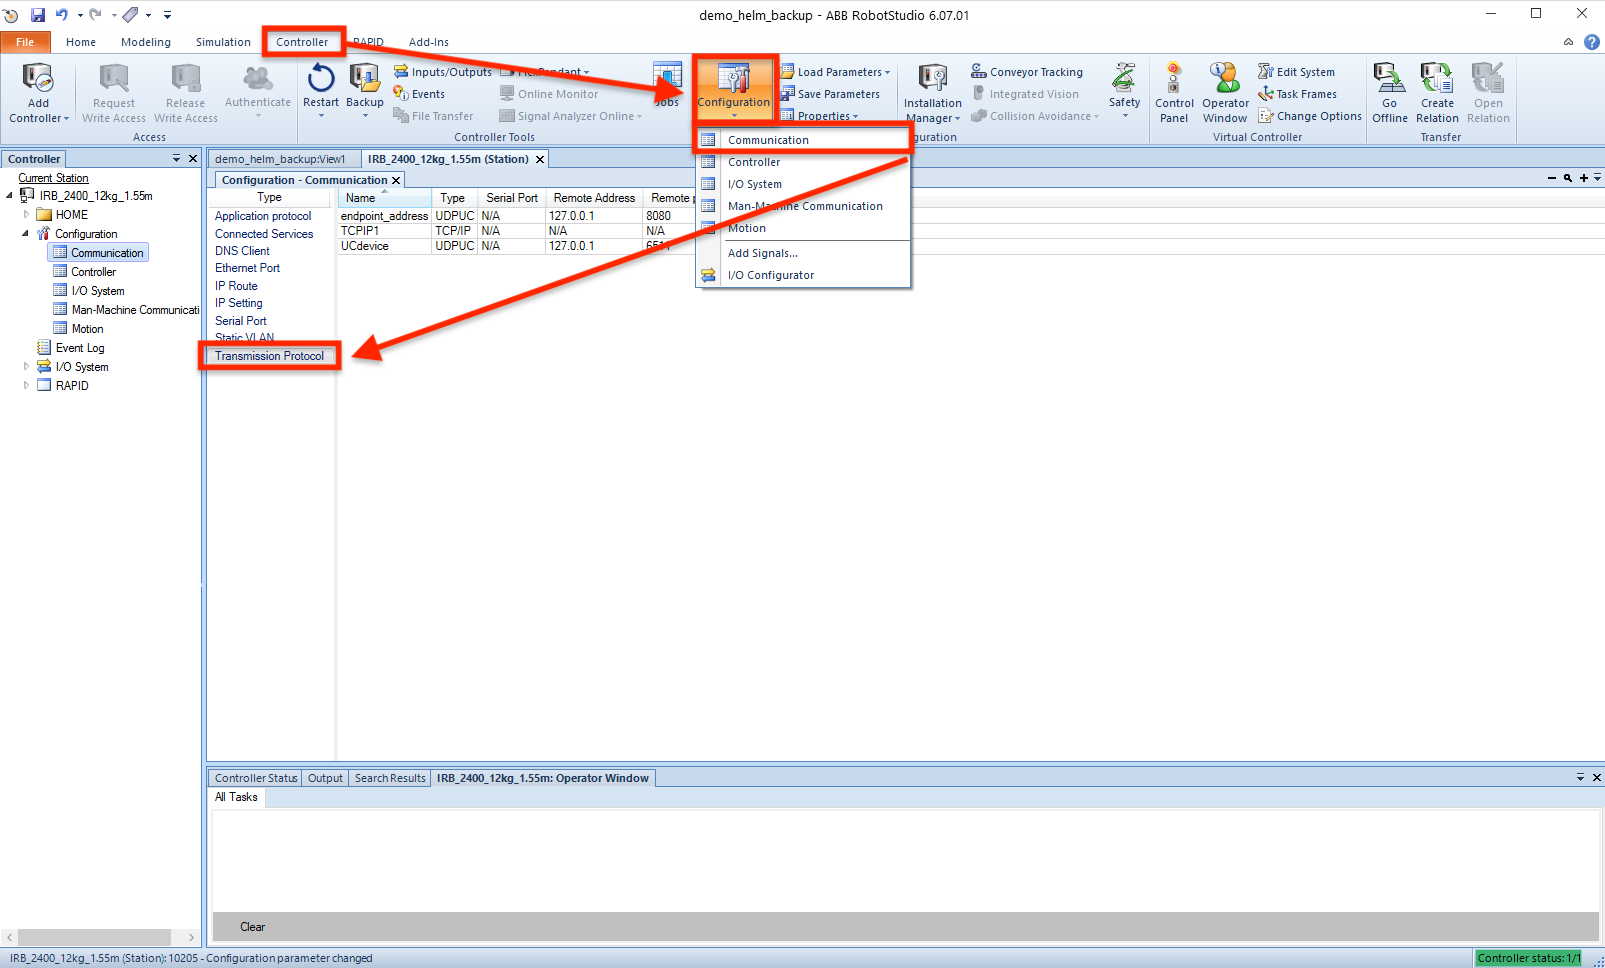
\includegraphics[width=12cm]{egm_trans_proto_lib_markup.png}
    \caption{Where to define a transmission protocol in RobotStudio.}
    \label{fig:egm_trans_proto}
\end{figure}

\section{RobotStudio: EGM Process Parameters}
\label{app:Screenshots:Process_Params}
\begin{figure}[H]
    \centering
    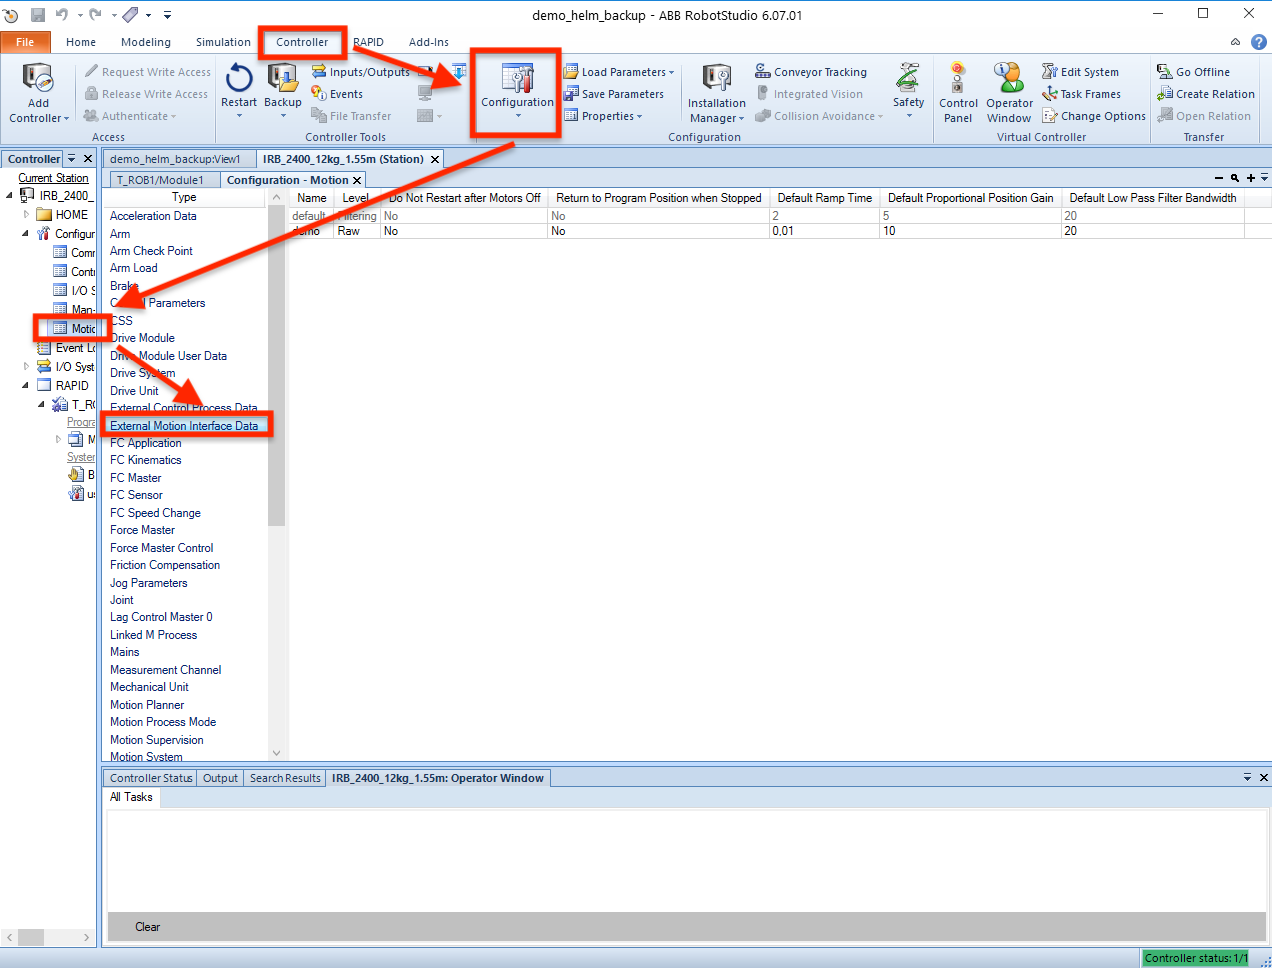
\includegraphics[width=12cm]{egm_connection_markup.png}
    \caption{Where to define the parameters of an EGM Process in RobotStudio.}
    \label{fig:egm_process_parameters}
\end{figure}

%*********************************
% END IMPORTANT SCREENSHOTS
%*********************************


\end{appendices}
\end{document}
